% Measured energy per token (Paper 1). Build: make pdf (tectonic), or pdflatex paper && bibtex paper && pdflatex paper && pdflatex paper.
% Tables in tables/ and figures in figs/ are generated by analysis/build.py from data/features.parquet,
% except figs/fig_experiments (a drawn schematic; source figs/src/fig_experiments.svg).
\documentclass[11pt]{article}
\usepackage[margin=1in]{geometry}
\usepackage[T1]{fontenc}
\usepackage[utf8]{inputenc}
\usepackage{lmodern}
\usepackage{microtype}
\usepackage{graphicx}
\usepackage{booktabs}
\usepackage{longtable}
\usepackage{array}
\usepackage{makecell}
\usepackage{pdflscape}
\usepackage{amsmath}
\usepackage{xcolor}
\usepackage[numbers,sort&compress]{natbib}   % IEEE numeric citations [n]
\usepackage[hidelinks]{hyperref}
\urlstyle{same}
\def\UrlBreaks{\do\/\do\-\do\.\do\_}
\usepackage{caption}
\usepackage[section]{placeins}
\captionsetup{font=small,labelfont=bf}
\setlength{\parskip}{3pt}
\graphicspath{{figs/}}
\hypersetup{pdftitle={Measured Energy per Token for Four Open Language Models on NVIDIA H100 and B200: Batch, Context, Precision, Tensor Parallelism and Prefix Caching},
  pdfauthor={James Manktelow}, pdfkeywords={LLM inference, energy measurement, GPU, H100, B200, vLLM, KV cache, batching}}
% Release identifiers: Zenodo DOI 10.5281/zenodo.24014980 (reserved 6 Nov 2026) in \thanks below and in Section 6.

\title{Measured Energy per Token for Four Open Language Models on NVIDIA H100 and B200,\\Analyzed by Batch, Context, Precision, Tensor Parallelism and Prefix Caching}
\author{James Manktelow\thanks{Version 1.0.1 (November 2026); the repository's changelog lists its corrections to version 1.0.0. Corpus, harness and analysis code: Zenodo, \href{https://doi.org/10.5281/zenodo.24014980}{doi:10.5281/zenodo.24014980}, and \url{https://github.com/InferenceCarbon/measured-energy-per-token}.}\\InferenceCarbon Ltd\\\small ORCID 0009-0003-6822-8300 \quad james.manktelow@inferencecarbon.ai}
\date{}

\begin{document}
\maketitle

\begin{abstract}
How much energy does a GPU use to produce one token of a language model's answer, and what settings move that number? We metered the board energy of rented NVIDIA H100 and B200 GPUs serving four open-weight models (Qwen3-8B, Qwen3-30B-A3B, DeepSeek-V2-Lite and Llama-3.3-70B) with vLLM, in 917 runs over 472 configurations, mainly on two rented pods per GPU type (13 pods in 8 data centers in all). Every figure is gross board energy, idle draw included, over a defined window of requests. Our research shows that batch concurrency was the largest driver of variation: between one request at a time and the highest load we report (60 to 91 requests running on average), energy per output token fell 14- to 42-fold (median 21-fold). Latency increased with batch depth: the median time to first token rose from 0.02 to 0.05 s at one request to 0.2 to 1.0 s at a target of 64. Reusing a cached prompt came next: a request whose first 16k tokens were already in the server's cache used 1.5 to 6 times less energy than an uncached request of the same length. Running past the server's memory for stored context raised energy per token 4- to 6-fold, and a longer context raised it 1.3 to 2.7 times at a target batch of 8. Splitting a model over additional GPUs cost 7 to 40\% more energy per token for 1.1 to 1.6 times the throughput, and 4-bit (nvfp4) versions of two of the models, as published by Red Hat and NVIDIA, used 14 to 39\% less energy per output token than the 8-bit versions on B200 (one pod per model). At the same target batch and on the same number of GPUs, the B200 gave no consistent saving over the H100 (a median 0.93 of its energy per token, from 0.75 to 2.7 depending on the model), a comparison that leaves the faster GPU less fully used: at one request at a time neither GPU reached two-thirds of its memory-bandwidth bound, and the B200 was further from it than the H100 for every model. Serving Llama-3.3-70B on one B200 instead of the two H100s it needed used 7 to 30\% less energy per token at batches 1 to 64, partly from using fewer GPUs. A loaded, idle GPU drew about a fifth (H100) to a quarter (B200) of its rated power. The corpus, harness and analysis script are released with the paper.
\end{abstract}

\section{Introduction}\label{sec:intro}

Published figures for the energy of one token of language-model inference span two orders of magnitude, from a few hundredths of a joule per output token for models in their lowest-energy configurations on B200 GPUs~\citep{chung2026joules} to 3 to 4~J for a 65-billion-parameter model on older GPUs~\citep{samsi2023words}. Part of that spread reflects what each study held fixed: the size of the batch the server ran, the context it attended to, the precision of its weights, how many GPUs shared the model, and whether the prompt was already in the server's cache. Few published measurements vary these together on the same hardware with the same serving software, and fewer still say how much the result moves from one rented pod to the next. That matters to anyone who must report or reduce the energy of AI use: without knowing which settings move the figure, a published number can neither be checked nor carried over to another deployment.

This paper reports such a set of measurements, and its key finding is that batch depth dominates. On a single GPU (two for Llama-3.3-70B on H100), energy per output token at one request at a time was 14 to 42 times the energy at the highest load we report, for every model and both GPU generations (Section~\ref{sec:batch}). Context, precision, tensor parallelism and the choice of GPU each moved it by a factor of 4.7 or less over the ranges we tested, except where a long context also forced a smaller batch (up to 9.8 times). On the same number of GPUs, at the tested settings, the newer B200 gave no consistent per-token energy saving over the H100 (Section~\ref{sec:b200}). A cached prefix cut whole-request energy by up to six times. A server pushed past the capacity of its memory for stored context (the KV cache) stalled rather than slowed (Section~\ref{sec:kv}): throughput fell 3.4- to 5.3-fold while board power rose 10 to 22\%, so energy per token rose 4.1- to 5.8-fold. Section~\ref{sec:factors} compares the factors.

The paper makes four contributions. First, it measures how far each serving setting moves energy per token on one serving stack under one metering protocol, so that the settings can be compared on a single scale (Section~\ref{sec:factors}). Earlier measurements report energy for chosen workloads or for each GPU's best configuration, and model-based estimates assume the settings. Second, it measures two effects of request shape directly: the saving from reusing a cached prefix, against an uncached control of the same length, and the cost of running past the capacity of the KV cache, located by shrinking the memory the server was given. Third, it reports how far each figure moved between rented pods, for the 413 configurations run on two pods, and it reports the loaded-idle draw separately from the energy of each window. Fourth, it publishes the corpus, with every window's raw power samples, and the script that produces every number in the paper, so that estimation methods can be calibrated and checked against measured data.

We wrote this for three readers: engineers who serve open models and want to know which settings move energy per token, analysts and regulators who need measured figures with stated boundaries to check published claims against, and the authors of estimation methods, who need a measured corpus to calibrate on.

Six terms recur. A \emph{token} is the unit a model reads and writes, about three-quarters of a word of English. A request has two phases: \emph{prefill}, in which the server reads the prompt, and \emph{decode}, in which it writes the answer one token at a time. The \emph{batch} is the number of requests the server advances together in one decode step, so that one read of the model's weights serves all of them (for a mixture-of-experts model, one read of each expert the batch uses). The \emph{KV cache} (keys and values) holds, for every token in every running request, the intermediate values that later tokens attend to. The cache grows with the context and bounds the batch a GPU can hold. A \emph{cached prefix} is a leading part of a prompt the server has already processed and can reuse. We measured \emph{workloads} built so that most of the work is one phase, not phases in isolation (Section~\ref{sec:experiments}). Appendix~\ref{app:glossary} defines the rest of the vocabulary.

We served four open-weight models with vLLM~\citep{kwon2023vllm,vllm0151} on rented single-node pods carrying NVIDIA H100 (80 GB memory) and B200 (180 GB memory) GPUs, and read the GPUs' own energy counters. The corpus holds 917 runs over 472 configurations, of which 438 have two usable repeats and 413 were run on two pods. The figures are gross board energy: whatever the GPU boards drew during a measurement, idle draw included, divided by the output tokens (for the prefill workload, the prompt tokens) of the requests in it. Section~\ref{sec:boundary} gives the boundary.

This paper is a measurement report. It fits no energy model, makes no estimate for models or hardware we did not run, and converts nothing to carbon.

\section{Related work}

Direct measurement of open models is well established. \citet{samsi2023words} metered LLaMA models of up to 65 billion parameters on V100 and A100 GPUs, sharded over up to 32 GPUs, and measured about 3 to 4 J per output token for the largest model, rising as the model was spread over more GPUs.

The ML.ENERGY benchmark~\citep{chung2025mlenergy} metered energy per whole response for 40 model architectures across six tasks on A100 and H100 GPUs, each task with a fixed request dataset. It found that the server's maximum batch size dominated: for reasoning models on H100, energy per response fell by up to about sixfold between a maximum batch of 4 and one of 64. It also found that GPUs serving a language model drew much less power than their maximum, because decoding does little computation for each byte it reads from memory. Its follow-up~\citep{chung2026joules} reported 1,858 configurations of 46 models, diffusion models as well as language models, across seven tasks on H100 and B200 GPUs. Reasoning tasks there used on average about 25 times the energy per response of chat, from ten times the output tokens and a higher energy per token, because longer outputs left less memory for batching. It compared the two GPUs by choosing each one's minimum-energy configuration at each of three latency limits, and found the B200 lower in 63 of 72 language-model comparisons, by a median 35\%. At the tightest limit, more H100s sometimes used less energy than fewer B200s.

Power measurements beyond the board point the same way. \citet{patel2024power} found, on servers like those of a large cloud provider, that prompt processing briefly reached or exceeded the GPUs' rated power while token generation, which lasts longer, drew less. Across production inference clusters this left about 21\% headroom between peak and provisioned power, against about 3\% for training clusters. \citet{latif2025singlenode} measured an 8-GPU H100 node during training and recorded a peak of about 8.4 kW, 18\% below its 10.2 kW rating. Using those measurements, \citet{newkirk2025calibrated} found that even computationally intensive training drew on average no more than 76\% of the rating, and built a node power model with an 11.4\% mean error, against 27 to 37\% for estimates based on rated power.

Model-based estimates fill in serving conditions by assumption. \citet{jegham2025hungry} estimated 30 models served in commercial data centers from public API performance data, inferred hardware and provider-specific multipliers, and put the most energy-intensive above 29 Wh for a long prompt. \citet{oviedo2026energy} built a bottom-up estimate under production assumptions, put the median query to a frontier-scale model (more than 200 billion parameters) on H100 at 0.31 Wh, and concluded that widely cited estimates were four to twenty times too high. Both depend on the batch, context and caching that a server actually runs, which are the settings we measure. We add controlled measurements of request shape on one stack, varied one or two settings at a time, with the spread between rented pods, the loaded-idle draw and the raw records published.

\section{Method}

To define our method, we describe the pods, the serving stack, the meter, its boundary, the experiments and the statistics, in that order. Serving settings and the meter's internals are in Appendix~\ref{app:detail}.

\subsection{Pods, dates and versions}\label{sec:method_pods}

All measurements were made between 22 and 26 October 2026 on 13 rented pods from one cloud GPU marketplace, in 8 data centers in North America, Europe and India (Table~\ref{tab:pods}), with vLLM 0.15.1 in the container \path{runpod/pytorch:1.4.1-cu1281-torch280-ubuntu2404}. The PyTorch and CUDA versions installed with vLLM were not recorded. The NVIDIA driver, 595.91.07, is recorded for four pods, two of each accelerator. H100 pods carried two H100 SXM GPUs (80 GB memory) (one carried four, for tensor parallelism), and B200 pods one B200 SXM GPU (180 GB memory) (two carried two or four). Clock locking was not permitted, so every run used the default power management. The power limit was 700 W on every H100 window and 1,000 W on every B200 window, equal to each board's rated maximum.

The harness changed 13 times during the five days of measurement, and each run records the version it ran under (the deposited code lists the versions and their differences). The meter and the load generator were identical in every version. The changes were to the campaign's orchestration and telemetry, to the prompt-sizing margin at the native-maximum context (Appendix~\ref{app:cells}) and to the memory offered to the nvfp4 servers (Appendix~\ref{app:detail}).

\subsection{Models and serving}

The four models (Table~\ref{tab:models}) span dense and mixture-of-experts (MoE) designs and 8 to 71 billion parameters. All were served by vLLM with fp8 (8-bit floating point) weights and KV cache, prefix caching on except in the cache-miss experiment, a server limit of 256 requests in flight and speculative decoding off. The load generator opened at most 100 connections (its HTTP library's default), which capped the requests running at once (Section~\ref{sec:batch}). With these settings Llama-3.3-70B could not be served on one H100 and ran on two with tensor parallelism (each layer split across GPUs that compute together). It fitted on one B200. The nvfp4 experiment (4-bit floating point with block scaling, a Blackwell-only format) ran on B200 with 4-bit versions of Qwen3-8B and Llama-3.3-70B that Red Hat and NVIDIA had already converted and published. We did not convert any model to 4-bit ourselves. Appendix~\ref{app:detail} gives the remaining settings.

\begin{table}[t]
\centering\small
\caption{The four models. Parameters are in billions. For a mixture-of-experts (MoE) model only part of the weights serves each token (``active''). Context is the model's window in tokens. Three models ran from 8-bit (fp8) versions published by their developers or by Red Hat. For DeepSeek-V2-Lite, vLLM converted the original 16-bit (bf16) weights to fp8 as it loaded them.}\label{tab:models}
\footnotesize
\begin{tabular}{lllrrl}
\toprule
Model & Type & Attention & Total B & Active B & Context \\
\midrule
Qwen3-8B & dense & standard (grouped-query) & 8.2 & 8.2 & 32,768 \\
Qwen3-30B-A3B & MoE, 128 experts, 8 used & standard (grouped-query) & 30.5 & 3.3 & 32,768 \\
DeepSeek-V2-Lite & MoE, 64 experts, 6 used + 2 shared & multi-head latent & 15.7 & 2.4 & 32,768 \\
Llama-3.3-70B & dense & standard (grouped-query) & 70.6 & 70.6 & 131,072 \\
\bottomrule
\end{tabular}
\end{table}

\subsection{Power metering}\label{sec:power}

The energy of a window was read from each GPU board's own running energy total: the total at the end of the window minus the total at the start, summed over the participating GPUs. Before measuring on a pod the harness checked the meter through NVML (NVIDIA's management library~\citep{nvml}) and recorded the driver, the power limit and the clocks. Both the energy total and the power reading changed about every 0.1 s, but that is their update rate, not their averaging interval: NVIDIA documents the power reading on these GPUs as a one-second average, and we did not establish the counter's response time or absolute accuracy. Power samples taken ten times a second and stored raw agreed with the counter to a median absolute difference of 0.08\% (Appendix~\ref{app:detail}), a consistency check rather than a calibration, since both may share the board's telemetry. Energy per output token divides a window's energy by the output tokens of its requests, energy per prompt token (prefill workload) by their prompt tokens, per-request energy by the requests completed, and per-step energy of a simulated agent by its steps. The idle draw and all concurrent work, including the prefill of each request's fresh input, are inside the numerator. These are alternative divisions of the same gross window energy, not components of it. They should not be added: a request's energy is not its prompt tokens times the prefill figure plus its output tokens times the decode figure, which would count the idle draw and the fresh input twice. Dividing a window's energy among its idle draw, its prompt tokens and its output tokens would require a model fitted across experiments.

For every window, the corpus records the duration, the idle power before and after the window, the prompt and output token counts, and the server's prefix-cache counters. A fit could start from these, and we leave it to future work. The corpus does not record directly how many prompt tokens each request read from the cache, and under memory pressure the server's counters count repeated cache lookups, not tokens processed.

\subsection{What is and is not metered}\label{sec:boundary}

The figures are \emph{gross board energy}: the energy the GPU boards drew during the metered window, with nothing subtracted. The boundary was the GPU board. Outside it lie the host CPU and memory, the network, the load-generating client, chassis fans and power-supply losses, the data center overhead usually expressed as PUE (power usage effectiveness, facility energy over IT energy), the embodied energy of the hardware, and the energy of training the model. We did not meter them and we report nothing for them. Because they are outside the boundary, every figure here is a lower bound on the energy a data center spent on the same tokens, and the size of the gap is not measured. Inside the boundary lies the board's idle draw with the model loaded, 17 to 25\% of rated power (Section~\ref{sec:idle}). We report that draw separately but do not subtract it, because it is a real cost of the window and because subtracting it depends on a choice of baseline. A reader who wants an idle-subtracted figure can form one. Each run measured 60 seconds of idle power before and after its window. Where the two differed by more than 5\%, the run was kept and given an idle-drift flag.

\subsection{Experiments, configurations and runs}\label{sec:experiments}

We organized the measurements as ten \emph{experiments}, each answering one question, such as how energy per token changes with the batch. An experiment varied one or two settings (in the batch experiment, the number of requests running simultaneously) and held the others fixed (the prompt length, the answer length and the weight precision). Within an experiment, a \emph{configuration} was one combination of settings for one model on one accelerator: for example, Qwen3-8B on one H100 at a target batch of 16. A \emph{run} was one metered execution of a configuration. Most configurations were run twice (Section~\ref{sec:stats}). Appendix~\ref{app:cells} lists the ten experiments and their settings. Figure~\ref{fig:experiments} summarizes the experiments, how a run proceeded and the shape of a decode request. We refer to them by the short labels c0 to c9b that the deposited data use: c1 is the batch experiment, c2 the context experiment, and so on.

A run proceeded as a 60 s idle window, cache warming and up to four warm-up requests, the metered window, and a second 60 s idle window. The meter started after warm-up with no request in flight. During the window a fixed number of client workers each kept one request in flight: the \emph{target batch}, or desired concurrency. Requests were issued until the window reached 60 s and 20,000 tokens, then drained before the meter stopped, so every request's energy and tokens fall inside the same window. The idle experiment (c0) and the simulated agent (c8) follow their own rules (Appendix~\ref{app:cells}). The \emph{achieved batch} we plot is the server's mean count of running requests, read every 0.5 s over the middle 80\% of the window. Where the harness predicted that the KV cache could not hold the target, it ran a smaller one and recorded it. The two runs of a configuration went to different pods where we had access to two of the accelerator type.

Every experiment used synthetic prompts with the shape of one step of an agentic request, in which a program rather than a person calls the model repeatedly. Each prompt had a long block that stays the same from call to call and can be cached (an opening instruction and a record of the work so far), then a short block that is new on every call (standing for what a tool returned), then a one-line instruction. A decode-workload request therefore carried a cached 1k-token prefix, about 200 fresh input tokens that the server read inside the window, and asked for 256 output tokens. There were as many distinct cached prefixes as the target batch (256 at a target of 256), each warmed before the window, and each request reused one of them. Raising the target therefore also raised the number of prefixes the server had to keep. Requests were streamed at temperature 0 with a fixed seed, and token counts came from the server's own usage report. The simulated-agent experiment (c8) chains such steps into a growing context (Section~\ref{sec:agent}). Appendix~\ref{app:detail} gives the construction.

\begin{figure}[t]
\centering
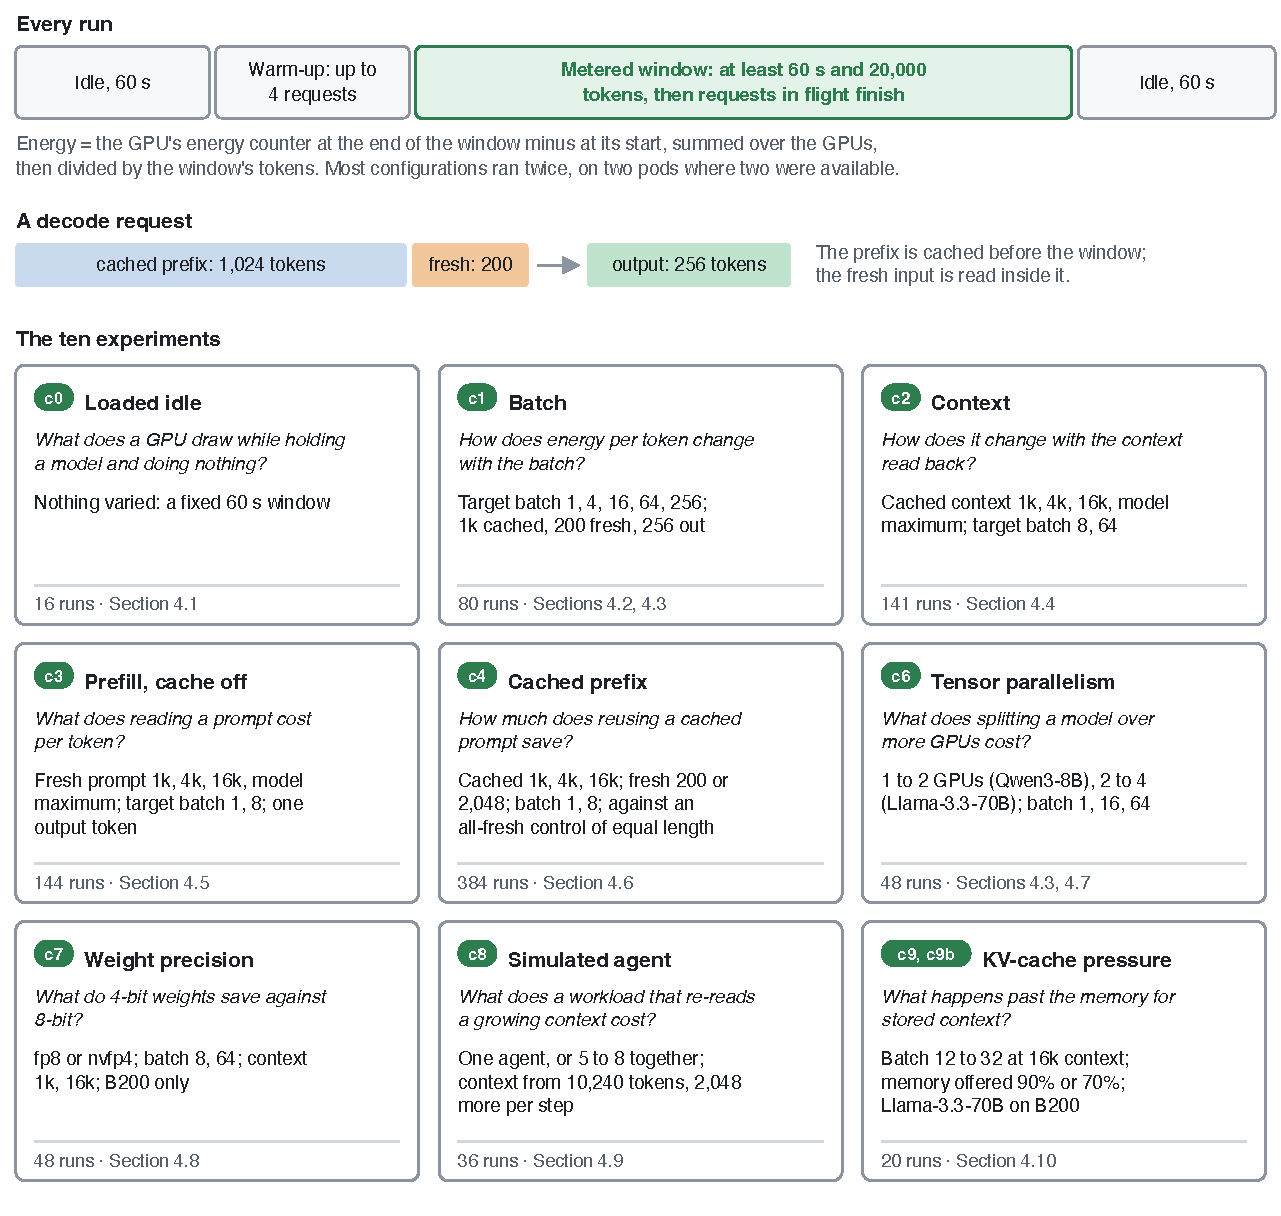
\includegraphics[width=\textwidth]{fig_experiments}
\caption{The experiments. Top: the steps of every run. Middle: the shape of a decode-workload request. Bottom: the ten experiments, each with the question it answers, the settings it varied, its number of runs and the section that reports it. Experiments c9 and c9b share a card. Table~\ref{tab:cells} (Appendix~\ref{app:cells}) gives every setting.}\label{fig:experiments}
\end{figure}

\subsection{Corpus and statistics}\label{sec:stats}

The corpus comprises one row per run: 917 runs, of which 902 enter the analysis.

Of the 15 runs that do not enter the analysis, four have no usable active window: Qwen3-8B decode runs at a 32,768-token cached context, all refused by the server's context limit of 32,512 tokens. Eleven more are excluded because the server's prefix-cache counters show that their cached context was recomputed on most requests during the window, so they are not the shape their configuration states (Appendix~\ref{app:tables} lists them and the rule, added in version 1.0.1).

Table~\ref{tab:corpus} gives runs per experiment, model and accelerator, Table~\ref{tab:pods} the pods, and Appendix~\ref{app:tables} the full tables. Of the 472 configurations, 438 have two usable runs, 26 one and 8 none; 413 were run on two pods and 59 on one. Five configurations with two runs enter no variability table because one run lacks a prompt-token count (Llama-3.3-70B prefill on H100), so 433 configurations appear there. The analysis script (\path{analysis/build.py}) produces every table and figure from the corpus file.

For every reported quantity we give a central value, a band and the number of pods behind it. The central value is the mean over the configuration's runs. No configuration ran on more than two pods, and most ran once on each of two, so the band is the range of the two runs: between pods where there were two, between repeats on one pod otherwise. For a ratio whose two sides ran on different pods, the band runs from the lowest combination of the two sides' runs to the highest. A range of two values is the observed spread between the pods we rented, not a confidence interval (a conventional 90\% interval for the mean of two values would be about six times wider) and not an accuracy figure for the meter. It captures what differs between pods (host, firmware, neighbors) and nothing held fixed across them: the serving stack and its settings, the prompt shape, any bias the counter shares across boards, or the marketplace's hardware population. Repeats on one pod agreed more closely (the two runs differed by a median 0.6\% of their mean, 30 configurations) than repeats on two pods (2.7\%, 124), which suggests that the pod sets most of a band's width, although the two sets hold different configurations. A third pod would characterize the spread between deployments better, and could widen the bands.

We attach no confidence labels. Each table states what a figure rests on: the Pods column gives the number of pods, and a single run is marked n=1. A ratio compares two sets of runs, its two \emph{sides}. Where both sides ran on the same pods we report the mean of the per-pod ratios, so that a pod's own conditions (power limit, clock policy) affect both sides alike, and where they ran on one pod we pair by repeat. Otherwise (every B200 to H100 ratio, and some tensor-parallel and precision ratios) the ratio is of the two central values and the band carries the spread of both. In the text, ``$x$ [$a$, $b$]'' means central value $x$ with band $a$ to $b$, and a figure quoted without a band is a ratio of central values.

\section{Results}

This section reports what each factor did to energy per token, one factor per subsection. It starts with the power a GPU drew while holding a model and doing nothing, because that floor sits under every other figure, and it ends (Section~\ref{sec:factors}) by comparing all the factors on one scale. Full tables are in Appendix~\ref{app:tables}.

\subsection{Loaded-idle power}\label{sec:idle}

With a model loaded into GPU memory and no requests to serve, an H100 drew 123 to 130 W (18 to 19\% of its 700 W rating) and a B200 244 to 245 W (24\% of 1,000 W), as means per GPU over the four models (Table~\ref{tab:idle}). The two-GPU Llama-3.3-70B server drew 259 [249, 270] W in all.

At one request at a time a B200 drew only 368 to 679 W, so its 245 W idle floor was 57\% of that draw (median over the runs of the four models, range 35 to 68\%). On H100 it was 39\% (27 to 51\%). At the highest load the shares fell to 35\% and 23\% (Table~\ref{tab:idle_share}).

This is a reference ratio, not a component isolated inside the window. A reader who subtracts idle power from our batch-1 figures will roughly halve them, and one who subtracts it from the highest-load figures will cut them by a quarter to a third. Decode windows ran at 35 to 93\% of rated board power across the batch grid, consistent with the below-rated serving power reported by \citet{patel2024power}.

\subsection{Energy per output token against batch}\label{sec:batch}

Energy per output token of the decode workload fell 14- to 42-fold between one request at a time and the highest load we report, on a single GPU or the H100 pair (Figure~\ref{fig:batch}, Table~\ref{tab:decode_batch}). That load was 256 requests in flight for seven of the eight model and GPU pairs, of which the server ran 67 to 91 on average: the client's 100-connection limit capped the running requests, and the KV cache was only 1 to 23\% full. For Llama-3.3-70B on two H100s it was the target of 64 (achieved 60), since its target-256 runs are excluded (below). The deepest point is therefore the highest load we offered or report, not the most a GPU could hold. For each model, from one request at a time to the highest load, with the fall as a ratio of central values:
\begin{itemize}
\item Qwen3-8B: 2.61 [2.60, 2.62] to 0.085 [0.0849, 0.0851] J per token on H100 (31-fold, achieved batch 84), and 2.10 [2.00, 2.20] to 0.0912 [0.0910, 0.0914] on B200 (23-fold, batch 67);
\item Qwen3-30B-A3B: 1.67 [1.66, 1.67] to 0.1226 [0.1225, 0.1226] on H100 (14-fold, batch 90), and 1.41 [1.34, 1.47] to 0.092 [0.092, 0.093] on B200 (15-fold, batch 79);
\item DeepSeek-V2-Lite: 1.05 [1.04, 1.06] to 0.066 [0.064, 0.068] on H100 (16-fold, batch 84), and 1.48 [1.44, 1.52] to 0.080 [0.080, 0.081] on B200 (18-fold, batch 77);
\item Llama-3.3-70B: 15.4 [15.1, 15.7] to 0.541 [0.532, 0.550] on two H100s (28-fold, batch 60, target 64), and 14.3 [13.4, 15.2] to 0.34 [0.33, 0.34] on one B200 (42-fold, batch 91).
\end{itemize}
The H100 figures at a target of 256 rest on one pod, which ran both repeats.

Most of the saving came at the lower batches and slowed at the highest loads. On H100, DeepSeek-V2-Lite even cost more at the highest load than at a target of 64.

At one request at a time, the dense Qwen3-8B cost 1.6 to 2.5 times as much per token as the two MoE models on H100, and 1.4 to 1.5 times on B200. The likely cause is the weights. At batch 1 every token pays for a full read of the weights it uses, and the dense model uses more of them: 8.2 billion active parameters against 2.4 to 3.3 billion. Batching shares that read across requests, so the gap closed, and at the highest load the three smaller models cost 0.066 to 0.123 J per token. The MoE models share less, because different requests can use different experts, so each step reads more weights as the batch grows.

At one request at a time, neither GPU came close to its speed limit. Each decode step reads the model's weights once, so the token rate cannot exceed the memory bandwidth divided by the bytes read (Table~\ref{tab:roofline}; bandwidths from NVIDIA~\citep{nvidia_specs}). The measured rate was 8 to 64\% of that limit, and the idle draw was 27 to 67\% of board power. At batch 1, most of a token's energy therefore pays for the server's fixed cost per step and the idle floor. Batching saves energy mainly by spreading those costs over more tokens: on average, each doubling of the batch cut energy per token by a factor of 1.49 to 1.78 (median 1.63).

Batching also costs latency (Table~\ref{tab:latency}). The median time to first token rose from 0.02 to 0.05 s at one request to 0.2 to 1.0 s at a target of 64, and to 6 to 12 s at 256, where requests waited for a connection. The interval between output tokens rose from 4 to 21 ms to 9 to 33 ms.

One model did not follow the pattern: on H100, DeepSeek-V2-Lite cost 1.4 times as much per token at the highest load as at a target of 64, which we cannot explain, since its cache was 3\% full and its hit rate normal. Llama-3.3-70B on two H100s had cost 1.3 times as much at a target of 256 as at 64 in version 1.0.0 of this paper, and its server's counters showed a prefix-cache hit rate of only 0.36 to 0.39 against 0.84 in every other run. The check added in version 1.0.1 (Appendix~\ref{app:tables}) confirms the cause: with 256 cached prefixes beside the running requests, the server's memory could not hold them all, so it discarded prefixes and recomputed them on more than half the requests. Those two runs are not the cached-prefix shape the configuration states and are excluded; Llama-3.3-70B's highest reported load on H100 is therefore the target of 64.

At the highest reported load, Llama-3.3-70B produced 2,300 [2,282, 2,318] tokens per second on two H100s (target 64) and 2,744 [2,689, 2,799] on one B200 (target 256), and the three smaller models 4,430 to 7,800.

\begin{figure}[t]
\centering
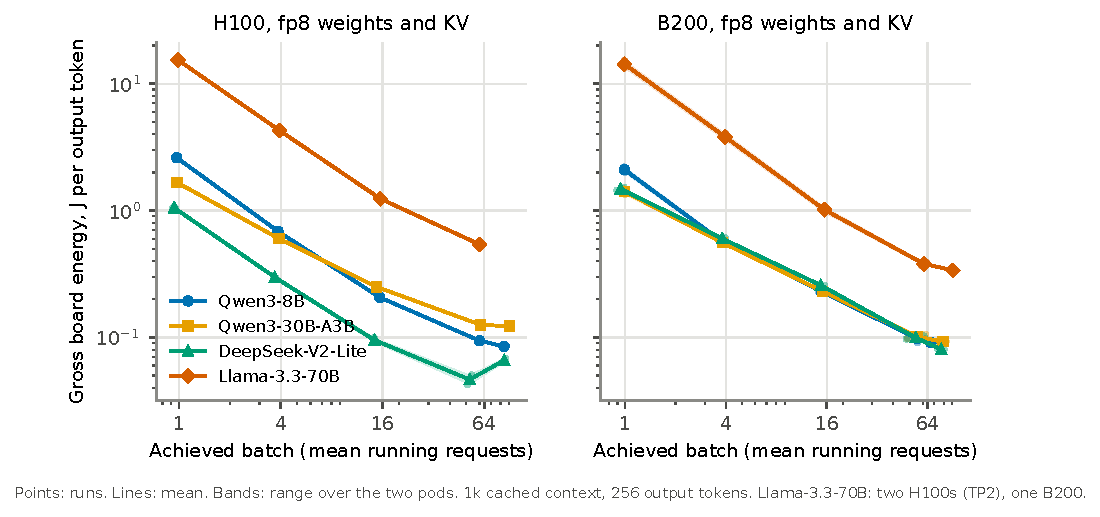
\includegraphics[width=\textwidth]{fig1_decode_batch}
\caption{Energy per output token of the decode workload (gross board energy including the idle draw) against achieved batch, the server's mean count of running requests, experiment c1. Points are runs, lines the mean per target batch, bands the range over the two pods. 1k cached context, 200 fresh input tokens, 256 output tokens, fp8 weights and KV cache. The rightmost points are a target of 256 (Section~\ref{sec:batch}). Llama-3.3-70B runs on two H100s (TP2) and one B200.}\label{fig:batch}
\end{figure}

\subsection{B200 against H100}\label{sec:b200}

On the same number of GPUs, the B200 gave no consistent saving over the H100 (Figure~\ref{fig:b200}, left, and Table~\ref{tab:b200_h100}). Across 24 comparisons it used a median 0.93 of the H100's energy per token, and the direction depended on the model:
\begin{itemize}
\item Qwen3-30B-A3B used less on B200 at every batch (0.75 to 0.93).
\item Qwen3-8B used less at batches 1 and 4 (0.80 [0.76, 0.85] and 0.83 [0.79, 0.86]) and on two GPUs each (0.82 to 0.91), but 1.04 to 1.11 times as much on one GPU at batch 16 and above.
\item DeepSeek-V2-Lite used \emph{more} on B200 at every batch: 1.41 [1.36, 1.46] at batch 1, up to 2.70 [2.60, 2.82] at batch 16, and 1.22 [1.17, 1.27] at the highest load. At similar throughput its B200 drew 368 to 654 W against 265 to 411 W on H100. It has the smallest active parameter count of the four (2.4 billion) and multi-head latent attention, either of which may matter. We did not test them.
\item Llama-3.3-70B, on two and on four GPUs each, went from 1.03 [0.99, 1.07] and 1.10 at batch 1 to 0.80 [0.78, 0.81] and 0.90 at batch 64 (the B200 side on one pod).
\end{itemize}
The same target batch leaves the faster GPU less fully used: at one request the B200 reached a smaller share of its bandwidth bound than the H100 for every model (Table~\ref{tab:roofline}), and it idles at about twice the power. A comparison at matched throughput or matched latency, which Table~\ref{tab:decode_batch} allows, is the one an operator would make. How well this version of vLLM's kernels used Blackwell may also contribute; we did not profile it. These ratios compare the two GPUs at the same GPU count, offered load and serving settings. They do not compare each GPU at its best, as \citet{chung2026joules} do under a latency limit, and the same target batch does not guarantee the same achieved batch or latency.

The B200's larger memory matters most for the largest model (Figure~\ref{fig:b200}, right). At fp8, Llama-3.3-70B's weights take about 70 GB of an H100's 80 GB of memory, leaving little room for stored context (about 160 KiB per token), so with our settings it needed two H100s but fitted on one B200.

One B200 used 0.93 [0.85, 1.00] of the energy per token of two H100s at batch 1 and 0.70 [0.67, 0.74] at batch 64. This ratio is the product of two we measured, so the saving can be split. Using one GPU instead of two saved about 12\% at every batch (Table~\ref{tab:tp}). The newer GPU saved nothing at batch 1 (two B200s used 1.03 of two H100s) but 20\% at batch 64 (0.80). Its advantage probably grows with load because a B200 idles at about twice the power of an H100 (Table~\ref{tab:idle}), a floor that more tokens share at higher load. At a target of 256 the two H100s recomputed most of their cached prefixes (Section~\ref{sec:batch}), so the comparison stops at batch 64; version 1.0.0 reported 0.48 at that point.

\begin{figure}[t]
\centering
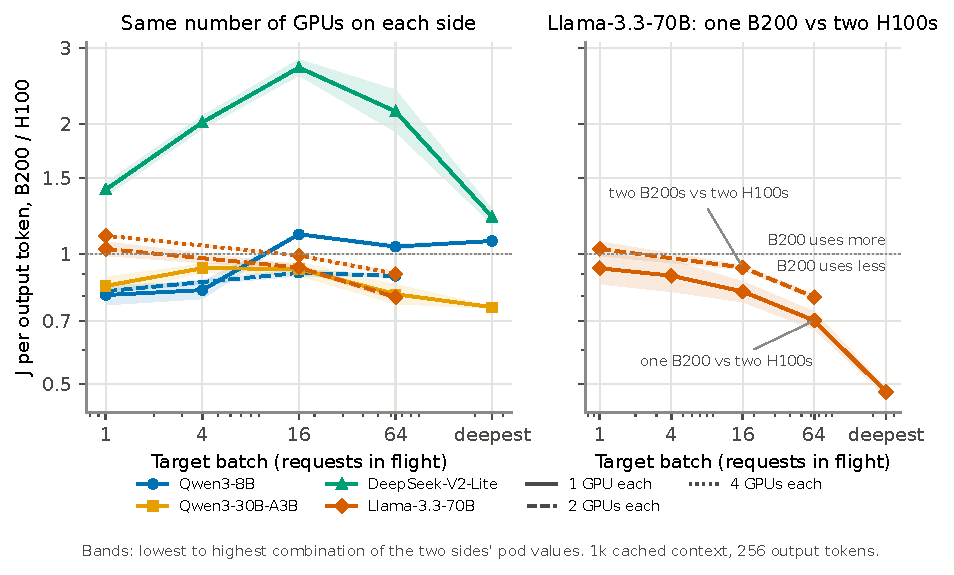
\includegraphics[width=0.92\textwidth]{fig_b200_h100}
\caption{B200 over H100: energy per output token of the decode workload at the same target batch (1k cached context, 256 output tokens). Below 1, the B200 used less. Left: the same number of GPUs on each side, one each (solid, experiment c1), two each (dashed, c6) and four each (dotted, c6). Right: Llama-3.3-70B on one B200 against the two H100s it needed (solid), and two B200s against two H100s (dashed). The gap between the lines is the saving from serving on one GPU. Bands: lowest to highest combination of the two sides' pod values. At the highest target (256), 67 to 91 requests ran at a time on average.}\label{fig:b200}
\end{figure}

\subsection{Energy per output token against context}\label{sec:context}

Energy per output token rose with context in every configuration, and rose more at the deeper batch (Figure~\ref{fig:context}, Table~\ref{tab:decode_context}). Here context means everything the model reads back while writing: the cached prefix, the fresh input and, on average, half the answer so far. At a design batch of 8, going from 1k tokens to the 31k to 32k maximum of the three smaller models raised energy per token 1.4 to 2.7 times (ratios of central values). DeepSeek-V2-Lite, whose latent attention stores a compressed cache, rose least (1.40 on H100, 1.50 on B200) and Qwen3-8B most (2.69 and 2.31). Llama-3.3-70B rose 1.26 to 1.31 times from 1k to 16k. At its 125k maximum, where the batch had to be cut to 4, it cost 8.42 [7.84, 8.99] J per token on B200 against 1.91 [1.81, 2.02] at 1k. On two H100s, with the batch cut to 3, the one run that kept its cache cost 11.4 J per token; its repeat recomputed the context on every request and is excluded (Appendix~\ref{app:tables}; version 1.0.0 printed both, 11.4 and 44.1, as a collapsed pair).

At a design batch of 64, the memory for stored context could not always hold 64 long requests, and the harness ran a smaller batch instead (Figure~\ref{fig:ctxmult}, circled points). Where the server still held 40 to 62 requests (the three smaller models on B200, and DeepSeek-V2-Lite on H100), energy per token rose 2.1 to 4.7 times from 1k to the longest context. Where the batch shrank to 25 (Qwen3-8B and Qwen3-30B-A3B on H100 at 31k to 32k), it rose 9.8 and 5.6 times, because the batch shrank as the context grew (the 9.8 includes about 4\% of the context recomputed per request; Appendix~\ref{app:tables}). Llama-3.3-70B reached 16k on B200 with the batch cut to 31 (2.9 times its 1k figure, from the one run that kept its cache) and 4k on two H100s (1.3 times). Four configurations that version 1.0.0 flagged as collapsed were runs whose cached context the server had recomputed on every request; the check added in version 1.0.1 excludes those runs (Appendix~\ref{app:tables}), and the pairs it broke appear with n=1.

\begin{figure}[t]
\centering
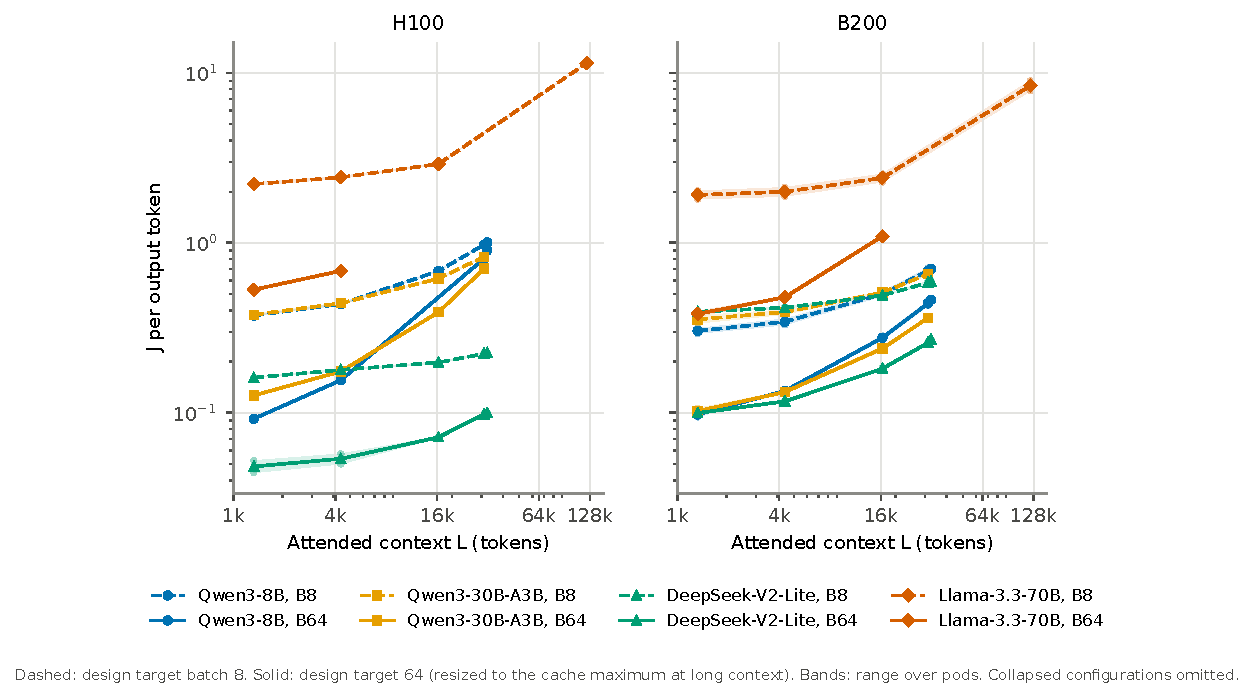
\includegraphics[width=\textwidth]{fig2_decode_context}
\caption{Energy per output token of the decode workload against context, experiment c2 (gross board energy including the idle draw). Dashed: design batch 8. Solid: design batch 64, cut at long context to what the cache could hold. Context counts the cached prefix, 200 fresh input tokens and half of the 256 output tokens. Points are runs, lines the mean and bands the range over pods. Collapsed configurations are omitted.}\label{fig:context}
\end{figure}

\begin{figure}[t]
\centering
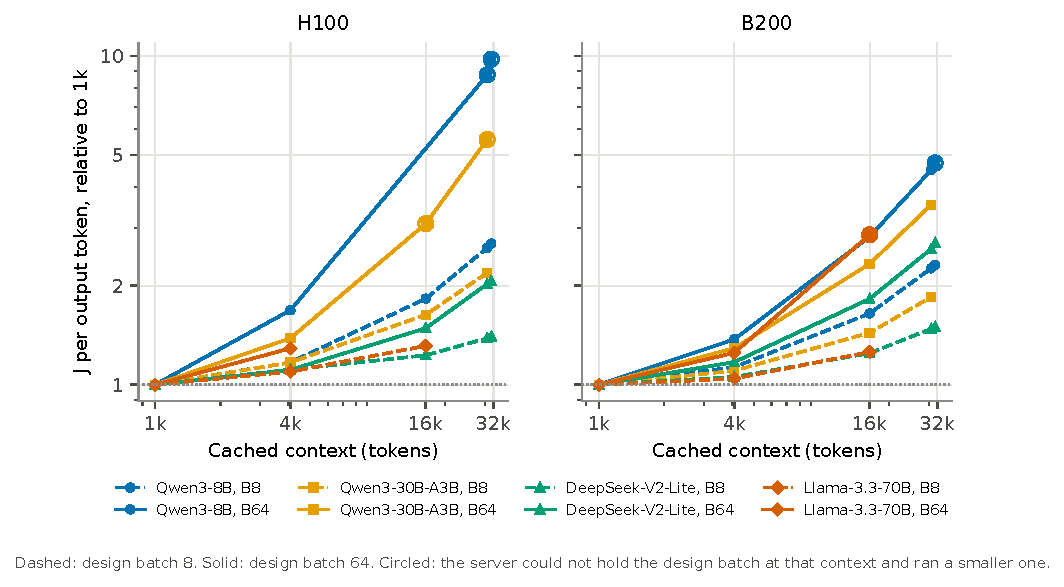
\includegraphics[width=\textwidth]{fig_context_multiplier}
\caption{The context multiplier: energy per output token at each cached context over the same configuration at 1k, experiment c2. Dashed: design batch 8. Solid: design batch 64. Circled points: the cache could not hold the design batch, so the server ran a smaller one and the rise includes that. Ratios of central values, without bands (Table~\ref{tab:decode_context} gives them).}\label{fig:ctxmult}
\end{figure}

\subsection{Energy per prompt token, with prefix caching off}\label{sec:prefill}

Reading a prompt cost far less per token than writing an answer (Figure~\ref{fig:prefill}, Table~\ref{tab:prefill}). The three smaller models used 0.011 to 0.029 J per prompt token, with one exception discussed below, and Llama-3.3-70B 0.074 to 0.18 J up to 16k and 0.17 to 0.27 J at 125k. That is roughly a thirtieth to a twelfth of the decode workload's energy per output token at batch 8 (ratios of central values). Each prefill request also wrote one output token. Concurrency mattered less than for decode, because prefill already sends every prompt token through the weights together: eight concurrent requests cut the 1k-prompt figure by 3 to 56\% (26\% for Llama-3.3-70B on both GPUs), and by less at long prompts. For Llama-3.3-70B the cost per token rose with prompt length, from 0.100 [0.095, 0.105] at 1k to 0.170 [0.166, 0.175] at 125k (B200, one request at a time), because attention's work grows with the square of the prompt length, which adds a cost per token that grows in proportion to the length on top of the fixed cost of reading the weights. For the MoE models it was flat or slightly lower up to 16k. Prefill windows drew 34 to 99\% of rated board power, more at long prompts than any decode window (35 to 93\%), in line with \citet{patel2024power}.

Two prefill results need care. First, prefill varied most between pods. For DeepSeek-V2-Lite and Qwen3-30B-A3B reading 1k-token prompts one at a time on B200, the two pods differed by a factor of 1.7 to 2.2 (0.018 to 0.040 and 0.020 to 0.033 J per token), and across the experiment the two runs of one configuration in ten differed by 24\% or more. Short-prompt prefill figures are ranges, not points. Second, Qwen3-8B on B200, the exception above, cost 0.039 to 0.047 J per prompt token up to 16k and about half that, 0.018 to 0.025 J, at its longest prompts (31.2k to 32.5k), on both pods. The server read more than twice as many prompt tokens per second at the same power. The exception was one request at a time at 31.2k, which still cost 0.047 [0.045, 0.050] J per token. We do not know why the server read faster at the longest prompts. Testing lengths between 16k and 31k would show where the change begins.

\begin{figure}[t]
\centering
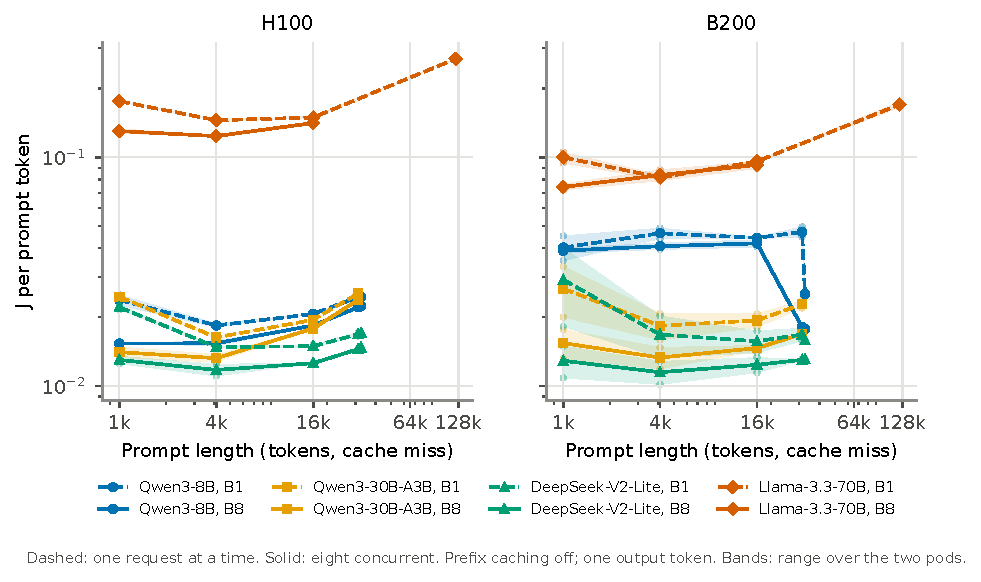
\includegraphics[width=\textwidth]{fig3_prefill}
\caption{Prefill energy per prompt token with prefix caching off, experiment c3 (gross board energy including the idle draw, prefix caching off, one output token). Dashed: one request at a time. Solid: eight concurrent. Points are runs, lines the mean and bands the range over pods.}\label{fig:prefill}
\end{figure}

\subsection{Cached prefix against uncached control}\label{sec:cached}

A cached prefix saved up to 84\% of a request's energy, and the saving grew with the cached length and with batch concurrency (Figure~\ref{fig:cached}, Table~\ref{tab:cached}). Each comparison sets a request whose first 1k, 4k or 16k tokens were already in the server's cache, followed by 200 or 2,048 fresh tokens and a 200-token answer, against a control of the same length sent entirely fresh. Filling the cache was outside the window. As the median ratio of cached to uncached energy, over models, GPUs and the two concurrencies, with the smallest and largest in brackets:
\begin{itemize}
\item 1k cached: 0.91 (0.64 to 0.98);
\item 4k cached: 0.68 (0.31 to 0.91);
\item 16k cached: 0.39 (0.165 to 0.67).
\end{itemize}
The largest saving was DeepSeek-V2-Lite on H100 at 16k cached, 200 fresh and eight concurrent, at 0.1651 [0.1648, 0.1653]. The saving was smaller at one request at a time, where the idle floor is a larger share of each request's energy and reading the cache is not free. At 1k cached, 15 of the 16 combinations lay between 0.92 and 0.98, and one band reaches 1.0.

\begin{figure}[t]
\centering
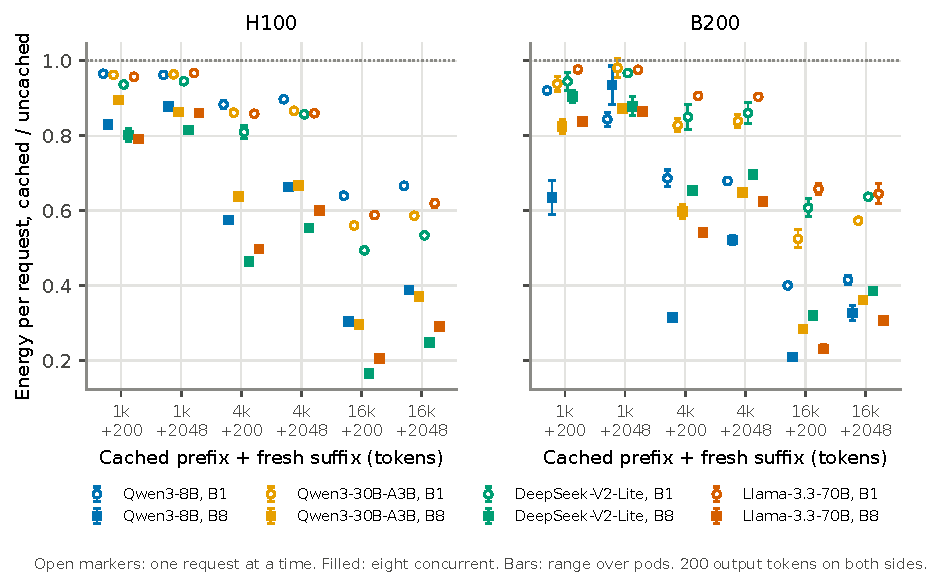
\includegraphics[width=\textwidth]{fig4_cached_prefix}
\caption{Cached-prefix access, experiment c4: energy per completed request with a warm cached prefix over a matched uncached control of the same total length (gross board energy, 200 output tokens on both sides). Columns: GPU. Rows: fresh suffix of 200 or 2,048 tokens. Dashed lines: one request at a time. Solid lines: eight concurrent. Bars: range over pods, paired by pod where both sides share pods.}\label{fig:cached}
\end{figure}

\subsection{Tensor parallelism}\label{sec:tp}

Tensor parallelism splits each layer of a model across GPUs that compute together and exchange results at every layer. Operators use it when a model does not fit on one GPU, as for Llama-3.3-70B on H100, or to answer each request faster. We measured its energy cost when the model would fit on fewer GPUs. Every split raised throughput and cost 7 to 40\% more energy per token (Figure~\ref{fig:tp}, Table~\ref{tab:tp}). Two causes are plausible, and we did not separate them: each added GPU brings its own idle draw (Section~\ref{sec:idle}), and the GPUs spend part of each step exchanging results.
\begin{itemize}
\item Qwen3-8B, one H100 to two: 1.27 [1.26, 1.28] to 1.371 [1.371, 1.372] times the energy per token, for 1.30 to 1.31 times the throughput (paired by pod).
\item Qwen3-8B, one B200 to two: 1.07 [1.06, 1.08] at batch 64 to 1.40 [1.33, 1.48] at batch 1, for 1.12 to 1.42 times the throughput (two-GPU side on one pod).
\item Llama-3.3-70B, two H100s to four: 1.07 [1.03, 1.11] to 1.09 [1.08, 1.10], for 1.51 to 1.53 times the throughput (four-GPU side on one pod).
\item Llama-3.3-70B on B200: one GPU to two cost 1.13 times at every batch (bands 1.06 to 1.21), and two to four 1.149 [1.148, 1.149] to 1.23 [1.22, 1.23], each step giving 1.3 to 1.6 times the throughput (each side on one pod).
\end{itemize}
Throughput ratios are ratios of central values. The energy cost was highest at one request at a time and shrank as the batch grew, except for Llama-3.3-70B going from two B200s to four.

\subsection{Weight precision on B200}\label{sec:precision}

With the published 4-bit (nvfp4) versions of the models, energy per output token was 0.61 to 0.86 of the fp8 (8-bit) figure at the same design batch and context (Figure~\ref{fig:precision}, Table~\ref{tab:precision}): 0.65 [0.62, 0.68] to 0.74 [0.70, 0.79] for Llama-3.3-70B and 0.61 [0.60, 0.62] to 0.86 [0.83, 0.90] for Qwen3-8B. The saving was largest at batch 64 and 1k context and smallest at 16k context, where reading the stored context, which 4-bit weights do not shrink, is a larger share of each step. Throughput rose 1.5 to 1.7 times for the 70B model and 1.03 to 1.2 times for the 8B (ratios of central values). The Llama-3.3-70B configuration at 16k context and design batch 64 is absent: both servers were at the cache limit, and three of its four runs recomputed the cached context on every request (Appendix~\ref{app:tables}); version 1.0.0 listed it and excluded it from these ranges. The figures describe the tested deployments, not bit width alone. They rest on eight windows for Qwen3-8B and six for Llama-3.3-70B, from one pod each, use 4-bit versions made by third parties, make no adjustment for output quality, and gave the server 70\% of GPU memory rather than 90\%, so the deepest Qwen3-8B point reached 35 requests against 53 at fp8.

\begin{figure}[t]
\centering
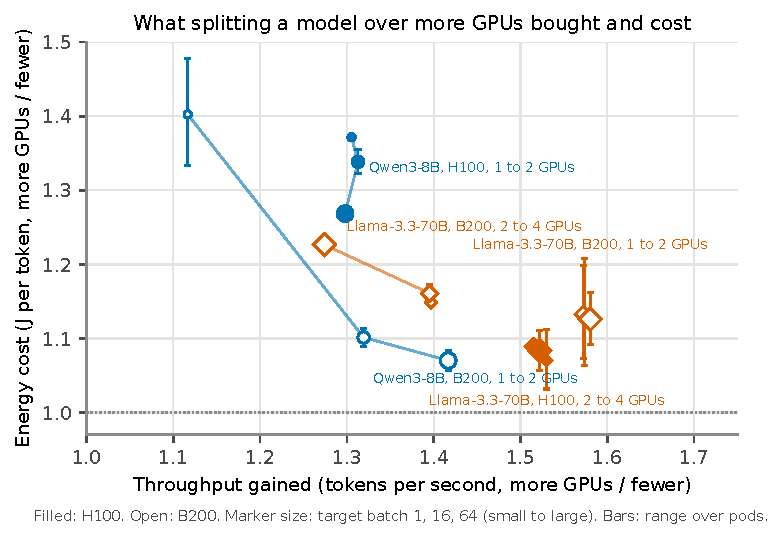
\includegraphics[width=0.8\textwidth]{fig_tp}
\caption{Tensor parallelism, experiment c6: the throughput gained (horizontal) and the energy per output token paid (vertical) by moving to the next larger number of GPUs, at target batch 1, 16 and 64 (marker size). Both axes are ratios, more GPUs over fewer. Every point lies above 1 on the vertical axis, so every split cost energy. Filled markers: H100. Open: B200. Bars: range over pods.}\label{fig:tp}
\end{figure}

\begin{figure}[t]
\centering
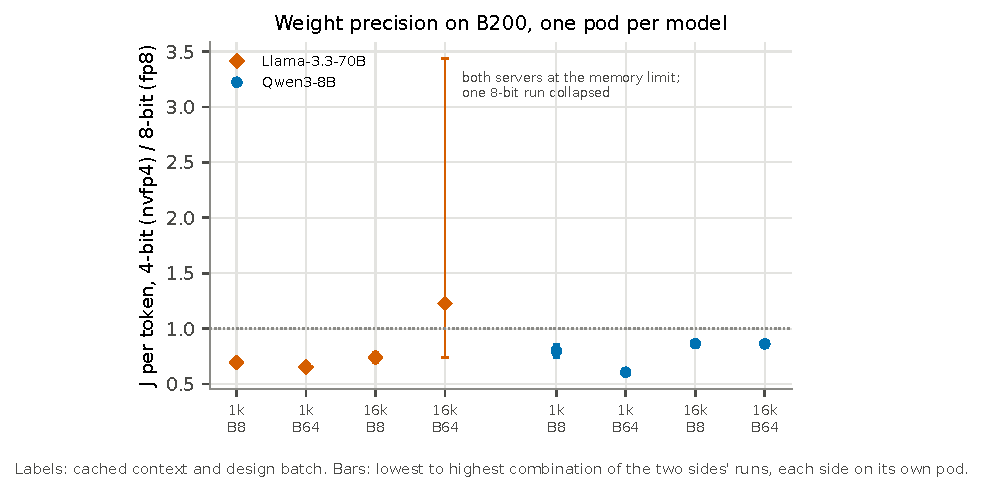
\includegraphics[width=0.75\textwidth]{fig_precision}
\caption{Weight precision on B200, experiment c7: energy per output token with 4-bit (nvfp4) weights over 8-bit (fp8), at the same design batch and cached context, one pod per model. Bars: lowest to highest combination of the two sides' runs. The very wide bar (Llama-3.3-70B, 16k context, batch 64) is not a property of 4-bit weights: both servers were at the cache limit and one 8-bit run collapsed (Section~\ref{sec:kv}). The text excludes that row.}\label{fig:precision}
\end{figure}

\subsection{Simulated agentic workload}\label{sec:agent}

A simulated agent cost 4.4 to 179 kJ run alone, and 2.4 to 3.7 times less per agent when several ran together (Table~\ref{tab:agent}, ratios of central values). An agent is a program that calls the model many times in a row, each time sending the whole conversation so far plus some new material. Each call is a step. A simulated agent sends a fixed script of such calls, and no real agent ran.

The workload reproduces what sets agentic use apart from chat: a long context that grows every step and is sent again each time, mostly from cache; a fresh block per step standing for a tool's output; short answers; and an occasional step whose cache is lost. The numbers are our choice, not fitted to real agents, which vary widely: a 10,240-token start, 2,048 tokens added and 300 written per step, and an uncacheable step at step 5. We intended one every fifth step, but a fault in the harness left step 5 as the only one (Appendix~\ref{app:detail}). The workload therefore shows the mechanism and its size, not a typical agent. The agents ran 30 steps on Llama-3.3-70B, reaching 69,632 tokens of context, and 11 steps on the three 32k-context models, reaching 30,720.

Run alone, an agent cost 4.4 to 11 kJ on the smaller models (0.40 to 1.0 kJ per step) and 150 [143, 158] kJ for Llama-3.3-70B on one B200 (5.0 [4.8, 5.3] kJ per step) or 179 [178, 180] kJ on two H100s. With five to eight agents in flight (seven for the 70B model on B200, five on two H100s), each agent cost 40.3 [38.6, 42.0] kJ for the 70B model on B200 and 1.4 to 3.5 kJ for the smaller models. Per output token, the simulated agents cost 1.3 to 20 J alone and 0.4 to 7.1 J together.

With several agents in flight, each output token cost 1.9 to 3.5 times (median 2.6) the energy per output token of the short-context reference workload on the same model and GPU (decode at 1k cached context and design batch 8, Table~\ref{tab:decode_context}), because every step pays again to read its context. The two workloads also differ in concurrency and step length, so this shows what re-reading a long context can do for a workload of this shape. It is not a general multiplier between agentic and chat use.

\subsection{KV-cache pressure}\label{sec:kv}

Running more requests at once lowers the cost of each token (Section~\ref{sec:batch}), up to the capacity of the KV-cache pool. Operators keep some headroom below it for latency, admission control and requests of varying length. This section shows what happened when a server went past it: Llama-3.3-70B on one B200 lost three-quarters or more of its throughput while its power rose 10 to 22\% (Table~\ref{tab:kv}). Experiments c9 and c9b raised the batch step by step at 16,384 tokens of cached context.
\begin{itemize}
\item Up to an achieved batch of 27, no run collapsed: 1.68 to 1.06 J per token, 452 to 783 tokens per second and 754 to 847 W, with the cache 36 to 89\% full on average and no requests waiting; the prefix cache served every cached token (reuse 1.00 in Table~\ref{tab:kv}).
\item At a target of 31, with the standard 90\% of memory offered, the server reached a batch of 23 and collapsed: 6.31 J per token, 147 tokens per second and 931 W, with the cache serving only 0.06 of the expected cached tokens. A diagnostic repeat at a target of 32 reached 25.6 and sat between the two states (2.18 J per token, 412 tokens per second, reuse 0.71).
\item With 70\% of memory offered, every target of 20 and above collapsed at an achieved batch of 13 to 14 (6.9 to 7.2 J per token, 128 to 134 tokens per second, 913 to 917 W, reuse 0.00 to 0.01), while a target of 12 did not (reuse 1.00).
\end{itemize}
In a collapse, throughput dropped 3.4- to 5.3-fold while power rose by a tenth to a fifth, so energy per token rose 4.1- to 5.8-fold. Requests waited and, where the counter was recorded (c9b), 7 or 8 were preempted per window. The cache counters give the mechanism: in every collapsed run the prefix cache served almost none of the cached context, so each request paid a fresh 16k-token prefill, and the one partial case (reuse 0.71) sat between the regimes. Shrinking the pool moved the collapse point, which ties it to cache capacity rather than to the batch itself. All these runs come from one pod per experiment. The same eviction explains the four configurations that version 1.0.0 flagged in Table~\ref{tab:decode_context} and the largest run-to-run differences it reported; version 1.0.1 excludes such runs outside this experiment (Appendix~\ref{app:tables}).

\subsection{Variability}\label{sec:variability}

Repeated measurements agreed closely. With at most two runs per configuration, we measure agreement by how far the two runs differed, as a percentage of their mean (Table~\ref{tab:cv}).
\begin{itemize}
\item Decode, 154 configurations: a median 2.1\% and a 90th percentile of 8.9\%. Runs on two pods differed more (2.7\% and 10.0\%, 124 configurations) than runs on one pod (0.6\% and 1.6\%, 30). As the larger run over the smaller, the median was 1.02 and the 90th percentile 1.09.
\item Prefill varied most (median 4.8\%, 90th percentile 24.4\%), and the memory-limit series least (median 0.3\%).
\item At one request at a time, B200 runs varied more than H100 runs (median 9.3\% against 1.2\%, Table~\ref{tab:cv_batch}).
\item The largest differences are 17\% on H100 (a target of 64) and 14\% on B200 (a target of 4 to 8). Version 1.0.0 reported 120\% and 118\%, from pairs in which one run had recomputed its cached context on every request; those runs are excluded (Appendix~\ref{app:tables}).
\item The three H100 configurations at the highest load, both runs on one pod, differed by a median 0.3\% and at most 7.5\%. The eight idle configurations differed by a median 3.9\% between pods.
\end{itemize}
A stable meter can still carry a stable bias, so none of this is an accuracy figure.

Of the throttle-reason snapshots taken at window edges, 8\% on H100 and 7\% on B200 showed the board at its power limit, and none showed a thermal or hardware slowdown. A brief slowdown inside a window would not show. We do not know whether hosts were shared with other tenants.

\subsection{Comparing the factors}\label{sec:factors}

Table~\ref{tab:factors} and Figure~\ref{fig:factors} put every measured factor on one scale: how many times energy per token changed between two named settings, as a median over the models and GPUs, with the smallest and largest beside it. Each row comes from the subsection that measures the factor, over the range it tested. The factors interact and the experiments varied one or two at a time, so the rows cannot be multiplied together.

Batch concurrency was the largest lever we tested: a median 21-fold difference (14- to 42-fold) between one request at a time and the highest load we report. Three effects of two to six times come next: running past the memory limit for stored context (4.1 to 5.8 times, one model on one GPU), long context at a target batch of 64 (median 3.2 times, partly because long context forced a smaller batch), and a cached 16k-token prefix (median 2.5 times less energy, up to 6 times). Then come long context at batch 8 (median 1.7 times), the tested 4-bit deployments (1.35 times) and tensor parallelism (1.13 times). The ranges differ in width, so Table~\ref{tab:factors} also gives the two factors we varied over a range, batch and context, as a change per doubling: batch cut energy per token by a median 1.63 for each doubling of the achieved batch, over about six doublings, while context raised it by 1.11 per doubling at batch 8 and 1.30 at batch 64, over two to five. The newer GPU on the same number of GPUs had no single direction (median 0.93, from 0.75 to 2.7), while one B200 against the two H100s Llama-3.3-70B needed saved more (0.70 to 0.93). Most of these effects are large against the difference between two repeats, pooled over all configurations (median 1.02, 90th percentile 1.09). The smallest are not: the lowest tensor-parallel cost (1.07) and the B200's median against the H100 (0.93, or 1.08 inverted) fall within it. The pooled figure shows scale and is not a test for any one comparison: some comparisons have bands much narrower than it (1.06 to 1.08 for one of the two 1.07 tensor-parallel costs).

For anyone estimating the energy of a deployment they cannot meter, the assumed batch concurrency deserves the most care, followed by context and prefix reuse, which matter most for workloads that re-read long contexts. A newer GPU cannot be assumed to save energy on the same number of GPUs, and an estimate should count the GPUs a model needs on each generation.

\begin{landscape}
\begin{table}[p]
\centering
\footnotesize
\setlength{\tabcolsep}{4pt}
\caption{The measured factors compared on one scale. Effect is the multiplier on energy per output token (per request for the cached prefix) between the two settings named in the Comparison column, as a ratio of central values: the median over the model and accelerator combinations, with the smallest and largest in parentheses. Comparisons counts those combinations (and, for the cached prefix, prompt shapes and concurrencies). Each row restates figures from the section that measures the factor; the GPU-generation row is two-sided because the direction depends on the model, and the GPU-memory row is one model (Llama-3.3-70B). Repeat-to-repeat variation is shown for scale, with its 90th percentile in place of a range.}\label{tab:factors}
\begin{tabular}{>{\raggedright\arraybackslash}p{2.5cm}>{\raggedright\arraybackslash}p{6.0cm}lr>{\raggedright\arraybackslash}p{2.7cm}>{\raggedright\arraybackslash}p{4.9cm}}
\toprule
Factor & Comparison & \makecell[l]{Effect, median\\(range)} & \makecell[r]{Compar-\\isons} & \makecell[l]{Per\\doubling} & What the data tell us \\
\midrule
Batch & one request at a time over the deepest batch & 20.7 (13.6 to 42.3) & 8 & 1.63 (1.49 to 1.78) & the dominant lever on every model and both GPUs \\
Cached prefix & fresh request over one with 16k tokens already cached & 2.54 (1.5 to 6.06) & 32 & -- & large for long reused prompts, small (median 9\%) at 1k \\
Memory limit for stored context & past the limit over just below it (Llama-3.3-70B, one B200) & 4.29 (4.11 to 5.84) & 5 & -- & a cliff, not a slope: admission limits and memory headroom reduce the risk, but the safe point depends on the workload and the scheduler \\
Context length, batch 64 & longest context whose runs kept their cache (4k for Llama-3.3-70B on H100, 16k on B200, 31k to 32k for the others) over 1k, design batch 64; long context forced a smaller batch on some servers & 3.19 (1.29 to 9.79) & 8 & 1.30 (1.14 to 1.58) & rises with context and more steeply at deep batch, where the stored context fills memory \\
Context length, batch 8 & longest context (16k to 32k) over 1k, design batch 8 & 1.67 (1.26 to 2.69) & 8 & 1.11 (1.06 to 1.22) & a moderate, steady rise \\
GPU generation, same GPU count & B200 over H100 on the same number of GPUs, at the same batch & 0.929 (0.753 to 2.7) & 24 & -- & no consistent saving: lower for some models, higher for DeepSeek-V2-Lite \\
One B200 against two H100s & one B200 over the two H100s Llama-3.3-70B needs, at the same batch; changes GPU generation and GPU count together, and at the highest load also the cache reuse & 0.855 (0.702 to 0.927) & 4 & -- & a saving because the larger memory holds the model on fewer GPUs \\
Weight precision & 8-bit over 4-bit weights, B200 (one pod per model) & 1.35 (1.16 to 1.64) & 7 & -- & a modest saving in the tested 4-bit deployments; one pod, so indicative \\
Tensor parallelism & a model split over more GPUs over fewer & 1.13 (1.07 to 1.4) & 15 & -- & costs energy; buys throughput \\
Repeat-to-repeat variation & the larger over the smaller of two repeats & 1.02 (90th percentile 1.09) & 154 & -- & small against most of the levers above, though not against the smallest \\
\bottomrule
\end{tabular}
\end{table}
\end{landscape}


\begin{figure}[t]
\centering
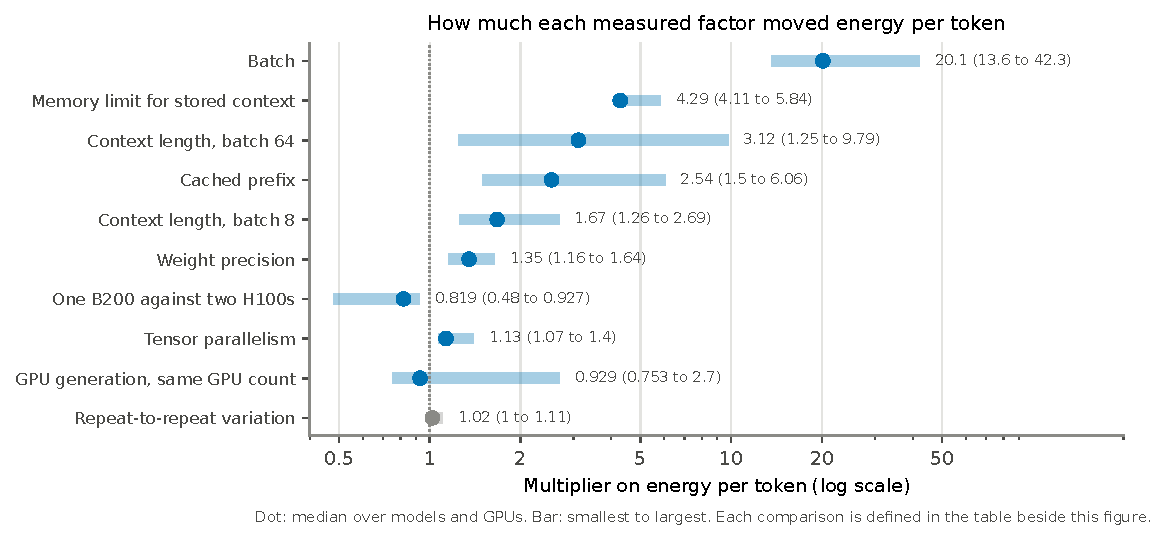
\includegraphics[width=\textwidth]{fig_factors}
\caption{How much each factor moved energy per token over the ranges tested (log scale). Dot: median over the model and GPU combinations. Bar: smallest to largest. Table~\ref{tab:factors} defines each comparison. All values are ratios of central values from Sections~\ref{sec:batch} to \ref{sec:variability}. Grey: the difference between two repeats (larger over smaller), shown for scale, with its 90th percentile as the upper end.}\label{fig:factors}
\end{figure}

\section{Limitations}\label{sec:threats}

Eight things limit how far these figures travel.

\paragraph{Rented pods.} We rented the pods and did not control them, and the container would not let us lock the clocks. For the 413 configurations run on two pods, the band is the spread between pods, and so includes the effect of these uncontrolled conditions. For the 59 run on one pod, the band is only the range of the repeats and may understate the spread. These include the H100 runs at the highest load, the larger tensor-parallel configurations, the 4-bit runs and the memory-limit series. Four pods, two per accelerator, supplied 91\% of the runs (Table~\ref{tab:pods}). The records carry the marketplace's pod identifiers, not hardware serial numbers, so we cannot confirm that the 13 pods were 13 distinct physical servers.

\paragraph{Power sampling and the counter.} We established how often the board's readings update, but not the interval they average over or how accurate they are (Section~\ref{sec:power}). The counter and the sampled power agree, but a bias shared by both would not show. The counter includes the energy of short events, but neither reading shows how power varies within a second. That matters little for windows of 60 s or more, more at the edges of the shorter simulated-agent runs, and would matter for dividing energy among requests running at the same time. We did not measure the energy of the rest of the server (its CPUs, memory, fans and network).

\paragraph{Workload windows, not isolated phases.} A decode-workload window also includes reading each request's 200 fresh input tokens (prefill), and the server can process one request's prefill in the same step as another's decode. Our figures are therefore energy per output token of a stated workload, not the energy of the decode phase alone. We did not measure the fresh input's share, which may be largest at high load. Likewise, each prefill-workload request also wrote one token.

\paragraph{Gross energy and the idle floor.} A server busier than ours, or one that runs more models on each board, spreads the idle floor over more tokens. A server that sits idle most of the time spreads it over fewer. The right figure for a deployment therefore depends on its utilization, which we did not measure. The idle share we tabulate is a starting point for adjusting in either direction, but only for more or less idle time at the same batch: a busier server also tends to run larger batches, which changes energy per token as well (Section~\ref{sec:batch}).

\paragraph{Synthetic prompts and one serving stack.} The prompts are synthetic text of set lengths, while real traffic mixes many lengths and shapes. Every experiment ran on one version of one serving system with fixed settings. A different scheduler, set of kernels or attention implementation could move any figure, and we did not vary them. Three models ran from 8-bit versions that others had published, and vLLM converted DeepSeek-V2-Lite to 8-bit as it loaded it. The cache was fp8 throughout. A different conversion of the same model could move the figures. For the MoE models, random text may spread requests over the experts differently from natural text, which changes the weight bytes each step reads. The B200 figures also depend on how well this version's kernels used Blackwell: at one request neither GPU was near its bandwidth bound, and the B200 was further from it (Table~\ref{tab:roofline}).

\paragraph{nvfp4.} The 4-bit experiment rests on eight windows for Qwen3-8B and six for Llama-3.3-70B, each model on one pod. Its servers were offered less memory than the fp8 servers, and its 4-bit versions of the models were made by third parties. We therefore read its ratios (0.61 to 0.86) as describing those two versions, not 4-bit precision in general.

\paragraph{The highest load.} The load generator's 100-connection limit, not the GPU, set the highest load in the batch experiment, so the deepest points understate how far batching can go. On H100 that load ran on one pod only, so its band is the range of the repeats and may understate the spread between pods. Separately, some pods gave the server 12 to 56\% more memory for stored context than the harness predicted (from the server logs, not tabulated). This moved the point at which the long-context experiments reached the KV-cache boundary.

\paragraph{Batch as achieved.} The plotted batch is the server's mean count of running requests. It is not the client's desired concurrency, which includes requests waiting for a connection, nor exactly the number of requests advanced in any one step. It sits up to 18\% below the target at targets up to 64, and far below it at 256.

\section{Data and code availability}

\begin{sloppypar}
The corpus, the metering harness and the analysis script are deposited together on Zenodo (\href{https://doi.org/10.5281/zenodo.24014980}{doi:10.5281/\allowbreak zenodo.24014980}), and the code is maintained in the repository~\citep{harness2026}. The deposit holds:
\begin{itemize}
\item the corpus (\texttt{features.parquet}, one row per run, with the per-GPU window records and the raw power samples beside it) and its checksum;
\item the harness and analysis code at the commit that produced this paper;
\item the names and revisions of the model files we downloaded;
\item the command that rebuilds every table and figure, and a data dictionary stating what each field measures (the per-request cached-token field, for example, was not reported by the server and is stored as zero).
\end{itemize}
Re-running \texttt{analysis/build.py} on the corpus regenerates every table and figure and the numbers quoted from them. A few figures come instead from the per-window records and the server and qualification logs: the counter check (Appendix~\ref{app:detail}), the prefix-cache hit rates (Section~\ref{sec:batch}), the time to first token (Table~\ref{tab:latency}, from the per-request records, by \texttt{analysis/latency.py}), the driver version (Section~\ref{sec:method_pods}) and the memory-pool sizes (Section~\ref{sec:threats}). The code is licensed under Apache 2.0 and the corpus under CC BY-NC 4.0, with express permission for use by regulators, standards bodies and public authorities and for verification by auditors. The text is CC BY-NC-ND 4.0 in its preprint versions. Appendix~\ref{app:license} gives the terms.
\end{sloppypar}

\paragraph{Declarations.}

\noindent\emph{Copyright and Licensing.} \textcopyright{} 2026 InferenceCarbon Ltd. Code: Apache 2.0; corpus: CC BY-NC 4.0, with express permission for regulators, standards bodies, public authorities and auditors; text: CC BY-NC-ND 4.0 in its preprint versions. Appendix~\ref{app:license} gives the full terms.

\noindent\emph{Use of AI.} AI assistants (Anthropic's Claude models) were used under the author's direction to write the metering harness and the analysis script, to check results against the corpus, and to draft and revise text. The author set the research questions and the experimental design, reviewed every section, table and figure in repeated, detailed rounds against the data, decided every revision, and takes full responsibility for the paper's content and conclusions. Every table and figure is generated by the published analysis script from the deposited corpus, so each can be checked independently.

\noindent\emph{Funding.} InferenceCarbon Ltd paid for the work, including the rented GPU time, bought at the marketplace's published rates. No GPU vendor, cloud provider or model developer funded, supplied or reviewed the work.

\noindent\emph{Competing interests.} The author is the founder of InferenceCarbon Ltd, which publishes and sells estimates of the energy and emissions of AI use that draw on measurements such as these.

\noindent\emph{Data.} The work studied no human participants and contains no personal data.

\bibliographystyle{IEEEtranN}
\bibliography{refs}

\appendix

\section{The experiments}\label{app:cells}

See Figure~\ref{fig:experiments}: each experiment is a set of runs designed to answer one question, such as how energy per token changes with batch size. Table~\ref{tab:cells} lists the ten experiments. For each it gives the kind of work measured, the settings that were varied (each combination of them, for each model and GPU, is one configuration) and the settings held fixed.

All experiments followed the same procedure. Each run metered one workload, after up to four warm-up requests that were not metered (one at a target batch of one, and none in the idle and simulated-agent experiments). The load workloads (c1 to c4, c6, c7, c9 and c9b) issued requests until the window reached at least 60 seconds and 20,000 tokens, then let the requests in flight finish. The idle experiment (c0) metered a fixed 60 s. The simulated agent (c8) metered one complete run of its script, which lasted 16 to 375 s. Its per-token figures count output tokens only, although each step also read up to 69,632 prompt tokens. The idle power of the GPU was measured for 60 seconds before and after each window, and a run whose two idle readings differed by more than 5\% was flagged. Requests used temperature 0 and a fixed seed. Unless the table says otherwise, each configuration ran twice, with 8-bit (fp8) weights and stored context.

``Native max'' is the longest context the model allows, less the answer, the fresh input and a safety margin of 256 tokens plus 4\%. We tightened the margin during the measurements, so the 32k-context models have two native-max points: 30,745 and 32,056 tokens for decode, and 31,200 and 32,511 for prefill. Four decode runs and four prefill runs at exactly 32,768 tokens failed, every request refused by the server's context limit. These appear in no results table.

\begin{table}[h]
\centering
\caption{The ten experiments. Each row is one experiment: its label in the deposited data, the workload it measured (decode: decode-oriented requests whose window also reads their fresh input; prefill: cache-miss prompts with one output token), the settings it varied and the settings it held fixed. Batch is the number of requests the server ran at once; context is the number of tokens of earlier text the model reads back; ``fresh'' is the number of new input tokens per request and ``out'' the number of tokens in the answer. TP is the number of GPUs sharing one model.}\label{tab:cells}
\begin{footnotesize}
\setlength{\tabcolsep}{4pt}
\begin{tabular}{ll>{\raggedright\arraybackslash}p{5.8cm}>{\raggedright\arraybackslash}p{3.8cm}}
\toprule
Experiment & Workload & Varied & Fixed \\
\midrule
c0\_static & idle, loaded & -- & fixed 60 s window, default clocks \\
c1\_decode\_batch & decode & target batch 1, 4, 16, 64, 256 (at 256, at most 100 ran at once) & cached context 1,024; fresh 200; out 256 \\
c2\_decode\_context & decode & cached context 1k, 4k, 16k, native max; target batch 8, 64 & fresh 200; out 256 \\
c3\_prefill\_miss & prefill & fresh prompt 1k, 4k, 16k, native max; target batch 1, 8 & prefix caching off; out 1 \\
c4\_cached\_prefix & prefix access & cached prefix 1k, 4k, 16k; fresh 200, 2,048; target batch 1, 8; control cached or uncached (same total length, all fresh) & out 200 \\
c6\_tensor\_parallel & decode & TP 1, 2 (Qwen3-8B), 2, 4 (Llama-3.3-70B); target batch 1, 16, 64 & cached context 1,024; fresh 200; out 256 \\
c7\_precision & decode & weight precision fp8, nvfp4; target batch 8, 64; cached context 1k, 16k & B200 only; fresh 200; out 256 \\
c8\_agent\_replay & composite & agents in flight 1, 8 (8 resized to 7 and 5 for the 70B model) & one complete script; 30 steps (11 on the 32k-context models); context 10,240 + 2,048 per step, capped at the window; 300 out per step; cache misses at steps 1 and 5 only (Appendix~\ref{app:detail}) \\
c9\_kv\_pressure & decode & target batch 12, 16, 20, 24, 28, 32 & Llama-3.3-70B, B200; cached context 16,384; fresh 200; out 256 \\
c9b\_kv\_pressure\_diag & decode & target batch 12, 20, 28, 32; GPU memory offer 0.9, 0.7; one repeat & as c9, with the preemption counter recorded \\
\bottomrule
\end{tabular}
\end{footnotesize}
\end{table}

We designed a clock-sweep experiment (c5) but withdrew it because the container would not let us lock the clocks.

\section{Corpus}\label{app:corpus}

\newgeometry{margin=0.6in}
\begin{landscape}
\begin{table}[t]
\centering
\scriptsize
\setlength{\tabcolsep}{3pt}
\caption{Metered runs per experiment, model and accelerator (917 runs).}\label{tab:corpus}
\begin{tabular}{lrrrrrrrrr}
\toprule
Experiment & \makecell[r]{H100\\Qwen3-8B} & \makecell[r]{H100\\Qwen3-30B-A3B} & \makecell[r]{H100\\DeepSeek-V2-Lite} & \makecell[r]{H100\\Llama-3.3-70B} & \makecell[r]{B200\\Qwen3-8B} & \makecell[r]{B200\\Qwen3-30B-A3B} & \makecell[r]{B200\\DeepSeek-V2-Lite} & \makecell[r]{B200\\Llama-3.3-70B} & Total \\
\midrule
c0\_static & 2 & 2 & 2 & 2 & 2 & 2 & 2 & 2 & 16 \\
c1\_decode\_batch & 10 & 10 & 10 & 10 & 10 & 10 & 10 & 10 & 80 \\
c2\_decode\_context & 22 & 16 & 18 & 14 & 22 & 16 & 19 & 14 & 141 \\
c3\_prefill\_miss & 22 & 16 & 18 & 16 & 22 & 16 & 18 & 16 & 144 \\
c4\_cached\_prefix & 48 & 48 & 48 & 48 & 48 & 48 & 48 & 48 & 384 \\
c6\_tensor\_parallel & 12 & 0 & 0 & 12 & 12 & 0 & 0 & 12 & 48 \\
c7\_precision & 0 & 0 & 0 & 0 & 16 & 8 & 8 & 16 & 48 \\
c8\_agent\_replay & 6 & 4 & 4 & 4 & 6 & 4 & 4 & 4 & 36 \\
c9\_kv\_pressure & 0 & 0 & 0 & 0 & 0 & 0 & 0 & 12 & 12 \\
c9b\_kv\_pressure\_diag & 0 & 0 & 0 & 0 & 0 & 0 & 0 & 8 & 8 \\
Total & 122 & 96 & 100 & 106 & 138 & 104 & 109 & 142 & 917 \\
\bottomrule
\end{tabular}
\end{table}
\end{landscape}
\restoregeometry

\begin{table}[t]
\centering
\footnotesize
\setlength{\tabcolsep}{4pt}
\caption{The 13 rented pods. Pod identifiers are replaced by an index (the mapping is in the deposited corpus). Metered hours are the summed lengths of the metered windows on that pod, warm-up, idle windows and model loads excluded.}\label{tab:pods}
\begin{tabular}{lrrrrrr}
\toprule
Pod & Data center & Accelerator & GPUs & \makecell[r]{Models\\(count)} & Runs & \makecell[r]{Metered\\hours} \\
\midrule
pod 1 & US-CA-2 & B200 & 1 & 4 & 220 & 4.63 \\
pod 2 & US-NC-2 & B200 & 1 & 4 & 218 & 5.66 \\
pod 3 & US-TX-6 & B200 & 1 & 1 & 12 & 0.28 \\
pod 4 & EU-RO-1 & B200 & 2 & 2 & 12 & 0.33 \\
pod 5 & US-NC-2 & B200 & 1 & 1 & 8 & 0.14 \\
pod 6 & US-NC-2 & B200 & 1 & 1 & 8 & 0.26 \\
pod 7 & US-NC-2 & B200 & 1 & 1 & 8 & 0.17 \\
pod 8 & US-NE-1 & B200 & 4 & 1 & 6 & 0.18 \\
pod 9 & US-NC-2 & B200 & 1 & 1 & 1 & 0.02 \\
pod 10 & US-MO-1 & H100 & 2 & 4 & 201 & 5.31 \\
pod 11 & AP-IN-1 & H100 & 2 & 4 & 198 & 6.93 \\
pod 12 & US-MO-1 & H100 & 2 & 4 & 19 & 0.44 \\
pod 13 & CA-MTL-1 & H100 & 4 & 1 & 6 & 0.19 \\
\bottomrule
\end{tabular}
\end{table}


\begin{sloppypar}
The two corpus files are frozen. Their SHA-256 checksums are \texttt{1a186b92\allowbreak 9cf09b60\allowbreak da5dec06\allowbreak 020fa6a0\allowbreak c1498ae1\allowbreak 42ecdaff\allowbreak bf765d03\allowbreak 1981abaf} (\texttt{features.parquet}) and \texttt{4b11fa45\allowbreak d691bc53\allowbreak a20204c8\allowbreak a3983eca\allowbreak 4e758faa\allowbreak ed49053a\allowbreak de908747\allowbreak 043d675a} (\texttt{store\_tables/cells.parquet}); the deposit's checksum list covers the raw records.
\end{sloppypar}

\section{Full tables}\label{app:tables}

These conventions apply to every table in this appendix. ``J per output token'' and ``J per prompt token'' are gross board energy, including the idle draw and summed over the GPUs sharing the model, divided by the output or prompt tokens of the requests in the window. TP is the tensor-parallel degree. Brackets give the range over the two pods, or the range of the repeats where there was one pod, and a single run is marked n=1. The Pods column gives the number of pods behind each row. Ratio tables give the pods on each side and whether the ratio was paired. Throughput columns are means over runs, with no band.

We tabulate every configuration with at least one usable run, with five exceptions:
\begin{itemize}
\item the fp8-only c7 runs of the two MoE models (16 runs), for which we had no 4-bit version to compare with;
\item the two early Qwen3-8B simulated-agent runs per accelerator with a 32,768 context cap (4 runs, one run each), superseded by the 31,744-cap configuration;
\item four c3 prefill runs at a 32,768-token prompt, every request of which was refused;
\item the four c2 decode runs at 32,768 cached context, which have no usable window;
\item eleven decode runs whose cached context was recomputed on most requests (version 1.0.1; see below): Llama-3.3-70B on two H100s at a target of 256 (both runs) and at 16k context and a target of 64 (both); Qwen3-8B on H100 at 16k and a target of 64 (both); Llama-3.3-70B on B200 at 16k and a target of 64 (one c2 run, one fp8 c7 run and both nvfp4 c7 runs); and one Llama-3.3-70B run on two H100s at 125k context and a target of 8.
\end{itemize}
Five Llama-3.3-70B prefill configurations on H100 appear with n=1 because the second run lacks a prompt-token count, and three decode configurations because the other run is among the eleven above.

\paragraph{Cache-reuse check (version 1.0.1).} The harness that collected this corpus confirmed that each request's cached prefix was in the server's cache before the window, but did not check that it stayed there during the window. The server's prefix-cache counters, recorded for every window, allow that check to be made after the fact. For each run we divide the share of prompt tokens the server found in its cache during the window by the share that was meant to be cached (the cached context over the cached context plus the fresh input). A value of 1 means the cache held throughout the window, and a value near 0 means the server evicted the prefixes and recomputed the context on almost every request. The value is an average over the window (\path{data/cache_reuse.csv}).

Of the 529 runs with a cached context, 523 recorded the counters. Their values fall into two clear groups: 504 runs at 0.97 or above, and 17 at 0.85 or below. Two runs lie between, at 0.957 and 0.962: Qwen3-8B on H100 at 32k context, design target 64, run at 25, the 9.8-fold point of Section~\ref{sec:context}. We keep them, noting that about 4\% of their context was recomputed per request.

Version 1.0.1 excludes decode runs (experiments c1, c2, c6 and c7) below 0.95, a cut that sits in the gap between the two groups, because those runs did not perform the cached-context workload their configuration states. The KV-pressure runs (c9 and c9b) keep theirs, since eviction is what those experiments measure, and Table~\ref{tab:kv} prints the value. Excluded runs stay in the corpus file with the reason recorded. We developed this check for the replication campaign that followed this paper, where the same fault appeared, and then applied it to this corpus.

\begin{table}[t]
\centering
\footnotesize
\setlength{\tabcolsep}{4pt}
\caption{Loaded-idle board power (experiment c0: model loaded, no requests, default power management, 60 s window), summed over the GPUs serving the model. Mean over runs, with the range over the two pods in brackets. Share of rated: W per GPU over 700 W (H100) or 1,000 W (B200).}\label{tab:idle}
\begin{tabular}{llrrrrr}
\toprule
Model & Accelerator & GPUs & \makecell[r]{Board W, all\\GPUs} & W per GPU & \makecell[r]{Share of\\rated} & Pods \\
\midrule
DeepSeek-V2-Lite & B200 & 1 & 245 {[}239, 250{]} & 245 & 24\% & 2 \\
DeepSeek-V2-Lite & H100 & 1 & 127 {[}126, 129{]} & 127 & 18\% & 2 \\
Llama-3.3-70B & B200 & 1 & 244 {[}239, 249{]} & 244 & 24\% & 2 \\
Llama-3.3-70B & H100 & 2 & 259 {[}249, 270{]} & 130 & 19\% & 2 \\
Qwen3-30B-A3B & B200 & 1 & 245 {[}239, 250{]} & 245 & 24\% & 2 \\
Qwen3-30B-A3B & H100 & 1 & 123 {[}121, 125{]} & 123 & 18\% & 2 \\
Qwen3-8B & B200 & 1 & 244 {[}239, 249{]} & 244 & 24\% & 2 \\
Qwen3-8B & H100 & 1 & 124 {[}122, 126{]} & 124 & 18\% & 2 \\
\bottomrule
\end{tabular}
\end{table}

\begin{table}[t]
\centering
\footnotesize
\setlength{\tabcolsep}{4pt}
\caption{Idle share of decode power in the batch experiment (c1: 1k cached context, 200 fresh input and 256 output tokens). For each run, the board power the pod drew while idle with the model loaded, the mean of the 60 s idle windows before and after the run, divided by the mean board power of its decode window. Gross energy per token includes this share. Median, minimum and maximum over the runs of all four models at each target batch. No band, because each value is a ratio of two means from the same run.}\label{tab:idle_share}
\begin{tabular}{lrll}
\toprule
Accelerator & Target B & \makecell[l]{Idle share\\of board\\power,\\median} & min to max \\
\midrule
B200 & 1 & 57\% & 35\% to 68\% \\
B200 & 4 & 50\% & 34\% to 59\% \\
B200 & 16 & 40\% & 32\% to 46\% \\
B200 & 64 & 34\% & 28\% to 41\% \\
B200 & 256 & 35\% & 26\% to 46\% \\
H100 & 1 & 39\% & 27\% to 51\% \\
H100 & 4 & 34\% & 26\% to 47\% \\
H100 & 16 & 30\% & 23\% to 44\% \\
H100 & 64 & 24\% & 20\% to 37\% \\
H100 & 256 & 23\% & 23\% to 30\% \\
\bottomrule
\end{tabular}
\end{table}

\newgeometry{margin=0.6in}
\begin{landscape}
\begingroup
\scriptsize
\setlength{\tabcolsep}{3pt}
\begin{longtable}{llrrrrlllrr}
\caption{Energy per output token of the decode workload against batch (experiment c1: 1k cached context, 200 fresh input tokens, 256 output tokens; gross board energy including the idle draw). Target B is the number of requests the client kept in flight. Achieved B is the server's mean count of running requests over the middle 80\% of the window. At target 256 the client's HTTP connection pool (100 connections, the library default) let at most 100 requests stream at once, and the server ran 67 to 91 on average, so that row is the highest load we offered, not the most the GPU could hold. Mean KV use: the server's mean KV-cache occupancy over the same part of the window. Board W is the mean board power over the window summed over the GPUs in the TP column, and \% of rated divides it by 700 W per H100 or 1,000 W per B200. Brackets: the range over the two pods (one pod: the range of the repeats). TP: tensor-parallel degree (GPUs sharing the model).}\label{tab:decode_batch}\\
\toprule
Model & Acc. & TP & Target B & Achieved B & Mean KV use & \makecell[l]{J per output\\token} & \makecell[l]{Tokens per\\second} & Board W & \% of rated & Pods \\
\midrule
\endfirsthead
\toprule
Model & Acc. & TP & Target B & Achieved B & Mean KV use & \makecell[l]{J per output\\token} & \makecell[l]{Tokens per\\second} & Board W & \% of rated & Pods \\
\midrule
\endhead
\bottomrule
\endfoot
DeepSeek-V2-Lite & B200 & 1 & 1 & 0.9 & 0\% & 1.48 {[}1.44, 1.52{]} & 248 {[}245, 251{]} & 368 {[}353, 382{]} & 37\% & 2 \\
DeepSeek-V2-Lite & B200 & 1 & 4 & 3.8 & 0\% & 0.602 {[}0.595, 0.609{]} & 752 {[}715, 789{]} & 452 {[}425, 480{]} & 45\% & 2 \\
DeepSeek-V2-Lite & B200 & 1 & 16 & 14.8 & 0\% & 0.258 {[}0.257, 0.258{]} & 2,272 {[}2,094, 2,450{]} & 585 {[}541, 630{]} & 59\% & 2 \\
DeepSeek-V2-Lite & B200 & 1 & 64 & 54.4 & 1\% & 0.0995 {[}0.097, 0.102{]} & 6,556 {[}6,069, 7,044{]} & 654 {[}589, 719{]} & 65\% & 2 \\
DeepSeek-V2-Lite & B200 & 1 & 256 & 77.3 & 1\% & 0.0804 {[}0.0803, 0.0806{]} & 7,419 {[}6,397, 8,441{]} & 597 {[}515, 678{]} & 60\% & 2 \\
DeepSeek-V2-Lite & H100 & 1 & 1 & 0.9 & 0\% & 1.05 {[}1.04, 1.06{]} & 252 {[}250, 254{]} & 264.7 {[}264.6, 264.9{]} & 38\% & 2 \\
DeepSeek-V2-Lite & H100 & 1 & 4 & 3.7 & 0\% & 0.298 {[}0.291, 0.304{]} & 898 {[}893, 903{]} & 267 {[}263, 272{]} & 38\% & 2 \\
DeepSeek-V2-Lite & H100 & 1 & 16 & 14.3 & 1\% & 0.0953 {[}0.0915, 0.099{]} & 3,066 {[}2,959, 3,172{]} & 292 {[}290, 293{]} & 42\% & 2 \\
DeepSeek-V2-Lite & H100 & 1 & 64 & 52.4 & 2\% & 0.0465 {[}0.0425, 0.0505{]} & 7,559 {[}6,790, 8,328{]} & 348 {[}343, 354{]} & 50\% & 2 \\
DeepSeek-V2-Lite & H100 & 1 & 256 & 84.0 & 3\% & 0.0659 {[}0.0635, 0.0684{]} & 6,242 {[}6,125, 6,359{]} & 411 {[}403, 419{]} & 59\% & 1 \\
Llama-3.3-70B & B200 & 1 & 1 & 1.0 & 0\% & 14.3 {[}13.4, 15.2{]} & 47.6 {[}47.4, 47.8{]} & 679 {[}640, 719{]} & 68\% & 2 \\
Llama-3.3-70B & B200 & 1 & 4 & 4.0 & 1\% & 3.81 {[}3.58, 4.04{]} & 182 {[}181, 183{]} & 693 {[}655, 731{]} & 69\% & 2 \\
Llama-3.3-70B & B200 & 1 & 16 & 15.5 & 4\% & 1.02 {[}0.964, 1.07{]} & 729 {[}725, 734{]} & 741 {[}699, 783{]} & 74\% & 2 \\
Llama-3.3-70B & B200 & 1 & 64 & 61.0 & 16\% & 0.38 {[}0.368, 0.391{]} & 2,256 {[}2,216, 2,296{]} & 857 {[}816, 898{]} & 86\% & 2 \\
Llama-3.3-70B & B200 & 1 & 256 & 90.7 & 23\% & 0.338 {[}0.333, 0.342{]} & 2,744 {[}2,689, 2,799{]} & 927 {[}895, 958{]} & 93\% & 2 \\
Llama-3.3-70B & H100 & 2 & 1 & 1.0 & 0\% & 15.4 {[}15.1, 15.7{]} & 60.3 {[}60.0, 60.6{]} & 928 {[}916, 940{]} & 66\% & 2 \\
Llama-3.3-70B & H100 & 2 & 4 & 3.9 & 1\% & 4.27 {[}4.17, 4.38{]} & 228 {[}226, 229{]} & 974 {[}956, 991{]} & 70\% & 2 \\
Llama-3.3-70B & H100 & 2 & 16 & 15.6 & 6\% & 1.24 {[}1.23, 1.24{]} & 841 {[}841, 842{]} & 1,043 {[}1,040, 1,046{]} & 75\% & 2 \\
Llama-3.3-70B & H100 & 2 & 64 & 60.0 & 21\% & 0.541 {[}0.532, 0.55{]} & 2,300 {[}2,282, 2,318{]} & 1,245 {[}1,234, 1,255{]} & 89\% & 2 \\
Llama-3.3-70B & H100 & 2 & 256 & 82.7 & 30\% & 0.703 {[}0.699, 0.708{]} & 1,883 {[}1,877, 1,889{]} & 1,325 {[}1,321, 1,329{]} & 95\% & 1 \\
Qwen3-30B-A3B & B200 & 1 & 1 & 1.0 & 0\% & 1.41 {[}1.34, 1.47{]} & 266 {[}264, 269{]} & 375 {[}361, 389{]} & 38\% & 2 \\
Qwen3-30B-A3B & B200 & 1 & 4 & 3.8 & 0\% & 0.558 {[}0.547, 0.569{]} & 783 {[}742, 825{]} & 437 {[}405, 469{]} & 44\% & 2 \\
Qwen3-30B-A3B & B200 & 1 & 16 & 15.2 & 1\% & 0.231 {[}0.225, 0.236{]} & 2,441 {[}2,315, 2,566{]} & 564 {[}522, 606{]} & 56\% & 2 \\
Qwen3-30B-A3B & B200 & 1 & 64 & 55.6 & 3\% & 0.101 {[}0.0977, 0.105{]} & 6,860 {[}6,551, 7,168{]} & 697 {[}640, 754{]} & 70\% & 2 \\
Qwen3-30B-A3B & B200 & 1 & 256 & 79.0 & 4\% & 0.0924 {[}0.0919, 0.0929{]} & 7,135 {[}6,118, 8,152{]} & 659 {[}562, 757{]} & 66\% & 2 \\
Qwen3-30B-A3B & H100 & 1 & 1 & 1.0 & 0\% & 1.67 {[}1.66, 1.67{]} & 147.4 {[}147.4, 147.5{]} & 246 {[}245, 246{]} & 35\% & 2 \\
Qwen3-30B-A3B & H100 & 1 & 4 & 3.9 & 1\% & 0.601 {[}0.599, 0.603{]} & 526 {[}520, 531{]} & 316 {[}314, 318{]} & 45\% & 2 \\
Qwen3-30B-A3B & H100 & 1 & 16 & 14.8 & 2\% & 0.25 {[}0.247, 0.253{]} & 1,561 {[}1,549, 1,573{]} & 390 {[}388, 392{]} & 56\% & 2 \\
Qwen3-30B-A3B & H100 & 1 & 64 & 61.0 & 10\% & 0.126 {[}0.124, 0.127{]} & 4,046 {[}3,959, 4,133{]} & 508 {[}505, 512{]} & 73\% & 2 \\
Qwen3-30B-A3B & H100 & 1 & 256 & 90.3 & 14\% & 0.1226 {[}0.1225, 0.1226{]} & 4,433 {[}4,407, 4,459{]} & 543 {[}540, 546{]} & 78\% & 1 \\
Qwen3-8B & B200 & 1 & 1 & 1.0 & 0\% & 2.1 {[}2, 2.2{]} & 242 {[}240, 244{]} & 508 {[}480, 536{]} & 51\% & 2 \\
Qwen3-8B & B200 & 1 & 4 & 3.8 & 0\% & 0.567 {[}0.546, 0.587{]} & 941 {[}931, 952{]} & 534 {[}508, 559{]} & 53\% & 2 \\
Qwen3-8B & B200 & 1 & 16 & 14.9 & 1\% & 0.23 {[}0.2297, 0.2303{]} & 2,832 {[}2,648, 3,016{]} & 652 {[}608, 695{]} & 65\% & 2 \\
Qwen3-8B & B200 & 1 & 64 & 55.4 & 3\% & 0.0979 {[}0.0967, 0.0991{]} & 7,753 {[}7,060, 8,445{]} & 758 {[}699, 817{]} & 76\% & 2 \\
Qwen3-8B & B200 & 1 & 256 & 67.0 & 4\% & 0.0912 {[}0.091, 0.0914{]} & 7,800 {[}6,659, 8,941{]} & 711 {[}608, 813{]} & 71\% & 2 \\
Qwen3-8B & H100 & 1 & 1 & 1.0 & 0\% & 2.61 {[}2.6, 2.62{]} & 149 {[}148, 149{]} & 388 {[}386, 389{]} & 55\% & 2 \\
Qwen3-8B & H100 & 1 & 4 & 3.9 & 1\% & 0.686 {[}0.68, 0.693{]} & 620 {[}616, 623{]} & 425 {[}424, 427{]} & 61\% & 2 \\
Qwen3-8B & H100 & 1 & 16 & 15.4 & 3\% & 0.2069 {[}0.2067, 0.207{]} & 2,214 {[}2,212, 2,217{]} & 458 {[}457, 459{]} & 65\% & 2 \\
Qwen3-8B & H100 & 1 & 64 & 60.1 & 10\% & 0.0941 {[}0.0938, 0.0943{]} & 5,834 {[}5,714, 5,953{]} & 549 {[}539, 558{]} & 78\% & 2 \\
Qwen3-8B & H100 & 1 & 256 & 83.8 & 14\% & 0.085 {[}0.0849, 0.0851{]} & 6,252 {[}6,216, 6,287{]} & 531 {[}529, 533{]} & 76\% & 1 \\
\end{longtable}
\endgroup
\end{landscape}
\restoregeometry

\begin{table}[t]
\centering
\footnotesize
\setlength{\tabcolsep}{4pt}
\caption{How close the GPUs came to their speed limit at one request at a time (experiment c1, target batch 1). To write each output token, a GPU must read from memory every weight that the step uses, so its token rate cannot exceed its memory bandwidth divided by the bytes read. Weight bytes per step: all the weights for the dense models, and for the MoE models the shared weights plus the experts one token uses. Bound: the GPUs' combined memory bandwidth (NVIDIA's figures: 3.35 TB/s per H100, 8 TB/s per B200) divided by those bytes. Measured: tokens per second, mean over the two runs. Share of bound: measured over bound. The bound leaves out reading the KV cache and processing the fresh input, so the true limit is lower and the share understates how fully the bandwidth was used. Idle share: the board power drawn while idle with the model loaded, from the idle windows bracketing each run, over the mean board power of the decode window.}\label{tab:roofline}
\begin{tabular}{llrrrrrr}
\toprule
Model & Acc. & GPUs & \makecell[r]{Weight bytes\\per step\\(GB)} & \makecell[r]{Bound\\(tokens/s)} & \makecell[r]{Measured\\(tokens/s)} & \makecell[r]{Share of\\bound} & \makecell[r]{Idle share\\of board\\power} \\
\midrule
DeepSeek-V2-Lite & B200 & 1 & 2.7 & 3,014 & 248 & 8\% & 67\% \\
DeepSeek-V2-Lite & H100 & 1 & 2.7 & 1,262 & 252 & 20\% & 48\% \\
Llama-3.3-70B & B200 & 1 & 70.6 & 113 & 48 & 42\% & 36\% \\
Llama-3.3-70B & H100 & 2 & 70.6 & 95 & 60 & 64\% & 27\% \\
Qwen3-30B-A3B & B200 & 1 & 3.3 & 2,409 & 266 & 11\% & 65\% \\
Qwen3-30B-A3B & H100 & 1 & 3.3 & 1,009 & 147 & 15\% & 51\% \\
Qwen3-8B & B200 & 1 & 8.2 & 976 & 242 & 25\% & 48\% \\
Qwen3-8B & H100 & 1 & 8.2 & 409 & 149 & 36\% & 33\% \\
\bottomrule
\end{tabular}
\end{table}

\begingroup
\footnotesize
\setlength{\tabcolsep}{4pt}
\begin{longtable}{llrrrrrr}
\caption{Latency against batch (experiment c1, the runs of Table~\ref{tab:decode_batch}). Time to first token is measured by the client from sending a request to its first streamed token, pooled over the two runs' in-window requests (one copy of each run); at a target of 256 it includes waiting for one of the client's 100 connections and for a server slot, so it is a queueing time, not the server's prefill time. The interval between a request's output tokens is the achieved batch over the window's token rate, from the corpus, so it is a mean over the window rather than a per-request measurement.}\label{tab:latency}\\
\toprule
Model & Acc. & Target B & Achieved B & \makecell[r]{Time to\\first token,\\median (s)} & \makecell[r]{90th\\percentile\\(s)} & \makecell[r]{Interval\\between\\output\\tokens (ms)} & Requests \\
\midrule
\endfirsthead
\toprule
Model & Acc. & Target B & Achieved B & \makecell[r]{Time to\\first token,\\median (s)} & \makecell[r]{90th\\percentile\\(s)} & \makecell[r]{Interval\\between\\output\\tokens (ms)} & Requests \\
\midrule
\endhead
\bottomrule
\endfoot
DeepSeek-V2-Lite & B200 & 1 & 0.9 & 0.04 & 0.06 & 3.8 & 158 \\
DeepSeek-V2-Lite & B200 & 4 & 3.8 & 0.06 & 0.20 & 5.1 & 356 \\
DeepSeek-V2-Lite & B200 & 16 & 14.8 & 0.09 & 0.33 & 6.5 & 1077 \\
DeepSeek-V2-Lite & B200 & 64 & 54.4 & 0.29 & 0.67 & 8.3 & 3171 \\
DeepSeek-V2-Lite & B200 & 256 & 77.3 & 5.98 & 8.85 & 10.4 & 3826 \\
DeepSeek-V2-Lite & H100 & 1 & 0.9 & 0.05 & 0.06 & 3.7 & 158 \\
DeepSeek-V2-Lite & H100 & 4 & 3.7 & 0.12 & 0.15 & 4.1 & 424 \\
DeepSeek-V2-Lite & H100 & 16 & 14.3 & 0.18 & 0.28 & 4.7 & 1458 \\
DeepSeek-V2-Lite & H100 & 64 & 52.4 & 0.46 & 0.65 & 6.9 & 3608 \\
DeepSeek-V2-Lite & H100 & 256 & 84.0 & 6.00 & 9.24 & 13.5 & 3306 \\
Llama-3.3-70B & B200 & 1 & 1.0 & 0.05 & 0.06 & 20.8 & 158 \\
Llama-3.3-70B & B200 & 4 & 4.0 & 0.10 & 0.12 & 21.8 & 164 \\
Llama-3.3-70B & B200 & 16 & 15.5 & 0.27 & 0.34 & 21.3 & 352 \\
Llama-3.3-70B & B200 & 64 & 61.0 & 1.02 & 1.17 & 27.1 & 1152 \\
Llama-3.3-70B & B200 & 256 & 90.7 & 11.94 & 20.04 & 33.1 & 1714 \\
Llama-3.3-70B & H100 & 1 & 1.0 & 0.05 & 0.05 & 16.4 & 158 \\
Llama-3.3-70B & H100 & 4 & 3.9 & 0.10 & 0.14 & 17.3 & 164 \\
Llama-3.3-70B & H100 & 16 & 15.6 & 0.27 & 0.38 & 18.5 & 416 \\
Llama-3.3-70B & H100 & 64 & 60.0 & 0.96 & 1.35 & 26.1 & 1163 \\
Qwen3-30B-A3B & B200 & 1 & 1.0 & 0.03 & 0.04 & 3.7 & 158 \\
Qwen3-30B-A3B & B200 & 4 & 3.8 & 0.04 & 0.16 & 4.9 & 372 \\
Qwen3-30B-A3B & B200 & 16 & 15.2 & 0.08 & 0.26 & 6.2 & 1158 \\
Qwen3-30B-A3B & B200 & 64 & 55.6 & 0.24 & 0.48 & 8.1 & 3280 \\
Qwen3-30B-A3B & B200 & 256 & 79.0 & 6.05 & 9.17 & 11.1 & 3734 \\
Qwen3-30B-A3B & H100 & 1 & 1.0 & 0.04 & 0.04 & 6.6 & 158 \\
Qwen3-30B-A3B & H100 & 4 & 3.9 & 0.07 & 0.09 & 7.4 & 253 \\
Qwen3-30B-A3B & H100 & 16 & 14.8 & 0.09 & 0.16 & 9.5 & 752 \\
Qwen3-30B-A3B & H100 & 64 & 61.0 & 0.22 & 0.47 & 15.1 & 1996 \\
Qwen3-30B-A3B & H100 & 256 & 90.3 & 7.33 & 12.38 & 20.4 & 2538 \\
Qwen3-8B & B200 & 1 & 1.0 & 0.02 & 0.04 & 4.1 & 158 \\
Qwen3-8B & B200 & 4 & 3.8 & 0.04 & 0.07 & 4.1 & 446 \\
Qwen3-8B & B200 & 16 & 14.9 & 0.08 & 0.21 & 5.3 & 1354 \\
Qwen3-8B & B200 & 64 & 55.4 & 0.41 & 0.76 & 7.1 & 3672 \\
Qwen3-8B & B200 & 256 & 67.0 & 5.79 & 8.67 & 8.6 & 4036 \\
Qwen3-8B & H100 & 1 & 1.0 & 0.04 & 0.05 & 6.5 & 158 \\
Qwen3-8B & H100 & 4 & 3.9 & 0.06 & 0.07 & 6.2 & 296 \\
Qwen3-8B & H100 & 16 & 15.4 & 0.07 & 0.13 & 7.0 & 1056 \\
Qwen3-8B & H100 & 64 & 60.1 & 0.22 & 0.46 & 10.3 & 2825 \\
Qwen3-8B & H100 & 256 & 83.8 & 6.36 & 8.94 & 13.4 & 3340 \\
\end{longtable}
\endgroup

\begingroup
\footnotesize
\setlength{\tabcolsep}{4pt}
\begin{longtable}{llrrlll}
\caption{Ratio of energy per output token (decode workload), B200 to H100, at matched target batch (1k cached context, 256 output tokens). Below 1 means the B200 used less energy per token. 'Same GPUs': both sides ran the model on the same number of GPUs, from experiment c1 (one GPU each) or c6 (two or four each, tensor parallel). 'Fewer B200s': Llama-3.3-70B on one B200 against two H100s, the smallest H100 configuration that holds it, so the ratio includes the saving from serving on fewer GPUs. The two sides ran on different pods, so the ratio is of central values, and the band runs from the lowest to the highest combination of the two sides' pod values.}\label{tab:b200_h100}\\
\toprule
Comparison & Model & Target B & \makecell[r]{GPUs B200 /\\H100} & \makecell[l]{B200 / H100,\\J per output\\token} & \makecell[l]{Pods B200 /\\H100} & Exp. \\
\midrule
\endfirsthead
\toprule
Comparison & Model & Target B & \makecell[r]{GPUs B200 /\\H100} & \makecell[l]{B200 / H100,\\J per output\\token} & \makecell[l]{Pods B200 /\\H100} & Exp. \\
\midrule
\endhead
\bottomrule
\endfoot
same GPUs & Qwen3-8B & 1 & 1 / 1 & 0.804 {[}0.763, 0.846{]} & 2 / 2 & c1 \\
same GPUs & Qwen3-8B & 4 & 1 / 1 & 0.825 {[}0.788, 0.864{]} & 2 / 2 & c1 \\
same GPUs & Qwen3-8B & 16 & 1 / 1 & 1.112 {[}1.11, 1.114{]} & 2 / 2 & c1 \\
same GPUs & Qwen3-8B & 64 & 1 / 1 & 1.04 {[}1.03, 1.06{]} & 2 / 2 & c1 \\
same GPUs & Qwen3-8B & 256 & 1 / 1 & 1.07 {[}1.07, 1.08{]} & 2 / 1 & c1 \\
same GPUs & Qwen3-8B & 1 & 2 / 2 & 0.82 {[}0.815, 0.826{]} & 1 / 2 & c6 \\
same GPUs & Qwen3-8B & 16 & 2 / 2 & 0.905 {[}0.889, 0.922{]} & 1 / 2 & c6 \\
same GPUs & Qwen3-8B & 64 & 2 / 2 & 0.89 {[}0.884, 0.896{]} & 1 / 2 & c6 \\
same GPUs & Qwen3-30B-A3B & 1 & 1 / 1 & 0.844 {[}0.804, 0.885{]} & 2 / 2 & c1 \\
same GPUs & Qwen3-30B-A3B & 4 & 1 / 1 & 0.928 {[}0.906, 0.95{]} & 2 / 2 & c1 \\
same GPUs & Qwen3-30B-A3B & 16 & 1 / 1 & 0.924 {[}0.892, 0.957{]} & 2 / 2 & c1 \\
same GPUs & Qwen3-30B-A3B & 64 & 1 / 1 & 0.808 {[}0.767, 0.849{]} & 2 / 2 & c1 \\
same GPUs & Qwen3-30B-A3B & 256 & 1 / 1 & 0.753 {[}0.749, 0.758{]} & 2 / 1 & c1 \\
same GPUs & DeepSeek-V2-Lite & 1 & 1 / 1 & 1.41 {[}1.36, 1.46{]} & 2 / 2 & c1 \\
same GPUs & DeepSeek-V2-Lite & 4 & 1 / 1 & 2.02 {[}1.95, 2.09{]} & 2 / 2 & c1 \\
same GPUs & DeepSeek-V2-Lite & 16 & 1 / 1 & 2.7 {[}2.6, 2.82{]} & 2 / 2 & c1 \\
same GPUs & DeepSeek-V2-Lite & 64 & 1 / 1 & 2.14 {[}1.92, 2.4{]} & 2 / 2 & c1 \\
same GPUs & DeepSeek-V2-Lite & 256 & 1 / 1 & 1.22 {[}1.17, 1.27{]} & 2 / 1 & c1 \\
same GPUs & Llama-3.3-70B & 1 & 2 / 2 & 1.03 {[}0.992, 1.07{]} & 1 / 2 & c6 \\
same GPUs & Llama-3.3-70B & 16 & 2 / 2 & 0.931 {[}0.92, 0.943{]} & 1 / 2 & c6 \\
same GPUs & Llama-3.3-70B & 64 & 2 / 2 & 0.795 {[}0.784, 0.806{]} & 1 / 2 & c6 \\
same GPUs & Llama-3.3-70B & 1 & 4 / 4 & 1.103 {[}1.102, 1.105{]} & 1 / 1 & c6 \\
same GPUs & Llama-3.3-70B & 16 & 4 / 4 & 0.993 {[}0.988, 0.998{]} & 1 / 1 & c6 \\
same GPUs & Llama-3.3-70B & 64 & 4 / 4 & 0.9 {[}0.888, 0.912{]} & 1 / 1 & c6 \\
fewer B200s & Llama-3.3-70B & 1 & 1 / 2 & 0.927 {[}0.853, 1{]} & 2 / 2 & c1 \\
fewer B200s & Llama-3.3-70B & 4 & 1 / 2 & 0.891 {[}0.819, 0.968{]} & 2 / 2 & c1 \\
fewer B200s & Llama-3.3-70B & 16 & 1 / 2 & 0.819 {[}0.775, 0.864{]} & 2 / 2 & c1 \\
fewer B200s & Llama-3.3-70B & 64 & 1 / 2 & 0.702 {[}0.669, 0.735{]} & 2 / 2 & c1 \\
\end{longtable}
\endgroup

\newgeometry{margin=0.6in}
\begin{landscape}
\begingroup
\scriptsize
\setlength{\tabcolsep}{3pt}
\begin{longtable}{llrrrrrrlrrl}
\caption{Energy per output token of the decode workload against attended context (experiment c2: 200 fresh input tokens, 256 output tokens; gross board energy including the idle draw). The cached context is the warmed prefix; the attended context adds the fresh input and half the output. Design target B is the grid point (8 or 64); target as run is what the feasibility rule resized it to where the KV cache could not hold 64 requests at that context. Collapse: 'regimes differ' marks a configuration whose two runs differ by more than 1.5 times, 'above batch-8 figure' a batch-64 configuration that cost more per token than its batch-8 twin (Section 4.10); flagged rows list the two runs separately instead of a mean. Brackets: the range over the two pods (one pod: the range of the repeats). Tokens per second: mean over runs, no band.}\label{tab:decode_context}\\
\toprule
Model & Acc. & TP & \makecell[r]{Design\\target B} & \makecell[r]{Target as\\run} & \makecell[r]{Cached\\context\\(tokens)} & \makecell[r]{Attended\\context\\(tokens)} & Achieved B & \makecell[l]{J per output\\token} & \makecell[r]{Tokens per\\second} & Pods & Collapse \\
\midrule
\endfirsthead
\toprule
Model & Acc. & TP & \makecell[r]{Design\\target B} & \makecell[r]{Target as\\run} & \makecell[r]{Cached\\context\\(tokens)} & \makecell[r]{Attended\\context\\(tokens)} & Achieved B & \makecell[l]{J per output\\token} & \makecell[r]{Tokens per\\second} & Pods & Collapse \\
\midrule
\endhead
\bottomrule
\endfoot
DeepSeek-V2-Lite & B200 & 1 & 8 & 8 & 1,024 & 1,352 & 7.1 & 0.393 {[}0.387, 0.399{]} & 1,319 & 2 & no \\
DeepSeek-V2-Lite & B200 & 1 & 8 & 8 & 4,096 & 4,424 & 7.7 & 0.415 {[}0.412, 0.419{]} & 1,300 & 2 & no \\
DeepSeek-V2-Lite & B200 & 1 & 8 & 8 & 16,384 & 16,712 & 7.3 & 0.491 {[}0.49, 0.491{]} & 1,181 & 2 & no \\
DeepSeek-V2-Lite & B200 & 1 & 8 & 8 & 30,745 & 31,073 & 7.1 & 0.582 {[}0.569, 0.594{]} & 1,025 & 2 & no \\
DeepSeek-V2-Lite & B200 & 1 & 8 & 8 & 32,056 & 32,384 & 7.0 & 0.59 {[}0.585, 0.595{]} & 1,024 & 2 & no \\
DeepSeek-V2-Lite & B200 & 1 & 64 & 64 & 1,024 & 1,352 & 54.1 & 0.0996 {[}0.0988, 0.1{]} & 6,566 & 2 & no \\
DeepSeek-V2-Lite & B200 & 1 & 64 & 64 & 4,096 & 4,424 & 53.6 & 0.117 {[}0.116, 0.117{]} & 5,920 & 2 & no \\
DeepSeek-V2-Lite & B200 & 1 & 64 & 64 & 16,384 & 16,712 & 51.8 & 0.182 {[}0.179, 0.185{]} & 4,237 & 2 & no \\
DeepSeek-V2-Lite & B200 & 1 & 64 & 64 & 30,745 & 31,073 & 50.7 & 0.258 {[}0.255, 0.261{]} & 3,149 & 2 & no \\
DeepSeek-V2-Lite & B200 & 1 & 64 & 64 & 32,056 & 32,384 & 40.0 & 0.269 (n=1) & 2,745 & 1 & no \\
DeepSeek-V2-Lite & H100 & 1 & 8 & 8 & 1,024 & 1,352 & 7.4 & 0.1608 {[}0.1605, 0.1611{]} & 1,735 & 2 & no \\
DeepSeek-V2-Lite & H100 & 1 & 8 & 8 & 4,096 & 4,424 & 7.2 & 0.179 {[}0.177, 0.181{]} & 1,582 & 2 & no \\
DeepSeek-V2-Lite & H100 & 1 & 8 & 8 & 16,384 & 16,712 & 6.8 & 0.198 {[}0.196, 0.199{]} & 1,527 & 2 & no \\
DeepSeek-V2-Lite & H100 & 1 & 8 & 8 & 30,745 & 31,073 & 6.9 & 0.223 {[}0.22, 0.225{]} & 1,450 & 2 & no \\
DeepSeek-V2-Lite & H100 & 1 & 8 & 8 & 32,056 & 32,384 & 6.4 & 0.225 (n=1) & 1,417 & 1 & no \\
DeepSeek-V2-Lite & H100 & 1 & 64 & 64 & 1,024 & 1,352 & 51.9 & 0.0483 {[}0.0444, 0.0522{]} & 7,315 & 2 & no \\
DeepSeek-V2-Lite & H100 & 1 & 64 & 64 & 4,096 & 4,424 & 50.1 & 0.0536 {[}0.05, 0.0573{]} & 7,057 & 2 & no \\
DeepSeek-V2-Lite & H100 & 1 & 64 & 64 & 16,384 & 16,712 & 45.4 & 0.0718 {[}0.0714, 0.0722{]} & 5,740 & 1 & no \\
DeepSeek-V2-Lite & H100 & 1 & 64 & 64 & 30,745 & 31,073 & 41.2 & 0.0979 {[}0.0978, 0.0979{]} & 4,523 & 1 & no \\
DeepSeek-V2-Lite & H100 & 1 & 64 & 64 & 32,056 & 32,384 & 41.4 & 0.0997 (n=1) & 4,523 & 1 & no \\
Llama-3.3-70B & B200 & 1 & 8 & 4 & 125,117 & 125,445 & 3.4 & 8.42 {[}7.84, 8.99{]} & 98.8 & 2 & no \\
Llama-3.3-70B & B200 & 1 & 8 & 8 & 1,024 & 1,352 & 7.9 & 1.91 {[}1.81, 2.02{]} & 372 & 2 & no \\
Llama-3.3-70B & B200 & 1 & 8 & 8 & 4,096 & 4,424 & 7.8 & 2 {[}1.88, 2.12{]} & 360 & 2 & no \\
Llama-3.3-70B & B200 & 1 & 8 & 8 & 16,384 & 16,712 & 7.8 & 2.41 {[}2.28, 2.54{]} & 314 & 2 & no \\
Llama-3.3-70B & B200 & 1 & 64 & 31 & 16,384 & 16,712 & 27.7 & 1.09 / 4.38 & 530 & 2 & regimes differ \\
Llama-3.3-70B & B200 & 1 & 64 & 64 & 1,024 & 1,352 & 61.3 & 0.382 {[}0.368, 0.396{]} & 2,251 & 2 & no \\
Llama-3.3-70B & B200 & 1 & 64 & 64 & 4,096 & 4,424 & 60.3 & 0.478 {[}0.471, 0.484{]} & 1,851 & 2 & no \\
Llama-3.3-70B & H100 & 2 & 8 & 3 & 125,117 & 125,445 & 2.4 & 11.4 / 44.1 & 63.4 & 2 & regimes differ \\
Llama-3.3-70B & H100 & 2 & 8 & 8 & 1,024 & 1,352 & 7.8 & 2.22 {[}2.18, 2.26{]} & 448 & 2 & no \\
Llama-3.3-70B & H100 & 2 & 8 & 8 & 4,096 & 4,424 & 7.9 & 2.43 {[}2.39, 2.46{]} & 428 & 2 & no \\
Llama-3.3-70B & H100 & 2 & 8 & 8 & 16,384 & 16,712 & 7.8 & 2.91 {[}2.9, 2.92{]} & 363 & 2 & no \\
Llama-3.3-70B & H100 & 2 & 64 & 24 & 16,384 & 16,712 & 18.6 & 5.99 / 10.1 & 171 & 2 & regimes differ \\
Llama-3.3-70B & H100 & 2 & 64 & 64 & 1,024 & 1,352 & 60.3 & 0.53 {[}0.5298, 0.5302{]} & 2,317 & 2 & no \\
Llama-3.3-70B & H100 & 2 & 64 & 64 & 4,096 & 4,424 & 59.9 & 0.684 {[}0.671, 0.697{]} & 1,885 & 2 & no \\
Qwen3-30B-A3B & B200 & 1 & 8 & 8 & 1,024 & 1,352 & 7.6 & 0.354 {[}0.336, 0.372{]} & 1,437 & 2 & no \\
Qwen3-30B-A3B & B200 & 1 & 8 & 8 & 4,096 & 4,424 & 7.7 & 0.391 {[}0.379, 0.403{]} & 1,375 & 2 & no \\
Qwen3-30B-A3B & B200 & 1 & 8 & 8 & 16,384 & 16,712 & 7.5 & 0.51 {[}0.502, 0.519{]} & 1,160 & 2 & no \\
Qwen3-30B-A3B & B200 & 1 & 8 & 8 & 30,745 & 31,073 & 7.3 & 0.655 {[}0.647, 0.663{]} & 972 & 2 & no \\
Qwen3-30B-A3B & B200 & 1 & 64 & 64 & 1,024 & 1,352 & 55.5 & 0.102 {[}0.0986, 0.106{]} & 6,665 & 2 & no \\
Qwen3-30B-A3B & B200 & 1 & 64 & 64 & 4,096 & 4,424 & 56.2 & 0.132 {[}0.13, 0.134{]} & 5,616 & 2 & no \\
Qwen3-30B-A3B & B200 & 1 & 64 & 64 & 16,384 & 16,712 & 57.1 & 0.239 {[}0.232, 0.245{]} & 3,482 & 2 & no \\
Qwen3-30B-A3B & B200 & 1 & 64 & 64 & 30,745 & 31,073 & 57.5 & 0.361 {[}0.356, 0.367{]} & 2,390 & 2 & no \\
Qwen3-30B-A3B & H100 & 1 & 8 & 8 & 1,024 & 1,352 & 7.8 & 0.378 {[}0.373, 0.382{]} & 909 & 2 & no \\
Qwen3-30B-A3B & H100 & 1 & 8 & 8 & 4,096 & 4,424 & 7.6 & 0.441 {[}0.439, 0.444{]} & 839 & 2 & no \\
Qwen3-30B-A3B & H100 & 1 & 8 & 8 & 16,384 & 16,712 & 7.7 & 0.617 {[}0.609, 0.624{]} & 689 & 2 & no \\
Qwen3-30B-A3B & H100 & 1 & 8 & 8 & 30,745 & 31,073 & 7.7 & 0.827 {[}0.825, 0.829{]} & 564 & 2 & no \\
Qwen3-30B-A3B & H100 & 1 & 64 & 25 & 30,745 & 31,073 & 23.7 & 0.705 {[}0.702, 0.708{]} & 807 & 2 & no \\
Qwen3-30B-A3B & H100 & 1 & 64 & 47 & 16,384 & 16,712 & 45.0 & 0.391 {[}0.39, 0.392{]} & 1,458 & 2 & no \\
Qwen3-30B-A3B & H100 & 1 & 64 & 64 & 1,024 & 1,352 & 60.7 & 0.126 {[}0.126, 0.127{]} & 3,999 & 2 & no \\
Qwen3-30B-A3B & H100 & 1 & 64 & 64 & 4,096 & 4,424 & 60.5 & 0.175 {[}0.174, 0.176{]} & 3,129 & 2 & no \\
Qwen3-8B & B200 & 1 & 8 & 8 & 1,024 & 1,352 & 7.7 & 0.303 {[}0.293, 0.313{]} & 1,815 & 2 & no \\
Qwen3-8B & B200 & 1 & 8 & 8 & 4,096 & 4,424 & 7.6 & 0.343 {[}0.329, 0.357{]} & 1,690 & 2 & no \\
Qwen3-8B & B200 & 1 & 8 & 8 & 16,384 & 16,712 & 7.5 & 0.5 {[}0.485, 0.514{]} & 1,322 & 2 & no \\
Qwen3-8B & B200 & 1 & 8 & 8 & 30,745 & 31,073 & 7.3 & 0.685 {[}0.66, 0.711{]} & 1,059 & 2 & no \\
Qwen3-8B & B200 & 1 & 8 & 8 & 32,056 & 32,384 & 7.3 & 0.702 {[}0.684, 0.719{]} & 1,032 & 2 & no \\
Qwen3-8B & B200 & 1 & 64 & 62 & 32,056 & 32,384 & 55.3 & 0.462 {[}0.453, 0.472{]} & 1,964 & 2 & no \\
Qwen3-8B & B200 & 1 & 64 & 64 & 1,024 & 1,352 & 54.1 & 0.0978 {[}0.0946, 0.101{]} & 7,818 & 2 & no \\
Qwen3-8B & B200 & 1 & 64 & 64 & 4,096 & 4,424 & 54.5 & 0.134 {[}0.133, 0.135{]} & 6,099 & 2 & no \\
Qwen3-8B & B200 & 1 & 64 & 64 & 16,384 & 16,712 & 58.0 & 0.276 {[}0.268, 0.284{]} & 3,279 & 2 & no \\
Qwen3-8B & B200 & 1 & 64 & 64 & 30,745 & 31,073 & 58.9 & 0.44 {[}0.428, 0.452{]} & 2,106 & 2 & no \\
Qwen3-8B & H100 & 1 & 8 & 8 & 1,024 & 1,352 & 7.7 & 0.373 {[}0.372, 0.375{]} & 1,174 & 2 & no \\
Qwen3-8B & H100 & 1 & 8 & 8 & 4,096 & 4,424 & 7.7 & 0.437 {[}0.432, 0.442{]} & 1,057 & 2 & no \\
Qwen3-8B & H100 & 1 & 8 & 8 & 16,384 & 16,712 & 7.7 & 0.683 {[}0.681, 0.685{]} & 755 & 2 & no \\
Qwen3-8B & H100 & 1 & 8 & 8 & 30,745 & 31,073 & 7.7 & 0.975 {[}0.969, 0.981{]} & 559 & 2 & no \\
Qwen3-8B & H100 & 1 & 8 & 8 & 32,056 & 32,384 & 7.7 & 1 {[}0.996, 1.01{]} & 554 & 2 & no \\
Qwen3-8B & H100 & 1 & 64 & 25 & 32,056 & 32,384 & 23.2 & 0.902 {[}0.901, 0.903{]} & 636 & 2 & no \\
Qwen3-8B & H100 & 1 & 64 & 26 & 30,745 & 31,073 & 24.8 & 0.808 {[}0.806, 0.81{]} & 726 & 2 & no \\
Qwen3-8B & H100 & 1 & 64 & 50 & 16,384 & 16,712 & 40.8 & 1.55 / 1.55 & 425 & 2 & above batch-8 figure \\
Qwen3-8B & H100 & 1 & 64 & 64 & 1,024 & 1,352 & 60.0 & 0.0922 {[}0.0918, 0.0926{]} & 5,959 & 2 & no \\
Qwen3-8B & H100 & 1 & 64 & 64 & 4,096 & 4,424 & 61.1 & 0.155 {[}0.153, 0.157{]} & 3,907 & 2 & no \\
\end{longtable}
\endgroup
\end{landscape}
\restoregeometry

\newgeometry{margin=0.6in}
\begin{landscape}
\begingroup
\scriptsize
\setlength{\tabcolsep}{3pt}
\begin{longtable}{llrrrlrlrr}
\caption{Prefill energy per prompt token with prefix caching off (experiment c3: prefix caching off, one output token; gross board energy including the idle draw). Prompt length is the fresh input; the native-maximum point is the model's context window less a margin, run at 31,200 and 32,511 tokens for the 32k models as the margin rule was tightened. Prompt tokens per second: prompt tokens processed over the window length, mean over runs, no band. Board W and \% of rated as in Table \ref{tab:decode_batch}. Brackets: the range over the two pods.}\label{tab:prefill}\\
\toprule
Model & Acc. & TP & Target B & \makecell[r]{Prompt\\tokens} & \makecell[l]{J per prompt\\token} & \makecell[r]{Prompt\\tokens per\\second} & Board W & \% of rated & Pods \\
\midrule
\endfirsthead
\toprule
Model & Acc. & TP & Target B & \makecell[r]{Prompt\\tokens} & \makecell[l]{J per prompt\\token} & \makecell[r]{Prompt\\tokens per\\second} & Board W & \% of rated & Pods \\
\midrule
\endhead
\bottomrule
\endfoot
DeepSeek-V2-Lite & B200 & 1 & 1 & 1,024 & 0.0292 {[}0.0182, 0.0402{]} & 16,974 & 391 {[}301, 481{]} & 39\% & 2 \\
DeepSeek-V2-Lite & B200 & 1 & 1 & 4,096 & 0.0168 {[}0.0133, 0.0202{]} & 30,449 & 468 {[}367, 569{]} & 47\% & 2 \\
DeepSeek-V2-Lite & B200 & 1 & 1 & 16,384 & 0.0157 {[}0.014, 0.0174{]} & 35,388 & 538 {[}442, 635{]} & 54\% & 2 \\
DeepSeek-V2-Lite & B200 & 1 & 1 & 31,200 & 0.0168 {[}0.0157, 0.0179{]} & 34,271 & 569 {[}493, 645{]} & 57\% & 2 \\
DeepSeek-V2-Lite & B200 & 1 & 1 & 32,511 & 0.0158 (n=1) & 41,284 & 654 (n=1) & 65\% & 1 \\
DeepSeek-V2-Lite & B200 & 1 & 8 & 1,024 & 0.0129 {[}0.0108, 0.0149{]} & 49,478 & 597 {[}440, 753{]} & 60\% & 2 \\
DeepSeek-V2-Lite & B200 & 1 & 8 & 4,096 & 0.0115 {[}0.0102, 0.0128{]} & 63,937 & 703 {[}512, 893{]} & 70\% & 2 \\
DeepSeek-V2-Lite & B200 & 1 & 8 & 16,384 & 0.0124 {[}0.0114, 0.0133{]} & 62,077 & 751 {[}596, 907{]} & 75\% & 2 \\
DeepSeek-V2-Lite & B200 & 1 & 8 & 31,200 & 0.013 {[}0.0129, 0.0131{]} & 65,134 & 847 {[}781, 913{]} & 85\% & 2 \\
DeepSeek-V2-Lite & B200 & 1 & 8 & 32,511 & 0.0131 (n=1) & 69,577 & 911 (n=1) & 91\% & 1 \\
DeepSeek-V2-Lite & H100 & 1 & 1 & 1,024 & 0.0221 {[}0.0216, 0.0226{]} & 10,665 & 236 {[}235, 236{]} & 34\% & 2 \\
DeepSeek-V2-Lite & H100 & 1 & 1 & 4,096 & 0.0148 {[}0.0147, 0.0149{]} & 21,895 & 324 {[}321, 327{]} & 46\% & 2 \\
DeepSeek-V2-Lite & H100 & 1 & 1 & 16,384 & 0.0149 {[}0.0147, 0.0151{]} & 26,906 & 401 {[}390, 413{]} & 57\% & 2 \\
DeepSeek-V2-Lite & H100 & 1 & 1 & 31,200 & 0.0169 {[}0.0166, 0.0172{]} & 25,660 & 432 {[}415, 449{]} & 62\% & 2 \\
DeepSeek-V2-Lite & H100 & 1 & 1 & 32,511 & 0.017 (n=1) & 25,066 & 427 (n=1) & 61\% & 1 \\
DeepSeek-V2-Lite & H100 & 1 & 8 & 1,024 & 0.013 {[}0.0125, 0.0135{]} & 29,739 & 385 {[}353, 417{]} & 55\% & 2 \\
DeepSeek-V2-Lite & H100 & 1 & 8 & 4,096 & 0.0117 {[}0.0111, 0.0124{]} & 42,239 & 489 {[}402, 577{]} & 70\% & 2 \\
DeepSeek-V2-Lite & H100 & 1 & 8 & 16,384 & 0.01258 {[}0.01257, 0.01258{]} & 48,684 & 612 {[}608, 616{]} & 87\% & 2 \\
DeepSeek-V2-Lite & H100 & 1 & 8 & 31,200 & 0.0145 {[}0.0144, 0.0146{]} & 42,208 & 611 {[}611, 612{]} & 87\% & 2 \\
DeepSeek-V2-Lite & H100 & 1 & 8 & 32,511 & 0.0147 (n=1) & 41,631 & 613 (n=1) & 88\% & 1 \\
Llama-3.3-70B & B200 & 1 & 1 & 1,024 & 0.1 {[}0.0946, 0.105{]} & 8,999 & 894 {[}828, 959{]} & 89\% & 2 \\
Llama-3.3-70B & B200 & 1 & 1 & 4,096 & 0.0817 {[}0.0798, 0.0835{]} & 10,959 & 894 {[}837, 950{]} & 89\% & 2 \\
Llama-3.3-70B & B200 & 1 & 1 & 16,384 & 0.0961 {[}0.0959, 0.0963{]} & 9,350 & 898 {[}876, 920{]} & 90\% & 2 \\
Llama-3.3-70B & B200 & 1 & 1 & 125,572 & 0.17 {[}0.166, 0.175{]} & 4,877 & 830 {[}828, 831{]} & 83\% & 2 \\
Llama-3.3-70B & B200 & 1 & 4 & 125,572 & 0.168 {[}0.164, 0.173{]} & 4,905 & 826 {[}818, 834{]} & 83\% & 2 \\
Llama-3.3-70B & B200 & 1 & 8 & 1,024 & 0.0742 {[}0.072, 0.0764{]} & 13,228 & 981 {[}976, 985{]} & 98\% & 2 \\
Llama-3.3-70B & B200 & 1 & 8 & 4,096 & 0.0836 {[}0.0792, 0.0881{]} & 11,763 & 982 {[}975, 988{]} & 98\% & 2 \\
Llama-3.3-70B & B200 & 1 & 8 & 16,384 & 0.0927 {[}0.0895, 0.096{]} & 10,269 & 952 {[}951, 953{]} & 95\% & 2 \\
Llama-3.3-70B & H100 & 2 & 1 & 1,024 & 0.176 {[}0.175, 0.177{]} & 6,594 & 1,161 {[}1,138, 1,183{]} & 83\% & 2 \\
Llama-3.3-70B & H100 & 2 & 1 & 4,096 & 0.145 (n=1) & 8,461 & 1,230 (n=1) & 88\% & 1 \\
Llama-3.3-70B & H100 & 2 & 1 & 16,384 & 0.149 {[}0.148, 0.151{]} & 8,374 & 1,251.8 {[}1,251.7, 1,251.8{]} & 89\% & 2 \\
Llama-3.3-70B & H100 & 2 & 1 & 125,572 & 0.27 (n=1) & 4,522 & 1,220 (n=1) & 87\% & 1 \\
Llama-3.3-70B & H100 & 2 & 3 & 125,572 & 0.269 (n=1) & 4,599 & 1,239 (n=1) & 89\% & 1 \\
Llama-3.3-70B & H100 & 2 & 8 & 1,024 & 0.13 {[}0.127, 0.133{]} & 10,600 & 1,381.1 {[}1,380.8, 1,381.3{]} & 99\% & 2 \\
Llama-3.3-70B & H100 & 2 & 8 & 4,096 & 0.124 (n=1) & 11,088 & 1,374 (n=1) & 98\% & 1 \\
Llama-3.3-70B & H100 & 2 & 8 & 16,384 & 0.141 (n=1) & 9,509 & 1,345 (n=1) & 96\% & 1 \\
Qwen3-30B-A3B & B200 & 1 & 1 & 1,024 & 0.0266 {[}0.02, 0.0333{]} & 21,616 & 505 {[}364, 646{]} & 50\% & 2 \\
Qwen3-30B-A3B & B200 & 1 & 1 & 4,096 & 0.0183 {[}0.0159, 0.0208{]} & 32,183 & 564 {[}441, 686{]} & 56\% & 2 \\
Qwen3-30B-A3B & B200 & 1 & 1 & 16,384 & 0.0194 {[}0.018, 0.0207{]} & 33,782 & 644 {[}543, 746{]} & 64\% & 2 \\
Qwen3-30B-A3B & B200 & 1 & 1 & 31,200 & 0.0228 {[}0.0219, 0.0236{]} & 30,323 & 686 {[}599, 773{]} & 69\% & 2 \\
Qwen3-30B-A3B & B200 & 1 & 8 & 1,024 & 0.0154 {[}0.0131, 0.0176{]} & 48,234 & 698 {[}501, 895{]} & 70\% & 2 \\
Qwen3-30B-A3B & B200 & 1 & 8 & 4,096 & 0.0133 {[}0.0119, 0.0147{]} & 61,286 & 790 {[}636, 944{]} & 79\% & 2 \\
Qwen3-30B-A3B & B200 & 1 & 8 & 16,384 & 0.0146 {[}0.0143, 0.015{]} & 64,025 & 938 {[}906, 969{]} & 94\% & 2 \\
Qwen3-30B-A3B & B200 & 1 & 8 & 31,200 & 0.0169 {[}0.0167, 0.017{]} & 56,682 & 957 {[}942, 971{]} & 96\% & 2 \\
Qwen3-30B-A3B & H100 & 1 & 1 & 1,024 & 0.0246 {[}0.0242, 0.025{]} & 11,109 & 273 {[}266, 279{]} & 39\% & 2 \\
Qwen3-30B-A3B & H100 & 1 & 1 & 4,096 & 0.0163 {[}0.0161, 0.0165{]} & 22,300 & 363 {[}356, 370{]} & 52\% & 2 \\
Qwen3-30B-A3B & H100 & 1 & 1 & 16,384 & 0.0195 {[}0.0193, 0.0196{]} & 23,521 & 458 {[}454, 462{]} & 65\% & 2 \\
Qwen3-30B-A3B & H100 & 1 & 1 & 31,200 & 0.0254 {[}0.0254, 0.0255{]} & 19,963 & 507 {[}504, 511{]} & 72\% & 2 \\
Qwen3-30B-A3B & H100 & 1 & 8 & 1,024 & 0.0141 {[}0.0133, 0.0148{]} & 31,818 & 444 {[}400, 487{]} & 63\% & 2 \\
Qwen3-30B-A3B & H100 & 1 & 8 & 4,096 & 0.0132 {[}0.0127, 0.0137{]} & 40,582 & 534 {[}480, 587{]} & 76\% & 2 \\
Qwen3-30B-A3B & H100 & 1 & 8 & 16,384 & 0.0178 {[}0.0178, 0.0179{]} & 34,646 & 618 {[}615, 621{]} & 88\% & 2 \\
Qwen3-30B-A3B & H100 & 1 & 8 & 31,200 & 0.02381 {[}0.0238, 0.02381{]} & 26,293 & 626 {[}623, 629{]} & 89\% & 2 \\
Qwen3-8B & B200 & 1 & 1 & 1,024 & 0.0403 {[}0.0353, 0.0453{]} & 15,669 & 604 {[}457, 751{]} & 60\% & 2 \\
Qwen3-8B & B200 & 1 & 1 & 4,096 & 0.0465 {[}0.0441, 0.049{]} & 17,611 & 811 {[}692, 931{]} & 81\% & 2 \\
Qwen3-8B & B200 & 1 & 1 & 16,384 & 0.0444 {[}0.0441, 0.0448{]} & 18,640 & 828 {[}738, 917{]} & 83\% & 2 \\
Qwen3-8B & B200 & 1 & 1 & 31,200 & 0.0472 {[}0.0448, 0.0497{]} & 17,278 & 811 {[}742, 880{]} & 81\% & 2 \\
Qwen3-8B & B200 & 1 & 1 & 32,511 & 0.0253 {[}0.0248, 0.0257{]} & 29,579 & 746 {[}662, 830{]} & 75\% & 2 \\
Qwen3-8B & B200 & 1 & 8 & 1,024 & 0.0391 {[}0.0381, 0.04{]} & 22,789 & 887 {[}796, 978{]} & 89\% & 2 \\
Qwen3-8B & B200 & 1 & 8 & 4,096 & 0.0409 {[}0.0396, 0.0422{]} & 22,399 & 912 {[}851, 972{]} & 91\% & 2 \\
Qwen3-8B & B200 & 1 & 8 & 16,384 & 0.042 {[}0.0405, 0.0436{]} & 22,614 & 950 {[}946, 953{]} & 95\% & 2 \\
Qwen3-8B & B200 & 1 & 8 & 31,200 & 0.0181 {[}0.0179, 0.0183{]} & 52,319 & 945 {[}936, 955{]} & 95\% & 2 \\
Qwen3-8B & B200 & 1 & 8 & 32,511 & 0.0178 {[}0.0174, 0.0181{]} & 53,362 & 948 {[}940, 956{]} & 95\% & 2 \\
Qwen3-8B & H100 & 1 & 1 & 1,024 & 0.0238 {[}0.0226, 0.025{]} & 13,079 & 309 {[}281, 336{]} & 44\% & 2 \\
Qwen3-8B & H100 & 1 & 1 & 4,096 & 0.0184 {[}0.018, 0.0187{]} & 23,633 & 434 {[}418, 450{]} & 62\% & 2 \\
Qwen3-8B & H100 & 1 & 1 & 16,384 & 0.0206 {[}0.0206, 0.0207{]} & 24,583 & 508 {[}505, 510{]} & 73\% & 2 \\
Qwen3-8B & H100 & 1 & 1 & 31,200 & 0.0245 {[}0.0244, 0.0246{]} & 21,314 & 522 {[}521, 522{]} & 75\% & 2 \\
Qwen3-8B & H100 & 1 & 1 & 32,511 & 0.0244 {[}0.0243, 0.0245{]} & 21,692 & 530 {[}528, 532{]} & 76\% & 2 \\
Qwen3-8B & H100 & 1 & 8 & 1,024 & 0.01533 {[}0.01532, 0.01534{]} & 38,584 & 592 {[}570, 613{]} & 85\% & 2 \\
Qwen3-8B & H100 & 1 & 8 & 4,096 & 0.0154 {[}0.015, 0.0157{]} & 42,739 & 656 {[}641, 672{]} & 94\% & 2 \\
Qwen3-8B & H100 & 1 & 8 & 16,384 & 0.0184 {[}0.0183, 0.0185{]} & 35,914 & 660 {[}654, 666{]} & 94\% & 2 \\
Qwen3-8B & H100 & 1 & 8 & 31,200 & 0.0221 {[}0.022, 0.0222{]} & 27,912 & 616 {[}616, 617{]} & 88\% & 2 \\
Qwen3-8B & H100 & 1 & 8 & 32,511 & 0.0224 {[}0.0223, 0.0225{]} & 27,424 & 614 {[}613, 615{]} & 88\% & 2 \\
\end{longtable}
\endgroup
\end{landscape}
\restoregeometry

\newgeometry{margin=0.6in}
\begin{landscape}
\begingroup
\scriptsize
\setlength{\tabcolsep}{3pt}
\begin{longtable}{llrrrlllll}
\caption{Cached-prefix access (experiment c4): gross board energy per completed request with a warm cached prefix and a fresh suffix, against a matched uncached control of the same total length, both with 200 output tokens. The ratio is below 1 when caching saved energy. Pods: pods on the cached and uncached sides. Pairing 'pod': the ratio is formed within each pod and the band is the range over pods; 'repeat': both sides on one pod, ratio formed per repeat, band the range of the repeats. Brackets on the per-request columns: the range over pods.}\label{tab:cached}\\
\toprule
Model & Acc. & \makecell[r]{Cached\\prefix} & Fresh in & Target B & \makecell[l]{Cached, J\\per request} & \makecell[l]{Uncached, J\\per request} & \makecell[l]{Cached /\\uncached} & Pods & Pairing \\
\midrule
\endfirsthead
\toprule
Model & Acc. & \makecell[r]{Cached\\prefix} & Fresh in & Target B & \makecell[l]{Cached, J\\per request} & \makecell[l]{Uncached, J\\per request} & \makecell[l]{Cached /\\uncached} & Pods & Pairing \\
\midrule
\endhead
\bottomrule
\endfoot
DeepSeek-V2-Lite & B200 & 1,024 & 200 & 1 & 299 {[}292, 307{]} & 316.8 {[}316.7, 317.0{]} & 0.945 {[}0.921, 0.969{]} & 2 / 2 & pod \\
DeepSeek-V2-Lite & B200 & 1,024 & 200 & 8 & 81.2 {[}80.7, 81.8{]} & 89.8 {[}88.9, 90.8{]} & 0.905 {[}0.889, 0.92{]} & 2 / 2 & pod \\
DeepSeek-V2-Lite & B200 & 1,024 & 2048 & 1 & 332.9 {[}332.7, 333.1{]} & 344 {[}341, 347{]} & 0.967 {[}0.96, 0.974{]} & 2 / 2 & pod \\
DeepSeek-V2-Lite & B200 & 1,024 & 2048 & 8 & 102 {[}102, 103{]} & 117 {[}112, 121{]} & 0.878 {[}0.853, 0.904{]} & 2 / 2 & pod \\
DeepSeek-V2-Lite & B200 & 4,096 & 200 & 1 & 311 {[}305, 317{]} & 366 {[}359, 373{]} & 0.85 {[}0.817, 0.884{]} & 2 / 2 & pod \\
DeepSeek-V2-Lite & B200 & 4,096 & 200 & 8 & 85.2 {[}83.3, 87.1{]} & 130 {[}128, 132{]} & 0.654 {[}0.649, 0.659{]} & 2 / 2 & pod \\
DeepSeek-V2-Lite & B200 & 4,096 & 2048 & 1 & 346 {[}344, 347{]} & 402 {[}387, 418{]} & 0.861 {[}0.832, 0.889{]} & 2 / 2 & pod \\
DeepSeek-V2-Lite & B200 & 4,096 & 2048 & 8 & 108 {[}107, 109{]} & 156 {[}153, 159{]} & 0.696 {[}0.69, 0.702{]} & 2 / 2 & pod \\
DeepSeek-V2-Lite & B200 & 16,384 & 200 & 1 & 352.3 {[}352.1, 352.4{]} & 580 {[}558, 602{]} & 0.608 {[}0.584, 0.631{]} & 2 / 2 & pod \\
DeepSeek-V2-Lite & B200 & 16,384 & 200 & 8 & 102 {[}99.0, 104{]} & 319 {[}309, 328{]} & 0.319 {[}0.318, 0.321{]} & 2 / 2 & pod \\
DeepSeek-V2-Lite & B200 & 16,384 & 2048 & 1 & 389 {[}380, 398{]} & 611 {[}594, 628{]} & 0.637 {[}0.634, 0.64{]} & 2 / 2 & pod \\
DeepSeek-V2-Lite & B200 & 16,384 & 2048 & 8 & 134 {[}131, 138{]} & 349 {[}336, 362{]} & 0.385 {[}0.382, 0.389{]} & 2 / 2 & pod \\
DeepSeek-V2-Lite & H100 & 1,024 & 200 & 1 & 212 {[}210, 215{]} & 227 {[}223, 230{]} & 0.937 {[}0.933, 0.94{]} & 2 / 2 & pod \\
DeepSeek-V2-Lite & H100 & 1,024 & 200 & 8 & 35.3 {[}34.2, 36.4{]} & 44.0 {[}43.6, 44.4{]} & 0.802 {[}0.785, 0.818{]} & 2 / 2 & pod \\
DeepSeek-V2-Lite & H100 & 1,024 & 2048 & 1 & 238 {[}236, 241{]} & 252 {[}249, 256{]} & 0.945 {[}0.941, 0.949{]} & 2 / 2 & pod \\
DeepSeek-V2-Lite & H100 & 1,024 & 2048 & 8 & 54.6 {[}54.3, 54.9{]} & 67.0 {[}66.4, 67.5{]} & 0.815 {[}0.812, 0.818{]} & 2 / 2 & pod \\
DeepSeek-V2-Lite & H100 & 4,096 & 200 & 1 & 216 {[}215, 216{]} & 266 {[}260, 273{]} & 0.809 {[}0.793, 0.826{]} & 2 / 2 & pod \\
DeepSeek-V2-Lite & H100 & 4,096 & 200 & 8 & 37.9 {[}36.8, 39.1{]} & 81.6 {[}80.6, 82.6{]} & 0.465 {[}0.456, 0.474{]} & 2 / 2 & pod \\
DeepSeek-V2-Lite & H100 & 4,096 & 2048 & 1 & 249 {[}243, 254{]} & 290 {[}286, 294{]} & 0.857 {[}0.85, 0.864{]} & 2 / 2 & pod \\
DeepSeek-V2-Lite & H100 & 4,096 & 2048 & 8 & 58.2 {[}58.0, 58.4{]} & 105.3 {[}105.1, 105.4{]} & 0.553 {[}0.552, 0.554{]} & 2 / 2 & pod \\
DeepSeek-V2-Lite & H100 & 16,384 & 200 & 1 & 224 {[}222, 226{]} & 454 {[}453, 454{]} & 0.494 {[}0.489, 0.498{]} & 2 / 2 & pod \\
DeepSeek-V2-Lite & H100 & 16,384 & 200 & 8 & 43.11 {[}43.11, 43.12{]} & 261 {[}261, 262{]} & 0.1651 {[}0.1648, 0.1653{]} & 2 / 2 & pod \\
DeepSeek-V2-Lite & H100 & 16,384 & 2048 & 1 & 260 {[}258, 261{]} & 487 {[}485, 488{]} & 0.534 {[}0.533, 0.535{]} & 2 / 2 & pod \\
DeepSeek-V2-Lite & H100 & 16,384 & 2048 & 8 & 72.1 {[}71.9, 72.2{]} & 291.1 {[}290.8, 291.5{]} & 0.248 {[}0.247, 0.248{]} & 2 / 2 & pod \\
Llama-3.3-70B & B200 & 1,024 & 200 & 1 & 2,855 {[}2,678, 3,033{]} & 2,923 {[}2,745, 3,100{]} & 0.977 {[}0.975, 0.978{]} & 2 / 2 & pod \\
Llama-3.3-70B & B200 & 1,024 & 200 & 8 & 388 {[}366, 409{]} & 463 {[}439, 486{]} & 0.838 {[}0.835, 0.84{]} & 2 / 2 & pod \\
Llama-3.3-70B & B200 & 1,024 & 2048 & 1 & 3,010 {[}2,838, 3,181{]} & 3,084 {[}2,913, 3,255{]} & 0.976 {[}0.974, 0.977{]} & 2 / 2 & pod \\
Llama-3.3-70B & B200 & 1,024 & 2048 & 8 & 552 {[}528, 575{]} & 638 {[}611, 666{]} & 0.8646 {[}0.8646, 0.8647{]} & 2 / 2 & pod \\
Llama-3.3-70B & B200 & 4,096 & 200 & 1 & 2,885 {[}2,704, 3,066{]} & 3,181 {[}3,009, 3,354{]} & 0.906 {[}0.899, 0.914{]} & 2 / 2 & pod \\
Llama-3.3-70B & B200 & 4,096 & 200 & 8 & 407 {[}385, 429{]} & 751 {[}723, 779{]} & 0.541 {[}0.533, 0.55{]} & 2 / 2 & pod \\
Llama-3.3-70B & B200 & 4,096 & 2048 & 1 & 3,046 {[}2,871, 3,220{]} & 3,369 {[}3,195, 3,543{]} & 0.904 {[}0.899, 0.909{]} & 2 / 2 & pod \\
Llama-3.3-70B & B200 & 4,096 & 2048 & 8 & 579 {[}555, 602{]} & 926 {[}888, 965{]} & 0.625 {[}0.624, 0.625{]} & 2 / 2 & pod \\
Llama-3.3-70B & B200 & 16,384 & 200 & 1 & 2,969 {[}2,789, 3,150{]} & 4,509 {[}4,332, 4,686{]} & 0.658 {[}0.644, 0.672{]} & 2 / 2 & pod \\
Llama-3.3-70B & B200 & 16,384 & 200 & 8 & 480 {[}455, 505{]} & 2,079 {[}2,068, 2,091{]} & 0.231 {[}0.22, 0.242{]} & 2 / 2 & pod \\
Llama-3.3-70B & B200 & 16,384 & 2048 & 1 & 3,163 {[}2,991, 3,335{]} & 4,903 {[}4,840, 4,966{]} & 0.645 {[}0.618, 0.672{]} & 2 / 2 & pod \\
Llama-3.3-70B & B200 & 16,384 & 2048 & 8 & 685 {[}655, 715{]} & 2,230 {[}2,143, 2,317{]} & 0.307 {[}0.306, 0.309{]} & 2 / 2 & pod \\
Llama-3.3-70B & H100 & 1,024 & 200 & 1 & 3,092 {[}3,031, 3,152{]} & 3,230 {[}3,153, 3,307{]} & 0.957 {[}0.953, 0.961{]} & 2 / 2 & pod \\
Llama-3.3-70B & H100 & 1,024 & 200 & 8 & 449 {[}442, 457{]} & 568 {[}562, 573{]} & 0.791 {[}0.786, 0.797{]} & 2 / 2 & pod \\
Llama-3.3-70B & H100 & 1,024 & 2048 & 1 & 3,393 {[}3,328, 3,457{]} & 3,509 {[}3,450, 3,568{]} & 0.967 {[}0.964, 0.969{]} & 2 / 2 & pod \\
Llama-3.3-70B & H100 & 1,024 & 2048 & 8 & 702 {[}701, 704{]} & 816 {[}814, 818{]} & 0.861 {[}0.856, 0.866{]} & 2 / 2 & none \\
Llama-3.3-70B & H100 & 4,096 & 200 & 1 & 3,156 {[}3,101, 3,212{]} & 3,676 {[}3,619, 3,734{]} & 0.859 {[}0.857, 0.86{]} & 2 / 2 & pod \\
Llama-3.3-70B & H100 & 4,096 & 200 & 8 & 496 {[}491, 500{]} & 996 {[}992, 1,000{]} & 0.498 {[}0.491, 0.504{]} & 2 / 2 & pod \\
Llama-3.3-70B & H100 & 4,096 & 2048 & 1 & 3,466 {[}3,400, 3,532{]} & 4,031 {[}3,952, 4,111{]} & 0.86 {[}0.859, 0.861{]} & 2 / 2 & pod \\
Llama-3.3-70B & H100 & 4,096 & 2048 & 8 & 763 {[}758, 768{]} & 1,271 {[}1,258, 1,285{]} & 0.6 {[}0.598, 0.602{]} & 2 / 2 & pod \\
Llama-3.3-70B & H100 & 16,384 & 200 & 1 & 3,417 {[}3,331, 3,504{]} & 5,810 {[}5,713, 5,908{]} & 0.588 {[}0.583, 0.593{]} & 2 / 2 & pod \\
Llama-3.3-70B & H100 & 16,384 & 200 & 8 & 600 {[}592, 607{]} & 2,916 {[}2,900, 2,931{]} & 0.206 {[}0.204, 0.207{]} & 2 / 2 & pod \\
Llama-3.3-70B & H100 & 16,384 & 2048 & 1 & 3,711 {[}3,694, 3,728{]} & 5,992 {[}5,864, 6,120{]} & 0.62 {[}0.609, 0.63{]} & 2 / 2 & pod \\
Llama-3.3-70B & H100 & 16,384 & 2048 & 8 & 914 {[}913, 914{]} & 3,150 {[}3,138, 3,162{]} & 0.29 {[}0.289, 0.291{]} & 2 / 2 & none \\
Qwen3-30B-A3B & B200 & 1,024 & 200 & 1 & 285 {[}273, 297{]} & 303 {[}297, 310{]} & 0.938 {[}0.919, 0.957{]} & 2 / 2 & pod \\
Qwen3-30B-A3B & B200 & 1,024 & 200 & 8 & 70.3 {[}67.9, 72.7{]} & 85.2 {[}84.3, 86.1{]} & 0.825 {[}0.806, 0.844{]} & 2 / 2 & pod \\
Qwen3-30B-A3B & B200 & 1,024 & 2048 & 1 & 341 {[}328, 355{]} & 348 {[}343, 353{]} & 0.981 {[}0.956, 1.01{]} & 2 / 2 & pod \\
Qwen3-30B-A3B & B200 & 1,024 & 2048 & 8 & 101.2 {[}100.9, 101.5{]} & 115.9 {[}115.7, 116.1{]} & 0.873 {[}0.869, 0.877{]} & 2 / 2 & pod \\
Qwen3-30B-A3B & B200 & 4,096 & 200 & 1 & 297 {[}287, 307{]} & 359 {[}354, 364{]} & 0.828 {[}0.811, 0.845{]} & 2 / 2 & pod \\
Qwen3-30B-A3B & B200 & 4,096 & 200 & 8 & 80.3 {[}78.3, 82.3{]} & 134 {[}133, 135{]} & 0.598 {[}0.579, 0.617{]} & 2 / 2 & pod \\
Qwen3-30B-A3B & B200 & 4,096 & 2048 & 1 & 339 {[}335, 343{]} & 404 {[}401, 408{]} & 0.838 {[}0.822, 0.855{]} & 2 / 2 & pod \\
Qwen3-30B-A3B & B200 & 4,096 & 2048 & 8 & 110 {[}109, 110{]} & 169 {[}166, 171{]} & 0.649 {[}0.641, 0.656{]} & 2 / 2 & pod \\
Qwen3-30B-A3B & B200 & 16,384 & 200 & 1 & 338 {[}334, 342{]} & 643 {[}622, 664{]} & 0.525 {[}0.502, 0.549{]} & 2 / 2 & none \\
Qwen3-30B-A3B & B200 & 16,384 & 200 & 8 & 105.1 {[}104.9, 105.3{]} & 370 {[}359, 381{]} & 0.284 {[}0.275, 0.293{]} & 2 / 2 & pod \\
Qwen3-30B-A3B & B200 & 16,384 & 2048 & 1 & 386 {[}385, 387{]} & 673 {[}672, 674{]} & 0.573 {[}0.573, 0.574{]} & 2 / 2 & pod \\
Qwen3-30B-A3B & B200 & 16,384 & 2048 & 8 & 148.8 {[}148.7, 148.9{]} & 412 {[}405, 419{]} & 0.361 {[}0.355, 0.368{]} & 2 / 2 & pod \\
Qwen3-30B-A3B & H100 & 1,024 & 200 & 1 & 336 {[}334, 337{]} & 349 {[}347, 351{]} & 0.962 {[}0.962, 0.9621{]} & 2 / 2 & pod \\
Qwen3-30B-A3B & H100 & 1,024 & 200 & 8 & 78.0 {[}77.1, 78.9{]} & 87.1 {[}85.9, 88.2{]} & 0.896 {[}0.894, 0.898{]} & 2 / 2 & pod \\
Qwen3-30B-A3B & H100 & 1,024 & 2048 & 1 & 369 {[}368, 370{]} & 383 {[}382, 384{]} & 0.964 {[}0.958, 0.97{]} & 2 / 2 & pod \\
Qwen3-30B-A3B & H100 & 1,024 & 2048 & 8 & 102.8 {[}102.6, 103.1{]} & 119 {[}119, 120{]} & 0.863 {[}0.861, 0.865{]} & 2 / 2 & pod \\
Qwen3-30B-A3B & H100 & 4,096 & 200 & 1 & 348 {[}346, 350{]} & 404 {[}403, 405{]} & 0.861 {[}0.858, 0.865{]} & 2 / 2 & pod \\
Qwen3-30B-A3B & H100 & 4,096 & 200 & 8 & 89.4 {[}87.9, 90.9{]} & 140.4 {[}140.3, 140.4{]} & 0.637 {[}0.626, 0.648{]} & 2 / 2 & pod \\
Qwen3-30B-A3B & H100 & 4,096 & 2048 & 1 & 384 {[}383, 384{]} & 443 {[}442, 443{]} & 0.866 {[}0.864, 0.869{]} & 2 / 2 & pod \\
Qwen3-30B-A3B & H100 & 4,096 & 2048 & 8 & 116.2 {[}115.8, 116.5{]} & 174 {[}174, 175{]} & 0.6672 {[}0.667, 0.6674{]} & 2 / 2 & pod \\
Qwen3-30B-A3B & H100 & 16,384 & 200 & 1 & 393 {[}389, 396{]} & 701 {[}700, 702{]} & 0.56 {[}0.554, 0.566{]} & 2 / 2 & none \\
Qwen3-30B-A3B & H100 & 16,384 & 200 & 8 & 127 {[}126, 128{]} & 429 {[}429, 430{]} & 0.297 {[}0.295, 0.299{]} & 2 / 2 & pod \\
Qwen3-30B-A3B & H100 & 16,384 & 2048 & 1 & 443 {[}442, 443{]} & 755 {[}755, 756{]} & 0.586 {[}0.586, 0.587{]} & 2 / 2 & pod \\
Qwen3-30B-A3B & H100 & 16,384 & 2048 & 8 & 177 {[}176, 179{]} & 479 {[}477, 480{]} & 0.37 {[}0.368, 0.372{]} & 2 / 2 & pod \\
Qwen3-8B & B200 & 1,024 & 200 & 1 & 421 {[}401, 441{]} & 457 {[}437, 477{]} & 0.921 {[}0.918, 0.924{]} & 2 / 2 & pod \\
Qwen3-8B & B200 & 1,024 & 200 & 8 & 61.9 {[}59.9, 64.0{]} & 97.7 {[}94.0, 101{]} & 0.635 {[}0.59, 0.681{]} & 2 / 2 & pod \\
Qwen3-8B & B200 & 1,024 & 2048 & 1 & 477 {[}475, 479{]} & 566 {[}551, 581{]} & 0.844 {[}0.825, 0.862{]} & 2 / 2 & pod \\
Qwen3-8B & B200 & 1,024 & 2048 & 8 & 147.3 {[}147.2, 147.4{]} & 158 {[}149, 167{]} & 0.935 {[}0.883, 0.986{]} & 2 / 2 & pod \\
Qwen3-8B & B200 & 4,096 & 200 & 1 & 434 {[}416, 453{]} & 633 {[}626, 640{]} & 0.686 {[}0.664, 0.708{]} & 2 / 2 & pod \\
Qwen3-8B & B200 & 4,096 & 200 & 8 & 69.2 {[}67.4, 71.1{]} & 220 {[}218, 222{]} & 0.315 {[}0.303, 0.327{]} & 2 / 2 & pod \\
Qwen3-8B & B200 & 4,096 & 2048 & 1 & 492.2 {[}492.1, 492.4{]} & 725 {[}716, 734{]} & 0.679 {[}0.67, 0.688{]} & 2 / 2 & pod \\
Qwen3-8B & B200 & 4,096 & 2048 & 8 & 145 {[}144, 146{]} & 279 {[}271, 287{]} & 0.522 {[}0.51, 0.533{]} & 2 / 2 & pod \\
Qwen3-8B & B200 & 16,384 & 200 & 1 & 476 {[}461, 492{]} & 1,190 {[}1,165, 1,216{]} & 0.4 {[}0.396, 0.405{]} & 2 / 2 & pod \\
Qwen3-8B & B200 & 16,384 & 200 & 8 & 102 {[}99.7, 104{]} & 488 {[}474, 501{]} & 0.209 {[}0.208, 0.21{]} & 2 / 2 & pod \\
Qwen3-8B & B200 & 16,384 & 2048 & 1 & 543 {[}517, 570{]} & 1,308 {[}1,281, 1,335{]} & 0.415 {[}0.404, 0.427{]} & 2 / 2 & pod \\
Qwen3-8B & B200 & 16,384 & 2048 & 8 & 196 {[}191, 200{]} & 601 {[}578, 624{]} & 0.327 {[}0.306, 0.347{]} & 2 / 2 & pod \\
Qwen3-8B & H100 & 1,024 & 200 & 1 & 521 {[}520, 522{]} & 540 {[}539, 541{]} & 0.965 {[}0.965, 0.966{]} & 2 / 2 & pod \\
Qwen3-8B & H100 & 1,024 & 200 & 8 & 74.7 {[}74.4, 75.0{]} & 89.9 {[}89.8, 90.1{]} & 0.83 {[}0.826, 0.835{]} & 2 / 2 & pod \\
Qwen3-8B & H100 & 1,024 & 2048 & 1 & 559 {[}555, 564{]} & 581 {[}579, 583{]} & 0.962 {[}0.958, 0.967{]} & 2 / 2 & pod \\
Qwen3-8B & H100 & 1,024 & 2048 & 8 & 112 {[}111, 112{]} & 127 {[}126, 128{]} & 0.877 {[}0.875, 0.88{]} & 2 / 2 & pod \\
Qwen3-8B & H100 & 4,096 & 200 & 1 & 536 {[}534, 538{]} & 607 {[}602, 612{]} & 0.883 {[}0.873, 0.893{]} & 2 / 2 & pod \\
Qwen3-8B & H100 & 4,096 & 200 & 8 & 88.5 {[}88.5, 88.6{]} & 154 {[}153, 155{]} & 0.575 {[}0.57, 0.581{]} & 2 / 2 & pod \\
Qwen3-8B & H100 & 4,096 & 2048 & 1 & 582 {[}579, 585{]} & 648 {[}645, 652{]} & 0.897 {[}0.897, 0.898{]} & 2 / 2 & pod \\
Qwen3-8B & H100 & 4,096 & 2048 & 8 & 128 {[}127, 129{]} & 193 {[}191, 194{]} & 0.663 {[}0.662, 0.664{]} & 2 / 2 & pod \\
Qwen3-8B & H100 & 16,384 & 200 & 1 & 587 {[}580, 593{]} & 917 {[}915, 919{]} & 0.64 {[}0.634, 0.646{]} & 2 / 2 & pod \\
Qwen3-8B & H100 & 16,384 & 200 & 8 & 138 {[}137, 138{]} & 453 {[}452, 454{]} & 0.304 {[}0.303, 0.306{]} & 2 / 2 & pod \\
Qwen3-8B & H100 & 16,384 & 2048 & 1 & 650 {[}646, 653{]} & 975 {[}969, 981{]} & 0.666 {[}0.666, 0.667{]} & 2 / 2 & pod \\
Qwen3-8B & H100 & 16,384 & 2048 & 8 & 195 {[}194, 196{]} & 501 {[}497, 506{]} & 0.388 {[}0.383, 0.394{]} & 2 / 2 & pod \\
\end{longtable}
\endgroup
\end{landscape}
\restoregeometry

\newgeometry{margin=0.6in}
\begin{landscape}
\begingroup
\scriptsize
\setlength{\tabcolsep}{3pt}
\begin{longtable}{llrllllrlll}
\caption{Tensor-parallel cost: gross board energy per output token, summed over the GPUs sharing the model, at the higher tensor-parallel degree over the next lower, at matched target batch (1k cached context, 256 output tokens). Both sides are experiment c6's own runs where c6 ran that degree ('c6 / c6'); the TP1 side of Llama-3.3-70B on B200 is experiment c1's run of the same shape ('c1 / c6'). A ratio above 1 is the energy cost of splitting the model; the throughput ratio (tokens per second, higher over lower, mean over runs, no band) is what the split bought. Pairing 'pod': ratio formed within each pod, band the range over pods; 'repeat': both sides on one pod, ratio per repeat, band the range of repeats; 'none': the two sides on different pods, band from the lowest to the highest combination of the two sides' pod values.}\label{tab:tp}\\
\toprule
Model & Acc. & Target B & TP pair & \makecell[l]{Lower TP, J\\per output\\token} & \makecell[l]{Higher TP, J\\per output\\token} & Ratio & \makecell[r]{Throughput\\ratio} & \makecell[l]{Pods higher\\/ lower} & Sides from & Pairing \\
\midrule
\endfirsthead
\toprule
Model & Acc. & Target B & TP pair & \makecell[l]{Lower TP, J\\per output\\token} & \makecell[l]{Higher TP, J\\per output\\token} & Ratio & \makecell[r]{Throughput\\ratio} & \makecell[l]{Pods higher\\/ lower} & Sides from & Pairing \\
\midrule
\endhead
\bottomrule
\endfoot
Llama-3.3-70B & B200 & 1 & 1 to 2 & 14.3 {[}13.4, 15.2{]} & 16.14 {[}16.13, 16.15{]} & 1.13 {[}1.06, 1.21{]} & 1.57 & 1 / 2 & c1 / c6 & none \\
Llama-3.3-70B & B200 & 1 & 2 to 4 & 16.14 {[}16.13, 16.15{]} & 18.54 {[}18.53, 18.54{]} & 1.149 {[}1.148, 1.149{]} & 1.4 & 1 / 1 & c6 / c6 & none \\
Llama-3.3-70B & B200 & 16 & 1 to 2 & 1.02 {[}0.964, 1.07{]} & 1.15 {[}1.14, 1.16{]} & 1.13 {[}1.07, 1.2{]} & 1.57 & 1 / 2 & c1 / c6 & none \\
Llama-3.3-70B & B200 & 16 & 2 to 4 & 1.15 {[}1.14, 1.16{]} & 1.33 {[}1.33, 1.34{]} & 1.16 {[}1.15, 1.17{]} & 1.4 & 1 / 1 & c6 / c6 & none \\
Llama-3.3-70B & B200 & 64 & 1 to 2 & 0.38 {[}0.368, 0.391{]} & 0.428 {[}0.427, 0.428{]} & 1.13 {[}1.09, 1.16{]} & 1.58 & 1 / 2 & c1 / c6 & none \\
Llama-3.3-70B & B200 & 64 & 2 to 4 & 0.428 {[}0.427, 0.428{]} & 0.524 {[}0.524, 0.525{]} & 1.23 {[}1.22, 1.23{]} & 1.27 & 1 / 1 & c6 / c6 & none \\
Llama-3.3-70B & H100 & 1 & 2 to 4 & 15.7 {[}15.1, 16.3{]} & 16.80 {[}16.79, 16.82{]} & 1.07 {[}1.03, 1.11{]} & 1.53 & 1 / 2 & c6 / c6 & none \\
Llama-3.3-70B & H100 & 16 & 2 to 4 & 1.23 {[}1.23, 1.24{]} & 1.3447 {[}1.34468, 1.34471{]} & 1.09 {[}1.08, 1.1{]} & 1.51 & 1 / 2 & c6 / c6 & none \\
Llama-3.3-70B & H100 & 64 & 2 to 4 & 0.538 {[}0.531, 0.545{]} & 0.583 {[}0.576, 0.59{]} & 1.08 {[}1.06, 1.11{]} & 1.52 & 1 / 2 & c6 / c6 & none \\
Qwen3-8B & B200 & 1 & 1 to 2 & 2.09 {[}1.99, 2.2{]} & 2.94 {[}2.93, 2.94{]} & 1.4 {[}1.33, 1.48{]} & 1.12 & 1 / 2 & c6 / c6 & none \\
Qwen3-8B & B200 & 16 & 1 to 2 & 0.229 {[}0.228, 0.23{]} & 0.252 {[}0.251, 0.254{]} & 1.1 {[}1.09, 1.11{]} & 1.32 & 1 / 2 & c6 / c6 & none \\
Qwen3-8B & B200 & 64 & 1 to 2 & 0.0973 {[}0.0966, 0.098{]} & 0.104 {[}0.104, 0.105{]} & 1.07 {[}1.06, 1.08{]} & 1.42 & 1 / 2 & c6 / c6 & none \\
Qwen3-8B & H100 & 1 & 1 to 2 & 2.61 {[}2.6, 2.62{]} & 3.58 {[}3.56, 3.6{]} & 1.371 {[}1.371, 1.372{]} & 1.31 & 2 / 2 & c6 / c6 & pod \\
Qwen3-8B & H100 & 16 & 1 to 2 & 0.208 {[}0.208, 0.209{]} & 0.279 {[}0.276, 0.282{]} & 1.34 {[}1.32, 1.35{]} & 1.31 & 2 / 2 & c6 / c6 & pod \\
Qwen3-8B & H100 & 64 & 1 to 2 & 0.0922 {[}0.0916, 0.0929{]} & 0.117 {[}0.1169, 0.1171{]} & 1.27 {[}1.26, 1.28{]} & 1.3 & 2 / 2 & c6 / c6 & pod \\
\end{longtable}
\endgroup
\end{landscape}
\restoregeometry

\newgeometry{margin=0.6in}
\begin{landscape}
\begingroup
\scriptsize
\setlength{\tabcolsep}{3pt}
\begin{longtable}{llrrrrlllrll}
\caption{Weight precision on B200 (experiment c7): gross board energy per output token with nvfp4 (4-bit) weights over fp8 (8-bit), at matched design target batch and cached context (200 fresh input, 256 output tokens). The fp8 side is c7's own fp8 runs. At 16k context and design target 64 the feasibility rule resized the target differently for the two servers (31 for fp8 at a 90\% memory offer, 44 for nvfp4 at 70\%), so that row compares different batches. The nvfp4 points are eight windows per model from one pod each, using 4-bit versions of the models made by third parties and a smaller memory offer, so every row is indicative. Pairing and brackets as in Table \ref{tab:tp}; throughput ratio is nvfp4 over fp8 tokens per second, mean over runs, no band.}\label{tab:precision}\\
\toprule
Model & Acc. & \makecell[r]{Design\\target B} & \makecell[r]{Cached\\context\\(tokens)} & \makecell[r]{Target as\\run fp8 /\\nvfp4} & \makecell[r]{Achieved B\\fp8 / nvfp4} & \makecell[l]{fp8, J per\\output token} & \makecell[l]{nvfp4, J per\\output token} & nvfp4 / fp8 & \makecell[r]{Throughput\\ratio} & \makecell[l]{Pods nvfp4 /\\fp8} & Pairing \\
\midrule
\endfirsthead
\toprule
Model & Acc. & \makecell[r]{Design\\target B} & \makecell[r]{Cached\\context\\(tokens)} & \makecell[r]{Target as\\run fp8 /\\nvfp4} & \makecell[r]{Achieved B\\fp8 / nvfp4} & \makecell[l]{fp8, J per\\output token} & \makecell[l]{nvfp4, J per\\output token} & nvfp4 / fp8 & \makecell[r]{Throughput\\ratio} & \makecell[l]{Pods nvfp4 /\\fp8} & Pairing \\
\midrule
\endhead
\bottomrule
\endfoot
Llama-3.3-70B & B200 & 8 & 1,024 & 8 / 8 & 7.9 / 7.8 & 1.97 {[}1.91, 2.02{]} & 1.37 {[}1.36, 1.37{]} & 0.694 {[}0.674, 0.717{]} & 1.66 & 1 / 2 & none \\
Llama-3.3-70B & B200 & 8 & 16,384 & 8 / 8 & 7.8 / 7.5 & 2.41 {[}2.28, 2.54{]} & 1.79 {[}1.78, 1.79{]} & 0.74 {[}0.7, 0.785{]} & 1.52 & 1 / 2 & none \\
Llama-3.3-70B & B200 & 64 & 1,024 & 64 / 64 & 60.7 / 57.9 & 0.382 {[}0.368, 0.396{]} & 0.249 {[}0.247, 0.251{]} & 0.652 {[}0.624, 0.682{]} & 1.62 & 1 / 2 & none \\
Qwen3-8B & B200 & 8 & 1,024 & 8 / 8 & 7.7 / 7.4 & 0.305 {[}0.294, 0.316{]} & 0.244 {[}0.235, 0.252{]} & 0.799 {[}0.744, 0.86{]} & 1.2 & 1 / 2 & none \\
Qwen3-8B & B200 & 8 & 16,384 & 8 / 8 & 7.4 / 7.0 & 0.498 {[}0.482, 0.513{]} & 0.43 {[}0.427, 0.433{]} & 0.864 {[}0.833, 0.898{]} & 1.13 & 1 / 2 & none \\
Qwen3-8B & B200 & 64 & 1,024 & 64 / 64 & 53.1 / 35.1 & 0.0967 {[}0.0958, 0.0977{]} & 0.0588 {[}0.0585, 0.0591{]} & 0.608 {[}0.599, 0.617{]} & 1.12 & 1 / 2 & none \\
Qwen3-8B & B200 & 64 & 16,384 & 64 / 64 & 57.8 / 51.5 & 0.278 {[}0.271, 0.284{]} & 0.239 {[}0.238, 0.24{]} & 0.863 {[}0.84, 0.886{]} & 1.03 & 1 / 2 & none \\
\end{longtable}
\endgroup
\end{landscape}
\restoregeometry

\newgeometry{margin=0.6in}
\begin{landscape}
\begingroup
\scriptsize
\setlength{\tabcolsep}{3pt}
\begin{longtable}{llrrrrlllrr}
\caption{Simulated agentic workload (experiment c8): simulated agents of 30 steps (Llama-3.3-70B) or 11 steps (the 32k-context models) run concurrently, each step re-reading the growing context (10,240 tokens, plus 2,048 per step, capped at the context window) and writing 300 tokens, with cache misses at steps 1 and 5 only (Appendix E). Energy is the gross board energy of the whole run; J per step divides it by the steps of all agents, kJ per agent by the agents. Agents is the number in flight as run (8 was resized to 7 for Llama-3.3-70B on B200 and to 5 on two H100s). Wall seconds: mean over runs, no band. Brackets: the range over the two pods.}\label{tab:agent}\\
\toprule
Model & Acc. & TP & Agents & Steps & \makecell[r]{Context at\\last step\\(tokens)} & J per step & \makecell[l]{J per output\\token} & kJ per agent & Wall seconds & Pods \\
\midrule
\endfirsthead
\toprule
Model & Acc. & TP & Agents & Steps & \makecell[r]{Context at\\last step\\(tokens)} & J per step & \makecell[l]{J per output\\token} & kJ per agent & Wall seconds & Pods \\
\midrule
\endhead
\bottomrule
\endfoot
DeepSeek-V2-Lite & B200 & 1 & 1 & 11 & 30,720 & 615 {[}602, 629{]} & 2.05 {[}2.01, 2.1{]} & 6.77 {[}6.62, 6.92{]} & 17.7 & 2 \\
DeepSeek-V2-Lite & B200 & 1 & 8 & 11 & 30,720 & 225 {[}210, 239{]} & 0.749 {[}0.702, 0.797{]} & 2.47 {[}2.32, 2.63{]} & 40.4 & 2 \\
DeepSeek-V2-Lite & H100 & 1 & 1 & 11 & 30,720 & 404.1 {[}404.1, 404.2{]} & 1.3471 {[}1.3469, 1.3474{]} & 4.45 {[}4.44, 4.45{]} & 16.7 & 2 \\
DeepSeek-V2-Lite & H100 & 1 & 8 & 11 & 30,720 & 128.0 {[}127.8, 128.2{]} & 0.427 {[}0.426, 0.427{]} & 1.408 {[}1.406, 1.41{]} & 37.0 & 2 \\
Llama-3.3-70B & B200 & 1 & 1 & 30 & 69,632 & 5,016 {[}4,766, 5,266{]} & 16.7 {[}15.9, 17.6{]} & 150 {[}143, 158{]} & 220 & 2 \\
Llama-3.3-70B & B200 & 1 & 7 & 30 & 69,632 & 1,343 {[}1,287, 1,399{]} & 4.48 {[}4.29, 4.66{]} & 40.3 {[}38.6, 42.0{]} & 366 & 2 \\
Llama-3.3-70B & H100 & 2 & 1 & 30 & 69,632 & 5,965 {[}5,929, 6,001{]} & 19.9 {[}19.8, 20.0{]} & 179 {[}178, 180{]} & 182 & 2 \\
Llama-3.3-70B & H100 & 2 & 5 & 30 & 69,632 & 2,119 {[}2,110, 2,128{]} & 7.06 {[}7.03, 7.09{]} & 63.6 {[}63.3, 63.8{]} & 300 & 2 \\
Qwen3-30B-A3B & B200 & 1 & 1 & 11 & 30,720 & 609 {[}606, 611{]} & 2.03 {[}2.02, 2.04{]} & 6.69 {[}6.66, 6.72{]} & 16.7 & 2 \\
Qwen3-30B-A3B & B200 & 1 & 8 & 11 & 30,720 & 245 {[}244, 247{]} & 0.818 {[}0.813, 0.822{]} & 2.7 {[}2.68, 2.71{]} & 37.4 & 2 \\
Qwen3-30B-A3B & H100 & 1 & 1 & 11 & 30,720 & 685 {[}681, 690{]} & 2.28 {[}2.27, 2.3{]} & 7.54 {[}7.49, 7.59{]} & 27.3 & 2 \\
Qwen3-30B-A3B & H100 & 1 & 8 & 11 & 30,720 & 289 {[}289, 290{]} & 0.964 {[}0.962, 0.966{]} & 3.18 {[}3.17, 3.19{]} & 59.9 & 2 \\
Qwen3-8B & B200 & 1 & 1 & 11 & 30,720 & 918 {[}915, 922{]} & 3.06 {[}3.05, 3.07{]} & 10.10 {[}10.06, 10.14{]} & 18.8 & 2 \\
Qwen3-8B & B200 & 1 & 8 & 11 & 30,720 & 316 {[}304, 328{]} & 1.05 {[}1.01, 1.09{]} & 3.47 {[}3.34, 3.61{]} & 41.4 & 2 \\
Qwen3-8B & H100 & 1 & 1 & 11 & 30,720 & 1,010 {[}997, 1,023{]} & 3.37 {[}3.32, 3.41{]} & 11.1 {[}11.0, 11.2{]} & 28.3 & 2 \\
Qwen3-8B & H100 & 1 & 8 & 11 & 30,720 & 320 {[}318, 322{]} & 1.07 {[}1.06, 1.07{]} & 3.52 {[}3.5, 3.54{]} & 56.8 & 2 \\
\end{longtable}
\endgroup
\end{landscape}
\restoregeometry

\newgeometry{margin=0.6in}
\begin{landscape}
\begingroup
\scriptsize
\setlength{\tabcolsep}{3pt}
\begin{longtable}{llrrrrrrrrlll}
\caption{KV-cache pressure on Llama-3.3-70B, one B200, 16,384 cached context, 200 fresh input and 256 output tokens (experiments c9 and c9b). Each row is one run, so no band; both experiments ran on one pod each. J per output token is gross board energy including the idle draw. GPU memory offer: the fraction of the board's memory the server was allowed, which sets the KV-cache pool. Mean KV use: the server's mean KV-cache occupancy over the middle 80\% of the window. Mean waiting: requests admitted but not running. Preemptions: the server's preemption count over the window, recorded only in c9b ('not recorded' is missing telemetry, not zero). Collapsed: the run's energy per token exceeded 3 J, the gap between the two regimes. Idle-drift flag: the idle power before and after the window differed by more than 5\% (the run is kept and marked). \% of rated: board W over 1,000 W.}\label{tab:kv}\\
\toprule
Experiment & \makecell[l]{GPU memory\\offer} & Target B & Achieved B & \makecell[r]{J per output\\token} & \makecell[r]{Tokens per\\second} & Board W & \% of rated & Mean KV use & Mean waiting & Preemptions & Collapsed & \makecell[l]{Idle-drift\\flag} \\
\midrule
\endfirsthead
\toprule
Experiment & \makecell[l]{GPU memory\\offer} & Target B & Achieved B & \makecell[r]{J per output\\token} & \makecell[r]{Tokens per\\second} & Board W & \% of rated & Mean KV use & Mean waiting & Preemptions & Collapsed & \makecell[l]{Idle-drift\\flag} \\
\midrule
\endhead
\bottomrule
\endfoot
c9 & 0.9 & 12 & 11.4 & 1.68 & 456 & 768 & 77\% & 38\% & 0.0 & not recorded & no & no \\
c9b & 0.9 & 12 & 11.4 & 1.66 & 455 & 758 & 76\% & 36\% & 0.0 & 0 & no & no \\
c9 & 0.9 & 12 & 11.5 & 1.69 & 453 & 763 & 76\% & 39\% & 0.0 & not recorded & no & no \\
c9 & 0.9 & 16 & 15.4 & 1.4 & 565 & 792 & 79\% & 51\% & 0.0 & not recorded & no & no \\
c9 & 0.9 & 16 & 15.2 & 1.39 & 566 & 788 & 79\% & 51\% & 0.0 & not recorded & no & no \\
c9 & 0.9 & 20 & 19.3 & 1.31 & 592 & 777 & 78\% & 64\% & 0.0 & not recorded & no & no \\
c9b & 0.9 & 20 & 19.2 & 1.32 & 585 & 773 & 77\% & 61\% & 0.0 & 0 & no & no \\
c9 & 0.9 & 20 & 19.1 & 1.32 & 589 & 779 & 78\% & 64\% & 0.0 & not recorded & no & no \\
c9 & 0.9 & 24 & 23.2 & 1.18 & 692 & 814 & 81\% & 77\% & 0.0 & not recorded & no & no \\
c9 & 0.9 & 24 & 22.9 & 1.17 & 695 & 814 & 81\% & 76\% & 0.0 & not recorded & no & no \\
c9 & 0.9 & 28 & 26.7 & 1.08 & 783 & 847 & 85\% & 89\% & 0.0 & not recorded & no & no \\
c9b & 0.9 & 28 & 26.4 & 1.06 & 781 & 829 & 83\% & 83\% & 0.0 & 0 & no & no \\
c9 & 0.9 & 28 & 26.8 & 1.08 & 783 & 847 & 85\% & 89\% & 0.0 & not recorded & no & no \\
c9 & 0.9 & 31 & 23.3 & 6.31 & 147 & 931 & 93\% & 77\% & 3.4 & not recorded & yes & no \\
c9 & 0.9 & 31 & 23.2 & 6.31 & 147 & 930 & 93\% & 77\% & 3.4 & not recorded & yes & yes \\
c9b & 0.9 & 32 & 25.6 & 2.18 & 412 & 896 & 90\% & 80\% & 0.5 & 0 & no & no \\
c9b & 0.7 & 12 & 11.6 & 1.67 & 452 & 754 & 75\% & 73\% & 0.0 & 0 & no & no \\
c9b & 0.7 & 20 & 13.6 & 7.09 & 129 & 916 & 92\% & 85\% & 2.0 & 7 & yes & yes \\
c9b & 0.7 & 28 & 13.3 & 6.86 & 134 & 917 & 92\% & 83\% & 9.8 & 7 & yes & yes \\
c9b & 0.7 & 32 & 13.6 & 7.16 & 128 & 913 & 91\% & 85\% & 13.3 & 8 & yes & yes \\
\end{longtable}
\endgroup
\end{landscape}
\restoregeometry

\begin{table}[t]
\centering
\footnotesize
\setlength{\tabcolsep}{4pt}
\caption{Run-to-run variability of the metric each experiment reports (energy per output token, per prompt token or per request; board power for c0). Repeat difference: the difference between the two runs of one configuration as a percentage of their mean; we placed the two runs on different pods where we had two. Between-pod difference: the same for the two per-pod means, configurations run on two pods. Median and 90th percentile (p90) over configurations; n is the number of configurations. Configurations with fewer than two usable runs are excluded (Appendix C preamble). The last two rows split the decode configurations by whether both repeats ran on one pod; the two sets hold different configurations.}\label{tab:cv}
\begin{tabular}{lllrr}
\toprule
Experiment & \makecell[l]{Repeat\\difference\\median / p90} & \makecell[l]{Between-pod\\difference\\median / p90} & \makecell[r]{Configs with\\2 pods} & \makecell[r]{Configs on\\one pod} \\
\midrule
c0\_static & 3.9\% / 5.7\% (n=8) & 3.9\% / 5.7\% (n=8) & 8 & 0 \\
c1\_decode\_batch & 2.9\% / 9.5\% (n=39) & 3.1\% / 9.7\% (n=36) & 36 & 3 \\
c2\_decode\_context & 2.5\% / 9.8\% (n=63) & 2.5\% / 10.2\% (n=61) & 61 & 2 \\
c3\_prefill\_miss & 4.8\% / 24.4\% (n=63) & 4.8\% / 24.4\% (n=63) & 63 & 0 \\
c4\_cached\_prefix & 2.2\% / 8.6\% (n=192) & 2.2\% / 8.6\% (n=192) & 192 & 0 \\
c6\_tensor\_parallel & 1.0\% / 2.5\% (n=24) & 1.4\% / 6.9\% (n=12) & 12 & 12 \\
c7\_precision & 3.3\% / 7.5\% (n=22) & 5.3\% / 9.1\% (n=15) & 15 & 7 \\
c8\_agent\_replay & 1.3\% / 9.2\% (n=16) & 1.3\% / 9.2\% (n=16) & 16 & 0 \\
c9\_kv\_pressure & 0.3\% / 0.8\% (n=6) & -- & 0 & 6 \\
all decode experiments & 2.1\% / 8.9\% (n=154) & 2.7\% / 10.0\% (n=124) & 124 & 30 \\
decode, both repeats on one pod & 0.6\% / 1.6\% (n=30) & -- & 0 & 30 \\
decode, repeats on two pods & 2.7\% / 10.0\% (n=124) & 2.7\% / 10.0\% (n=124) & 124 & 0 \\
\bottomrule
\end{tabular}
\end{table}

\begin{table}[t]
\centering
\footnotesize
\setlength{\tabcolsep}{4pt}
\caption{Decode variability (energy per output token) by accelerator and target batch, experiments c1 and c2, as in Table \ref{tab:cv}. The 'above 64' level is target 256 of experiment c1. The maximum is given beside the p90 because some batch levels hold as few as four configurations.}\label{tab:cv_batch}
\begin{tabular}{llllrr}
\toprule
Accelerator & Target batch & \makecell[l]{Repeat\\difference\\median / p90} & \makecell[l]{Between-pod\\difference\\median / p90} & Configs & \makecell[r]{Repeat\\difference\\max} \\
\midrule
H100 & 1 & 1.2\% / 3.1\% (n=4) & 1.2\% / 3.1\% (n=4) & 4 & 3.8\% \\
H100 & 4 to 8 & 1.7\% / 3.7\% (n=20) & 1.7\% / 3.7\% (n=20) & 20 & 4.8\% \\
H100 & 16 & 1.6\% / 6.2\% (n=4) & 1.6\% / 6.2\% (n=4) & 4 & 7.8\% \\
H100 & 64 & 1.0\% / 14.4\% (n=18) & 1.2\% / 14.9\% (n=16) & 18 & 17.1\% \\
H100 & above 64 & 0.3\% / 6.1\% (n=3) & -- & 3 & 7.5\% \\
B200 & 1 & 9.3\% / 11.6\% (n=4) & 9.3\% / 11.6\% (n=4) & 4 & 12.6\% \\
B200 & 4 to 8 & 5.8\% / 11.8\% (n=22) & 5.8\% / 11.8\% (n=22) & 22 & 13.7\% \\
B200 & 16 & 2.6\% / 8.5\% (n=4) & 2.6\% / 8.5\% (n=4) & 4 & 10.1\% \\
B200 & 64 & 4.1\% / 7.2\% (n=19) & 4.1\% / 7.2\% (n=19) & 19 & 7.4\% \\
B200 & above 64 & 0.8\% / 2.3\% (n=4) & 0.8\% / 2.3\% (n=4) & 4 & 2.8\% \\
\bottomrule
\end{tabular}
\end{table}


\section{Glossary}\label{app:glossary}

\begin{small}
\begin{itemize}
\item Agent, agentic request: a program that calls the model repeatedly, each call carrying the conversation so far plus new material. Our prompts are structured like a typical agentic request (Section~\ref{sec:experiments}).
\item Attended context: every token the model looks back at while writing one token: cached prefix, fresh input and, on average, half the answer.
\item Batch, target batch, achieved batch: requests advanced together in one decode step. Target is the number of client workers keeping a request in flight (the offered concurrency). Achieved is the server's own mean count of running requests over the middle 80\% of the window.
\item bf16, fp8, nvfp4: number formats for weights and cache, 16-bit, 8-bit and 4-bit floating point. nvfp4 adds block scaling and runs only on Blackwell GPUs.
\item Blackwell, Hopper: NVIDIA's GPU generations. The B200 is Blackwell, the H100 Hopper.
\item Checkpoint: a file holding a model's weights in one number format. Running a model at 8 or 4 bits needs a file converted to that format, and different conversions of the same model can perform differently.
\item Configuration: one combination of an experiment's settings for one model on one accelerator, run (usually) twice.
\item Chunked prefill: the server reads a long prompt in pieces so that decode steps of other requests are not stalled.
\item Clocks (SM, memory): the operating frequencies of the GPU's compute units and its memory, recorded per window.
\item Cache reuse: the fraction of the expected prefix-cache reuse a run achieved during its window, from the server's counters (Appendix~\ref{app:tables}): 1 means every cached token was served from the cache, 0 that the context was recomputed on every request.
\item Collapse, regime: the state past the KV-cache boundary in which the server evicts cached prefixes and recomputes them on every request, so that throughput falls three- to fivefold while power rises by a tenth to a fifth. Runs in this state outside the KV-pressure experiments are excluded (Appendix~\ref{app:tables}).
\item CUDA: NVIDIA's software platform for running programs on its GPUs.
\item Decode, prefill: writing the answer one token at a time, and reading the prompt. A decode or prefill \emph{workload} is a stream of requests built so that most of the work is that phase; its window also holds some of the other.
\item Drain: after the window's last request is issued, the requests still in flight finish before the meter stops, inside the window.
\item Experiment: a set of runs that answers one question by varying one or two settings and holding the rest fixed (Appendix~\ref{app:cells}). The deposited data label them c0 to c9b.
\item Grouped-query attention: an attention design in which groups of query heads share one key and value head, which shrinks the cache per token.
\item Gross board energy: everything the GPU board drew during the window, idle draw included.
\item HBM3: the high-bandwidth memory on the GPU board.
\item Idle-drift flag: the idle power before and after the window differed by more than 5\%. The run is kept and marked.
\item KV cache, pool: the stored keys and values of every token in every running request, and the memory the server reserves for it.
\item Log-linear: a straight line on logarithmic axes, that is, a constant factor per doubling.
\item Memory offer (GPU memory utilization): the fraction of board memory the server is allowed to use, which sets the pool.
\item Metrics endpoint: the server's own page of counters, read every 0.5 s during a window.
\item Mixture of experts (MoE): a model whose layers hold many expert blocks of which only a few serve each token, so the active parameters are a fraction of the total.
\item Multi-head latent attention: an attention design (DeepSeek) that stores a compressed cache entry per token.
\item n=1: a configuration with a single usable run, so no band.
\item NVML: NVIDIA's management library, the interface through which the harness reads energy, power, clocks and limits.
\item p90: the 90th percentile.
\item Preemption, waiting queue: the server pausing a running request to make room for another, and requests admitted but not yet running.
\item Prefix cache: the server's reuse of stored keys and values when a new request begins with exactly the same text as an earlier one, so that the matching beginning is not processed again. The server's prefix-cache counters record how many prompt tokens it looked up and how many it found.
\item Pod: one rented GPU server instance from the marketplace.
\item Quantization: converting weights to a smaller number format. ``Online'' quantization does it as the server loads the model, from the original weights.
\item Repeat difference: how far the two runs of a configuration differed, as a percentage of their mean.
\item Run: one metered execution of a configuration.
\item Scheduler: the part of the server that decides which requests run in each step.
\item Side (of a ratio): one of the two sets of runs a ratio compares, for example the cached and the uncached requests.
\item Sequence cap, connection limit: the most requests the server will hold in flight (256 here), and the most connections the load generator's HTTP client opened (100, its library default), which capped the requests running at once.
\item Speculative decoding: a technique in which the server guesses several tokens ahead and checks them in one step. Off in every run here.
\item SXM: the board form factor of the data-center H100 and B200, as against the PCIe card.
\item Streamed completion, temperature 0, seed: a request whose tokens arrive as they are produced, sampled deterministically.
\item Template (pod): the harness's model of a pod's memory, from which it predicts the batch the cache can hold. Real pools were larger on some pods.
\item Tensor parallelism (TP): splitting each layer of one model across several GPUs that compute together. TP2 means two GPUs.
\item Throttle reasons: the GPU's own record of why its clocks were held down, read at each window edge.
\item Tool output: the fresh, unique block of text in each prompt that stands for what an agent's tool returned.
\item Trapezoid rule: summing power samples over time to get energy, used as a consistency check on the board's energy total.
\item Warm (cache): the server has processed the prefix before the window, confirmed from its prefix-cache counters. Filling the cache is outside the window.
\end{itemize}
\end{small}

\section{Serving configuration and metering detail}\label{app:detail}

\paragraph{Server settings.} Every server ran vLLM 0.15.1 with:
\begin{itemize}
\item tensor parallelism as stated, chunked prefill on, and prefix caching on except in experiment c3;
\item at most 65,536 prompt tokens per step and at most 256 requests in flight;
\item the model's native context window as the maximum length, an fp8 KV cache and a fixed seed;
\item 90\% of GPU memory offered to the server, except 70\% for the 4-bit (nvfp4) models (whose kernels allocate a workspace after the cache is sized) and 70\% in the second half of experiment c9b, by design;
\item speculative decoding off.
\end{itemize}
The model files (checkpoints), as named on the Hugging Face model hub, were Qwen/Qwen3-8B-FP8, Qwen/Qwen3-30B-A3B-FP8, RedHatAI/Llama-3.3-70B-Instruct-FP8-dynamic, deepseek-ai/DeepSeek-V2-Lite-Chat with online fp8 quantization, and, for nvfp4, RedHatAI/Qwen3-8B-NVFP4 and nvidia/Llama-3.3-70B-Instruct-FP4.

\paragraph{The counter and its checks.} The harness (\texttt{harness/meter/power.py}) reads each GPU through NVML. When it qualifies a pod, it reads the energy total and the power repeatedly for three seconds and records the median interval between changes in value, together with the driver, the power limit, the clocks and the temperature. The energy of a window is the board's cumulative energy counter (\texttt{nvmlDeviceGetTotalEnergyConsumption}, in millijoules) at the end of the window minus its value at the start. Every window in the corpus takes its energy from this counter. The harness also samples power (\texttt{nvmlDeviceGetPowerUsage}, documented on these GPUs as a one-second average) every 0.1 s and stores the samples raw. Integrating those samples over time by the trapezoid rule, with the first and last samples held constant out to the window's edges, reproduced the counter over all 1,071 GPU windows to a median $-0.01$\% (counter minus integral, as a share of the counter, with a 5th to 95th percentile of $-0.16$ to $+0.41$\% and at most 4.6\% either way, and a median absolute difference of 0.08\%). On the 27 windows shorter than 60 s, all of them simulated-agent runs, the counter read a median 0.9\% higher. At each window edge the harness also records the clocks, the temperature, the power limit and the throttle reasons.

\paragraph{Prompt construction.} A prompt is a preamble (``You are an analysis agent \ldots'') and an accumulated record, which together form the prefix that can be cached, followed by a fresh tool-output block and a short instruction. The tool-output block includes the request's index, so it is unique to the request. The text is generated from a seeded random source and sized with the model's own tokenizer. In the decode experiments the prefix was warmed before the window, and the server's prefix-cache hit counters confirmed it. In the cache-miss prefill experiment the server ran with prefix caching off. In the cached-prefix experiment the cached side had a warmed prefix, and the uncached control was an entirely fresh prompt of the same total length. Each run seeds its text generator with a value that includes the run's identifier. The two sides of a comparison, and two repeats, therefore carry different text of matched length (prompt tokens per request agreed within 0.02\%). For the MoE models this means the experts each request is routed to were not held fixed.

\paragraph{Simulated agent.} Each simulated agent runs a fixed sequence of steps. Step $s$ sends a prompt of $10{,}240 + 2{,}048 (s-1)$ tokens, capped at the model's window less 1,024, and asks for 300 output tokens. Step 1 misses the cache because the agent's context is new. Every fifth step was meant to miss as well, by altering the first line of the preamble so that the cached prefix no longer matched. Through a fault in the harness only step 5 did: later steps searched for the original line, which step 5 had already changed, so they reused the cache. The servers' prefix-cache counters match this schedule to within 0.02\% in every run, so the measured energy describes misses at steps 1 and 5 only. Each later step appends a stand-in for the previous answer (300 words of seeded synthetic text, not the model's actual output) and a fresh block sized to reach the step's context. Several agents run at once, independently of each other.

\section{Copyright and licensing}\label{app:license}

This paper, its tables and figures, the deposited corpus and the published software are copyright \copyright{} 2026 InferenceCarbon Ltd. Licenses are assigned by artifact class.

\paragraph{Paper.} The text of this paper is licensed CC BY-NC-ND 4.0 in its preprint versions: it may be shared verbatim with attribution, but derivative versions may not circulate. This is a deliberate choice for a document meant to be relied on in reporting -- an edited variant that misstated a figure or its band would do more harm than a restriction on remixing does. Each deposited version of the text is immutable and separately citable; where a version is subsequently accepted by a journal, the accepted version carries that journal's license in place of this one.

\paragraph{Data.} The corpus (the per-run and per-window tables in the repository), the generated tables, and the raw records deposited on Zenodo (the per-run records, the raw power samples, the counter qualification and the server logs) are licensed CC BY-NC 4.0, with express permissions: use by regulators, standards bodies and public authorities in their official functions, including reproduction in guidance and standards; and use to verify or assure figures derived from them, including verification by commercial auditors and assurance providers. Non-commercial use -- recomputation, subsetting, teaching, research and publication -- requires no permission; attribution is the condition. Commercial use, including incorporation into a product, service, dataset or report supplied to third parties, or use in a business's own carbon accounting, requires a license from InferenceCarbon Ltd (\href{mailto:info@inferencecarbon.ai}{info@inferencecarbon.ai}). The corpus is frozen and deposited in full, with SHA-256 checksums (Appendix~\ref{app:corpus} and the deposit's checksum list), so that anyone can check every number in this paper.

What the no-derivatives term does not restrict is use of what the paper reports. Copyright covers this text and its figures, not the metering protocol, the experimental design or the measured facts -- repeating the measurements, re-running the analysis, computing with the figures and publishing the results require no permission from us, and quotation for criticism, review and scholarship is unaffected. Where the input to that computation is our deposited data rather than the user's own measurements, the data license applies. Circulating this paper within an organization, including in support of its own carbon reporting, is expressly permitted; use of the deposited data in that reporting is governed by the data license above. We also welcome requests to reproduce or adapt this text for standards-setting or regulatory guidance: the measurements are meant to be used in exactly those places, and permission will not be unreasonably withheld -- \href{mailto:methodology@inferencecarbon.ai}{methodology@inferencecarbon.ai}.

What the non-commercial term withholds is the assembly of the deposited corpus into a commercial data product. The licenses govern the compiled datasets -- individual measured facts are not themselves protected by copyright. InferenceCarbon Ltd asserts copyright, database rights and all other applicable intellectual property rights in the compiled corpus, including its selection, verification, arrangement and presentation.

\paragraph{Software.} The analysis script, the metering harness as it ran, and the export and deposit tools are Apache-2.0-licensed at \url{https://github.com/InferenceCarbon/measured-energy-per-token}: Apache 2.0 offers the same openness as MIT with an explicit patent grant and no implied trademark rights. The parts of the wider harness that no run in this paper used -- the blind-test endpoint, the calibration set and the pod bootstrap -- are not published; the deposited snapshot, with the patches that rebuild each version the campaign ran, regenerates every table and figure, so the published record remains fully reproducible.

\paragraph{Trademarks.} No trademark rights are granted under any of these licenses. ``InferenceCarbon'', the InferenceCarbon name and logo, and the InferenceCarbon.ai domain are marks of InferenceCarbon Ltd, and are reserved.

\end{document}
